% REMOVE DRAFT FROM CLASS TO SHOW FIGURES AND IMAGES
\documentclass[12pt,oneside,onecolumn,a4paper,draft]{article}
\setlength{\parindent}{1cm}
\usepackage{indentfirst}
\usepackage[breaklinks=true]{hyperref}
\usepackage{tikz}
\usepackage{pgfplots}
\usepackage[english]{babel}
\usepackage{natbib}
\setlength{\bibhang}{2em}

\usepackage[affil-it]{authblk} 
\usepackage{etoolbox}
\usepackage{lmodern}
\usepackage{caption,setspace}
\usepackage{svg}
\usepackage{float}
\captionsetup{font={small,it,stretch=1.25},labelfont=bf}

\addto\captionsenglish{% Replace "english" with the language you use
  \renewcommand{\contentsname}%
    {Table of Contents}%
}


\renewcommand\Authfont{\fontsize{14}{14}\selectfont}
\renewcommand\Affilfont{\fontsize{12}{12}\itshape}

\renewcommand{\baselinestretch}{1.75}
\setlength{\parindent}{3em}
\usetikzlibrary{matrix,chains,positioning,decorations.pathreplacing,arrows,datavisualization,datavisualization.formats.functions}
\DeclareGraphicsExtensions{.pdf,.PDF,.png,.PNG,.jpg,.JPG,.jpeg,.JPEG}
\usepackage[a4paper,top=1in,bottom=1in,left=1in,right=1in,marginparwidth=0cm]{geometry}

\usepackage{fancyhdr}
\pagestyle{fancy}
\fancyhf{}
\fancyhead[RE,RO]{Hu \thepage}
\renewcommand{\headrulewidth}{0pt}

\title{\vspace{6cm}Unsupervised Analysis of Gene Expression in Neurological Animal Models}
\author{Kevin Hu}
\affil{Massachusetts Academy of Math and Science at WPI\vspace{-0.4cm}}
\date{\today}

\begin{document}

\maketitle
\thispagestyle{empty}

\clearpage
%\setcounter{page}{1}

\break
\tableofcontents
\break

\section*{Acknowledgments}

The author would like to thank several individuals for their guidance and support during the process of this study. These include his advisor and STEM teacher, Ms. Siobhan Curran, who provided valuable guidance in the research process, and Mr. Jianwei Yang of Virginia Tech for his advice in the construction of the neural network. The author would also like to acknowledge the encouragement and care provided by his parents, who provided the food, shelter, and electricity that made this research possible.

\break

\section{Abstract}

Mouse models are vital to the current understanding of neurodegenerative disorders and provide a readily available base of experimentation in drug development. However, a high majority of drugs that have shown success in mouse-based preclinical phases have failed to replicate the same success in human-based clinical trials. This project examined the developmental transcriptomes of mouse and human central nervous systems in order to identify the existence of significantly different gene expression patterns, which may explain differences in drug performance. Public \textit{in situ} hybridization and RNA-seq data were compiled into two datasets, one human and one mouse, each containing 1,912 orthologs. A machine learning model composed of a convolutional autoencoder and a t-distributed stochastic neighbor embedding algorithm then projected the expression profiles of each dataset onto a two-dimensional manifold, on which the DBSCAN algorithm was applied to characterize clusters of similar expression patterns. Statistical comparison of the clusters between the two datasets found a high degree of difference in expression that was also discovered among orthologs with disease-associated alleles. Immediate applications of this study include higher-accuracy transgenic mouse models as well as a robust method for visualization and comparison of disparate sets of high-dimensional transcriptomic data.


\section{Introduction}

The use of animal models is an essential component of the drug development process. Animal models, in particular mouse models, allow diseases to be studied and the effects of candidate drugs to be observed in real time. This method of elimination is crucial in neurological research, where mice serve as valuable filters to faulty drugs prior to clinical trials \citep{Lin_2014}.

However, genetic differences between humans and animal models often confound drug tests. The protein products of a gene may interfere with the action of a drug, manifesting as blockages of drug metabolism, mutated receptor proteins, and general physiological differences. Different patterns of spatial and temporal gene expression between humans and the model organism are factors in these interactions and are responsible for fundamental differences in morphology and cellular behavior \citep{Burns_2015}.

Clustering, or the unsupervised categorization of data points into discrete sets, is widely used in gene expression analysis. In particular, clustering groups genes by similar patterns of expression, thus identifying shared biological pathways. Furthermore, clustering allows for the comparison of a specific gene's expression pattern in two different organisms by examining relative positions within each cluster. However, existing clustering algorithms rely heavily on measures of correlation that are prone to outlier leverage and high sample variance, both of which are common in biological samples \citep{how_expression_works}. Furthermore, high variance in the data may prevent the algorithm from identifying discrete clusters. Recently, neural network algorithms have shown promise in the clustering of images such as those of the popular MNIST and USPS digit databases \citep{Krizhevsky2012ImageNetCW}. The goal of this project was to examine the differences between human and mice gene expression in cerebral development using a convolutional neural network for the clustering of region-time expression matrices. 

\section{Literature review}

\subsection{Neurological disease modeling}

Mice are extensively used in neurological disease modeling due to their relatively short development cycle and the fragility and lack of available human brain tissue. Furthermore, mouse and human brains are highly conserved from an anatomical standpoint. However, recent studies offer conflicting views regarding the similarity of mice and human gene expression patterns, which casts doubt on the accuracy of results of mouse trials. Some studies suggest that neural development expression is highly conserved between mice and humans \citep{Lin_2014}. Others suggest that fundamental differences between the two undermine the use of mice as a viable model for human diseases such as Alzheimer's and amyotrophic lateral sclerosis (ALS) \citep{Burns_2015}.

With the advent of genetic engineering and regenerative biology, researchers have recently begun to switch to stem cells as a possible solution to the inaccuracy found in mouse models. Induced pluripotent stem cells
(iPS cells) may be derived from nearly any patient cell sample and are therefore easy to obtain from noninvasive surgery. These iPS cells mimic embryonic stem cells (ES cells) and are able to differentiate into any adult cells. iPS cells may specifically be exposed to a variety of molecular and physical factors that guide them towards differentiation into neurons. These neurons, which are genetically identical to the donor, may then be used in drug discovery, disease modeling, and cell-based therapy techniques. In addition, these cells offer insights into the genetic backgrounds and effects of disease-associated genes by allowing precise \textit{in vitro} examination of their underlying mechanisms \citep{Imaizumi2014ModelingHN}.

In addition to culturing neurons, researchers have also managed to guide development of entire clusters of neurons that may mimic the patterns and timings of human brain development \citep{Lancaster_2014}. These cell clusters, or cerebral organoids, may be generated by culturing patient-derived iPS cells within an environment that encourages agglomeration and growth \citep{nguyen_wang_nikolakopoulou_2015}. 

\begin{figure}[h!]
\begin{center}
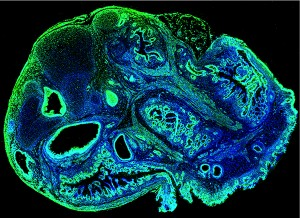
\includegraphics[width=0.8\columnwidth]{figures/cerebral_organoid/cerebral-organoid-for-Broad-web-300x218}
\caption{A cerebral organoid viewed under fluorescence microscopy \citep{nguyen_wang_nikolakopoulou_2015}.%
}
\end{center}
\end{figure}

\subsection{Brain development}

The mammalian brain is among the most complex organized structures in biology. The development of the animal nervous system, termed neural induction, is initiated by the formation of several primitive cell clusters early in development. This initial differentiation of neural progenitors begins with the formation of the neural plate on the ectoderm (outer layer) of the embryo, which folds inward to form the neural fold/groove, creating the neural tube and crest (Figure~\ref{fig:development}). 

\begin{figure}[h!]
\begin{center}
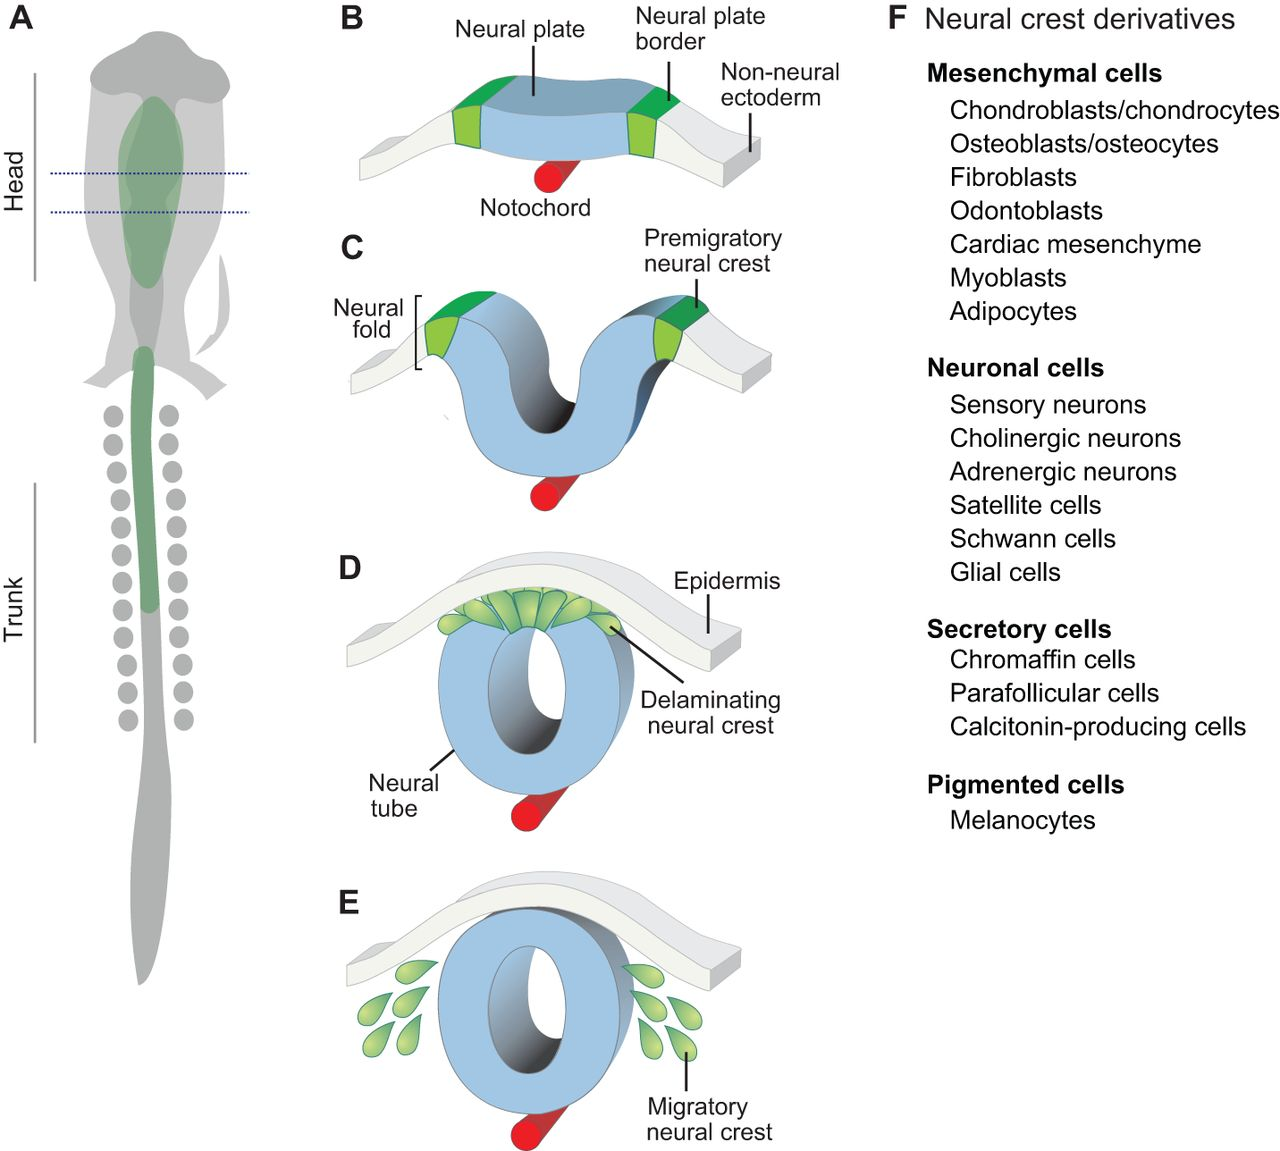
\includegraphics[width=0.8\columnwidth]{figures/brain_development}
\caption{Development of the neural tube \citep{neural_development}. \label{fig:development}%
}
\end{center}
\end{figure}

The neural tube is characterized by four regions which develop into distinct adult structures \citep{Bakken_2015}. The first of these, the prosencephalon, develops into the telencephalon and diencephalon, which further develop into the forebrain, hypothalamus, and eyes. The second region, the mesencephalon, develops into the midbrain. The third region, the rhombencephalon (named for its rhombus-like shape), is responsible for the lower regions of the brain such as the cerebellum, pons, and medulla oblongata, which originate from the metencephalon and myelencephalon. The last of these regions is the spinal chord.

\subsection{Gene expression regulation}\label{regulation}
Gene expression at the cellular level is regulated by a plethora of molecular means and is the foundation of an organism's development, growth, and survival. Although the vast majority of cells (except germ and certain immune cells) in an animal have identical DNA, their own structure and function is determined by these methods of regulation. This cellular regulation further determines the structure and function of the upper-level tissues, organs, and ultimately the organism itself. 

Gene expression consists of the processes of DNA transcription to RNA and RNA translation to the amino acid chain that becomes the protein. Transcription is influenced by transcription factors, which affect how well an RNA polymerase (the enzyme primarily responsible for transcription) is able to bind to and form a transcription complex on a gene. Specific examples of molecules affecting gene expression include the addition of acetyl or methyl groups to the DNA and proteins that by binding to the DNA, can either attract or block the binding of RNA polymerase. In eukaryotic cells such as those of mice and humans, the RNA transcript must be further processed prior to transcription. This post-transcriptional processing involves the addition of cap and tail sequences that protect the sequence from digestive enzymes and allow for translation to occur. The RNA transcript also contains exon and intron regions; only the exon regions are incorporated into the final sequence to be translated. Once the RNA transcript has left the nucleus of the cell (through a nuclear pore), a ribosome (a large cellular machine that facilitates translation of RNA to protein) binds to the RNA and initiates construction of the amino acid chain. Once the amino acid chain is complete, the ribosome splits in two, and the protein may be further modified. For instance, the chain may be folded within a chaperonin, which oversees the formation of the correct conformational design for some proteins, or the protein may be tagged with small molecules that identify its destination. These methods, and many others, allow for extremely precise regulation of complex genetic pathways that are the drivers of embryonic development.

The embryonic phase of development is known for highly dynamic expression of genes across time and space, or spatiotemporal regulation. Differential gene expression over space and time is the feature that allows an organism to develop specialized cells. Conditional regulation of only a  select few high-level "master genes" can determine the fate of a cell. 
\citep{bisceglia_2010}

\begin{figure}[h!]
\begin{center}
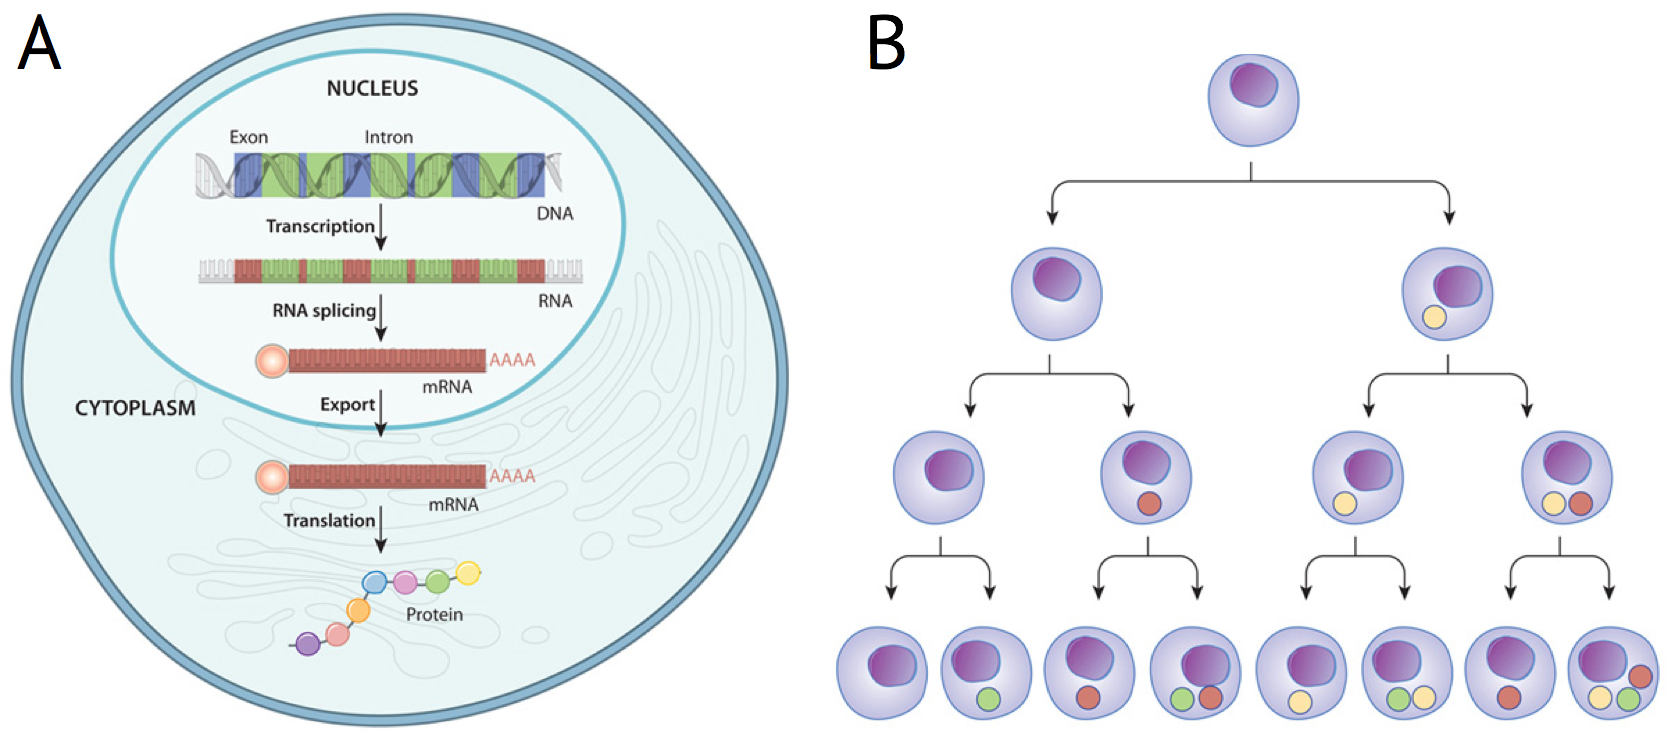
\includegraphics[width=0.8\columnwidth]{figures/Untitled/Untitled}
\caption{\textbf{A.} A general overview of the flow of information from DNA to RNA to protein. \textbf{B.} Demonstration of cell differentiation \citep{bisceglia_2010}.%
}
\end{center}
\end{figure}

\subsection{Gene expression measurement}
Numerous methods exist for the quantification and visualization of gene expression data. Two established methods include \textit{in situ} hybridization (ISH) and RNA sequencing (RNA-Seq). 

ISH is a technique that allows specific sequences of nucleic acids to be located in a section of cells or tissue. This localization is accomplished through the principle that complementary nucleic acid sequences form hydrogen bonds (hybridize) with each other. The complementary sequence, or the \textit{probe}, that detects the target sequence may be identified through fluorescent (fluorescent DNA components), radioactive (radioactive isotopes), or immunohistochemical (antibody-labeled) means. After the probe is allowed to hybridize to the target strand, RNases (RNA-digesting enzymes) hydrolyze any excess probes and the rest are washed off, leaving only bound probes behind. Following ISH, fluorescent microscopy may then be used to highlight regions of gene expression, which may then be scanned and analyzed using image analysis algorithms \citep{Angerer_1991}. Regions of high expression of the sequence of interest are shown as darker areas in an image (Figure~\ref{fig:ish}). 

In addition to ISH, RNA-Seq is also used in order to accurately measure gene expression. Because the primary function of RNA in the cell is as an intermediate in the transfer of information from DNA to protein, RNA expression levels can give an approximate indication of overall gene expression levels. In RNA-Seq, as the name suggests, next-generation nucleic acid sequencing is applied to a collection of RNA sampled from a tissue region. This RNA sample is first isolated from the source tissue through digestion using detergents and enzymes. Once the RNAs are isolated, a next-generation sequencing machine reads all the RNA to a digital storage device. These raw sequence data are then formatted to identify exons and introns, which may be later used to identify gene expression levels. These gene expression values provide an approximate indication of the degree of a gene's expression within a cell \citep{Wang_2009}.

\begin{figure}[h!]
\begin{center}
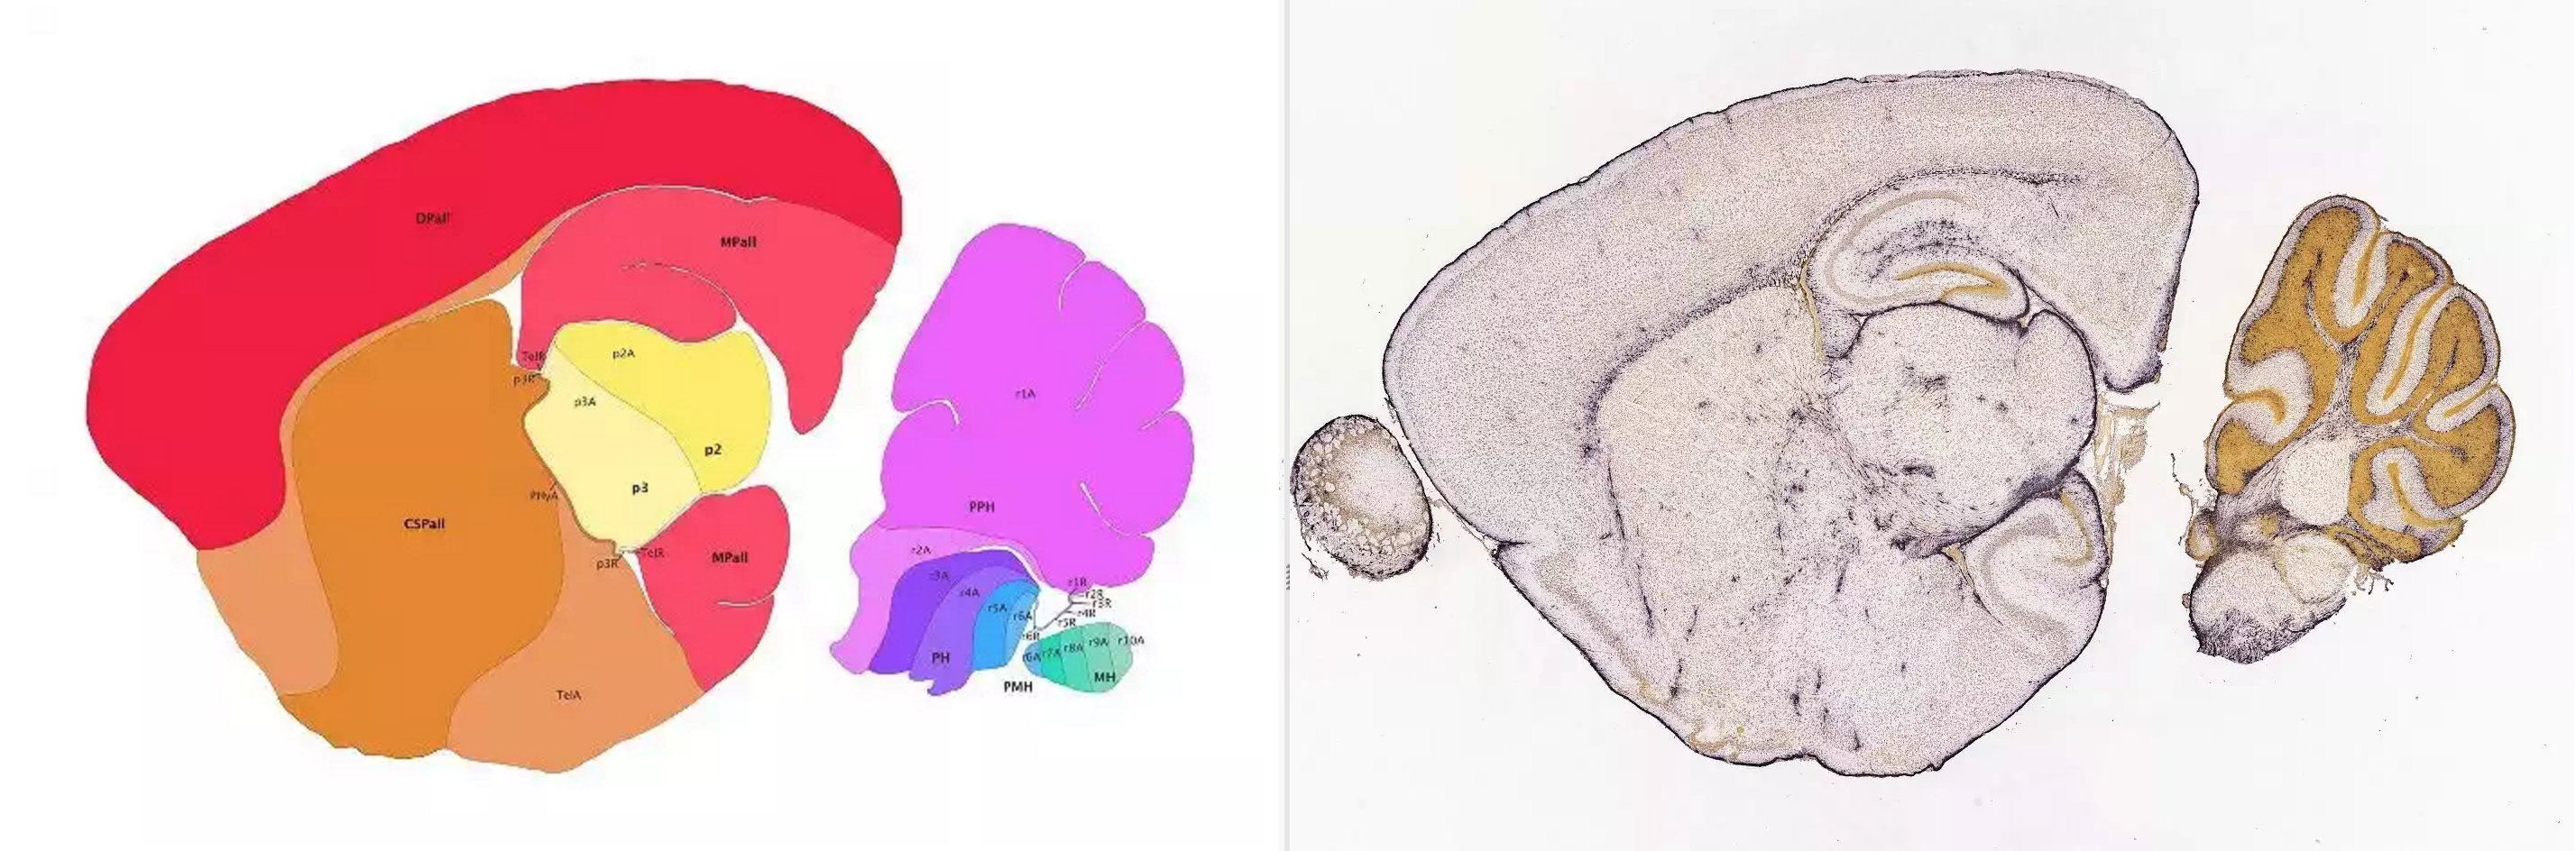
\includegraphics[width=0.8\columnwidth]{figures/ISH/ISH}
\caption{An ISH stain for glial fibrillary acidic protein (GFAP) RNA in the P14 mouse brain. At left is a diagram of the regions shown in the staining for reference (Allen Brain Atlas).\label{fig:ish}
}
\end{center}
\end{figure}

\subsection{Gene expression analysis}\label{gene_analysis}

Gene expression values offer valuable insights into the dynamics of regulatory networks and cellular processes. Analyses may be performed at any level of regulation described in Section~\ref{regulation}. Among one of the most widely used expression analysis techniques are those which cluster genes by similarity of expression. The clusters obtained using these methods can be used to generate dendrograms (Figure~\ref{fig:leukemia}) that provide a hierarchical ordering of the genes. Genes within a cluster are assumed to share a common underlying biological mechanism of action that is responsible for similar expression patterns.

The accuracy of a clustering depends heavily on the hyperparameter $K$, which denotes the number of clusters. In hierarchical clustering, a determining an optimal value of $K$ is equivalent to determining the level at which the produced dendrogram is cut. An excessively low $K$ may lead to large clusters which provide an overly general fit to the genes and fails to provide any meaningful insight. An excessively high $K$, on the other hand, may create more clusters than is necessary and creates categories where there are none. The validity of the clustering may be assessed by removing one of the predictor variables (for instance, a specific timepoint or region of expression), and examining whether or not the resultant clustering is significantly altered \citep{how_expression_works}. A significantly altered clustering would suggest that one variable affects the clustering to an abnormal degree, which may imply that the clustering method is chaotic.

\begin{figure}[h!]
\begin{center}
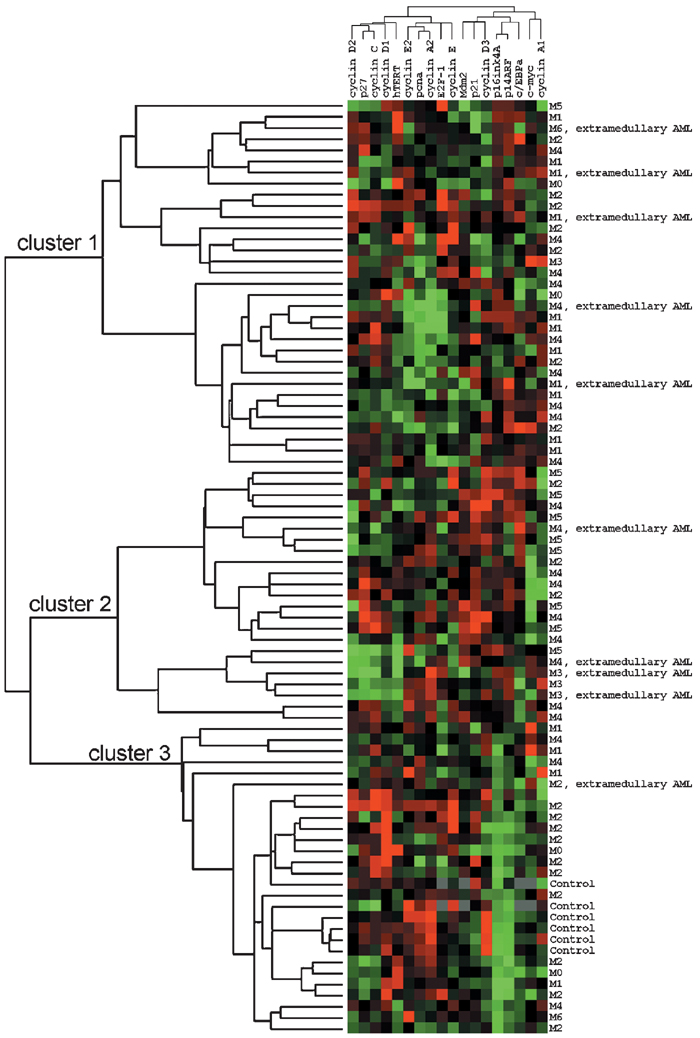
\includegraphics[scale=0.25]{figures/leukemia_clustering}
\caption{An example of a clustering algorithm applied to expression values of genes related to acute myeloid leukemia. Dendrograms were created for regions (top) and sample (left) \citep{leukemia_clustering}.\label{fig:leukemia}
}
\end{center}
\end{figure}

\subsection{The Allen Brain Atlas}
Founded in 2003 by Microsoft co-founder Paul Allen, the Allen Institute for Brain Science is a nonprofit research organization dedicated to the public pursuit of brain research. Among the many free datasets provided by the Institute are the Allen Developing Mouse Brain Atlas (located at \href{http://www.developingmouse.brain-map.org/}{www.developingmouse.brain-map.org/}) and the Allen Atlas of the Developing Human Brain (located at \href{http://www.brainspan.org/}{www.brainspan.org/}).

The Developing Mouse Brain Atlas features in situ hybridization (ISH) data for over 2,100 genes across multiple stages of embryonic and postnatal mouse brain development. The raw images of the ISH scans total 434,946 images. These images were assembled into 3-dimensional grids of expression values.  In addition, an application programming interface (API) in the form of a bioinformatics pipeline allows researchers to access all data produced by the Developing Mouse Brain studies. The Developing Mouse API further allows researchers to obtain quantized expression values per region, which are calculated based off of analysis of the ISH scan images. These expression values may be found for several different developmental time points, at several discrete brain regions, for each of the 2,100+ genes \citep{Thompson_2014}.

Similar to the Developing Mouse Brain Atlas, the Developing Human Brain Atlas also features a diverse array of ISH expression values for several thousand genes. These expression values are available for download as raw comma-separated-values (CSV) files from the Developing Human Brain Atlas Website, although an API is still available. In addition to ISH images, extremely detailed, cellular-level, magnetic resonance imaging (MRI) and microarray data are also included \citep{24695229}. The expression levels for these images may be summarized using image analysis techniques provided by the Brain Atlas API which yield region-time expression matrices (Figure~\ref{fig:matrix}).

\begin{figure}[h!]
\begin{center}
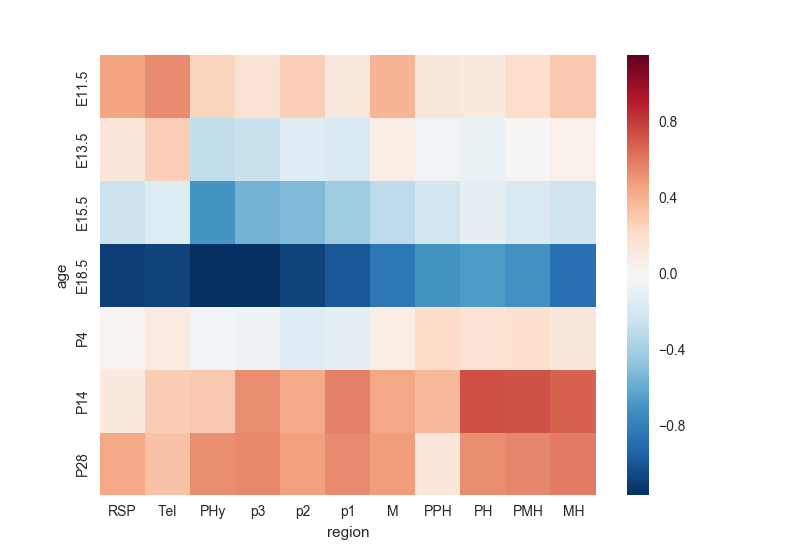
\includegraphics[width=0.8\columnwidth]{figures/Abl1/Abl1}
\caption{A heatmap of expression values for the Abelson murine leukemia viral oncogene homolog 1 (ABL1) gene in the developing mouse brain. Expression values were obtained from ISH stains and computed for each region using specialized 3-D voxel counts provided by the Allen Brain Atlas API. The y-axis is the development stage and the x-axis is the brain region (abbreviated). The expression values were transformed to a logarithmic scale to account for skew. \label{fig:matrix}%
}
\end{center}
\end{figure}

\subsection{Neural networks}
Neural networks are a subfield of machine learning, which is often cited as the ``field of study that gives computers the ability to learn without being
explicitly programmed," a definition given by Arthur Samuel in 1959. Although invented around the mid 19-th century \citep{Zilouchian2001FundamentalsON}, neural networks today are one of the most flexible and powerful machine learning algorithms. In several areas of research, neural networks offer state-of-the-art performance over traditional, hand-coded methods, such as in image pattern recognition, genomic analysis, and protein folding prediction. The basic neural network node, or \textit{neuron}, is similar to its biological counterpart in that it receives a number of inputs and outputs an output (Figure~\ref{fig:neuron}). However, the two differ in both structure and function. For instance, the biological neuron asynchronously receives a combination of excitatory and inhibitory impulses and sends a constant output signal. An artificial neuron instead is a mathematical construct that receives inputs synchronously and usually has a variable output value. In addition, whereas biological neural networks tend to be complicated in their topologies (many are not yet understood), artificial neural networks almost always have a tree-based structure of connectivity. The two further differ in their application: whereas brains are capable of extrapolation and learning of novel tasks, artificial neural networks are specialized and cannot readily adapt to new tasks given learned information.

\begin{figure}[H]
\begin{center}
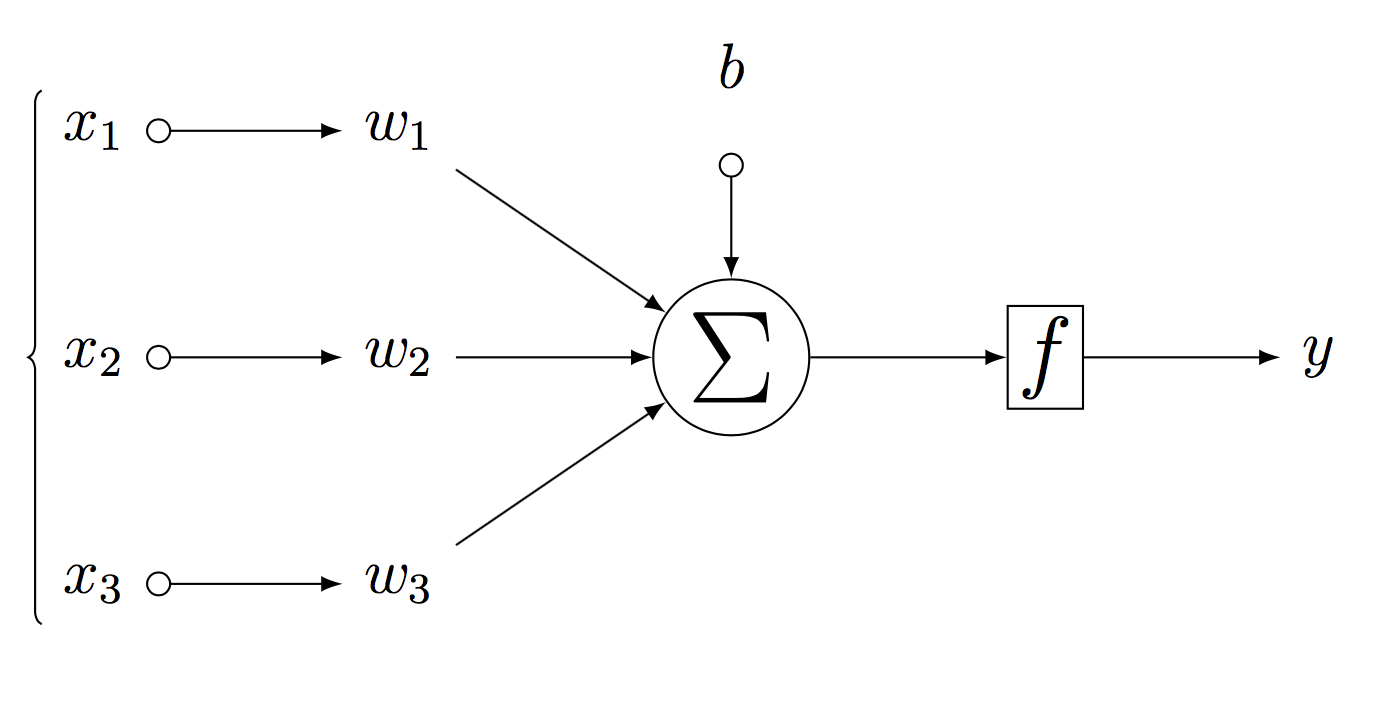
\includegraphics[width=0.8\columnwidth]{figures/neuron}
\caption{A diagram of a basic neuron with input values $x_{1}$,$x_{2}$, and $x_{3}$ with respective weights $w_{1}$,$w_{2}$, and $w_{3}$ and a bias $b$. The neuron computes the sum of these inputs and outputs a value $y$ determined by activation function $f$. \label{fig:neuron}}
\end{center}
\end{figure}

Neural networks learn by minimizing an objective function which determines the degree of error present in the predictions of a network. This objective function is used to drive gradual minimization of the error rate, which is accomplished by adjusting the specific weights and biases in a network. When a network is first initialized, the weights present are usually set to zero or randomly determined using a probability distribution function. As the network is fed data, the outputs are compared to target values and a loss value is computed. This loss value is then used to adjust the weights of the network to better fit the inputs to the output using a method called backpropagation. The effect of each neuron on the loss function is computed using the chain rule, which allows for the computation of the gradient of cost function. The weights are then updated using a method of gradient descent in order to minimize the loss value. This iterative updating allows the network to eventually learn a complex function given enough training data and time \citep{Zilouchian2001FundamentalsON}. 

There exist a multitude of activation functions which determine the output of an artificial neuron (Figure~\ref{fig:activations}). Many of these functions are designed such that the loss gradients have smooth derivatives that can be handled by backpropagation. For instance, a step function would not be able to be backpropagated. The activation functions will also partly determine the computational workload; a ReLU activation gradient, having one of two constant derivatives, requires less processing power than a sigmoid activation gradient.

\begin{figure}[H]
\begin{center}
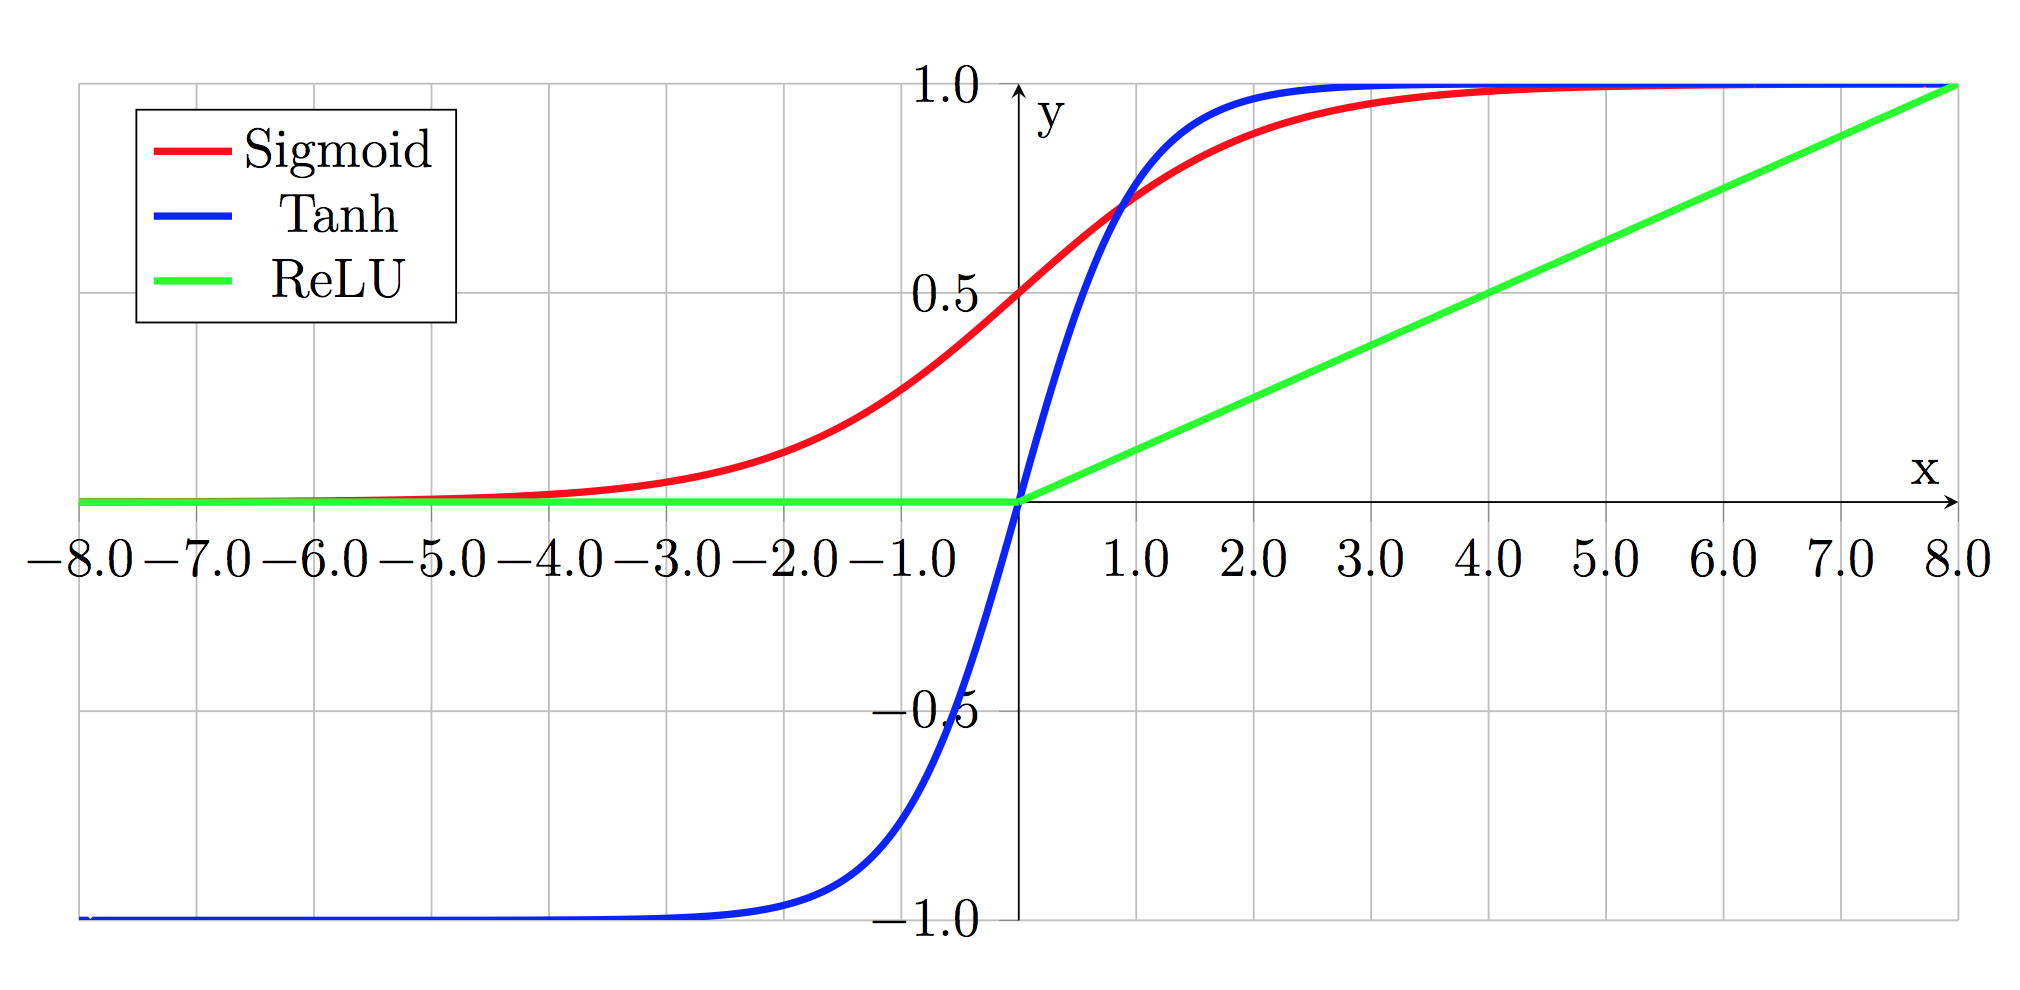
\includegraphics[width=0.8\columnwidth]{figures/activations}
\caption{Graphs of common neuron activation functions.\label{fig:activations}}
\end{center}
\end{figure}

\begin{table}[H]
\begin{center}
\caption{Equations of the activation functions shown in Figure~\ref{fig:activations}.}
\begin{tabular}{ l | l | l | l }
 Linear & Sigmoid & Tanh & ReLU\\ 
 $a(x) = x$ & $a(x) = \frac{1}{1+e^{-x}}$ & $a(x) = \frac{e^{x}-e^{-x}}{e^{x}+e^{-x}}$ & $a(x) = 0\ \textrm{if}\ x \leq 0, x\ \textrm{if}\ x > 0$\\   
\end{tabular}
\label{table:1}
\end{center}
\end{table}

Neural networks are able to approximate complex functions such as classifiers through abstraction by multiple layers. In general, larger neural networks tend to yield more accurate predictions and lower losses. However, large networks are very computationally expensive to train and may also overfit the data when there are not enough training examples \citep{Zilouchian2001FundamentalsON}.

\begin{figure}[H]
\begin{center}
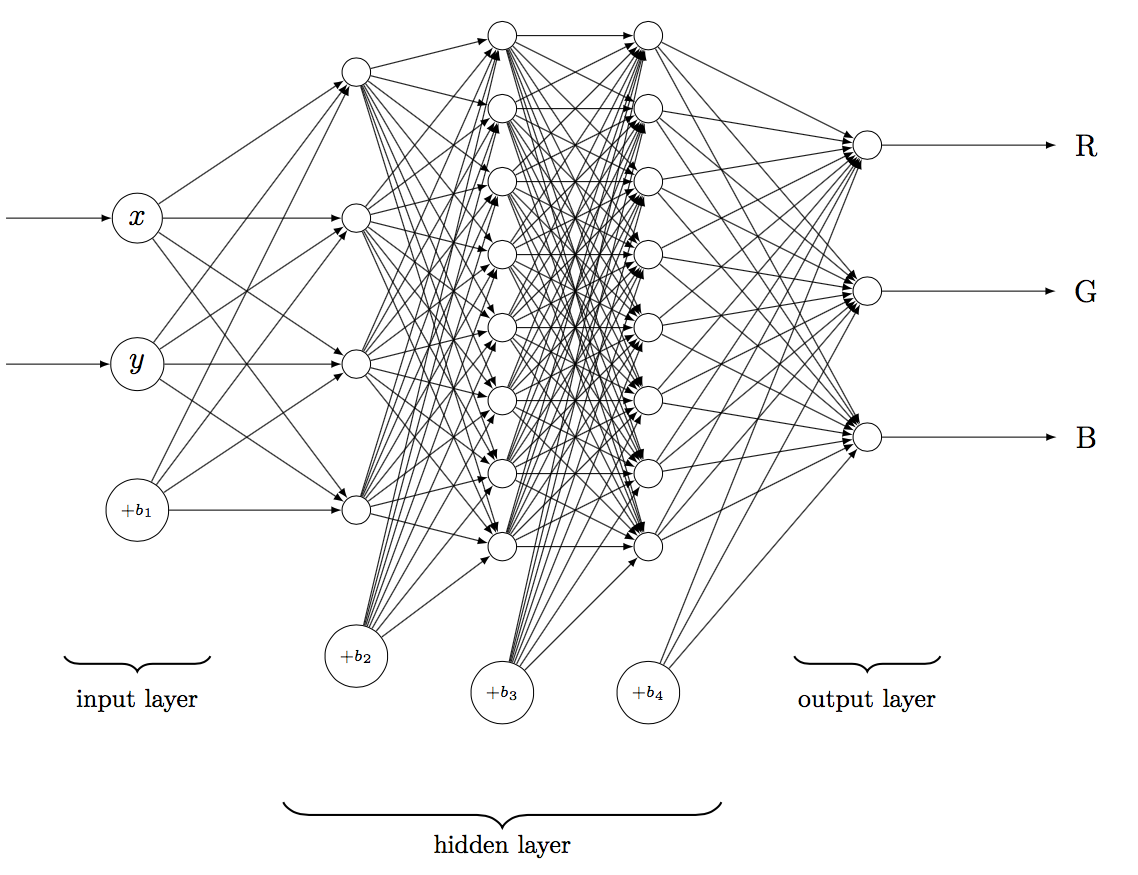
\includegraphics[width=0.8\columnwidth]{figures/doodle}
\caption{An example neural network that learns to generate an image given x and y pixel position inputs. The inputs are the x and y coordinates of the pixel, and the outputs are the three red-green-blue (RGB) values that define the color of a pixel.
\label{fig:doodle}
}
\end{center}
\end{figure}

In image analysis, a specific type of neural network termed the convolutional neural network is often used. Convolutional neural networks are loosely based on the structure of the animal visual cortex, which contains overlapping receptive fields. Similarly, in the convolutional neural network architecture, the inputs to a neuron are shared, convolving the input image. In a convolutional layer, the inputs are processed using filters, which are the two-dimensional representations of the weights used by each unit, or kernel, of the layer. These filters are gradually adjusted during training to recognize specific features in the input. The results of the convolution are then processed using a pooling method (Figure~\ref{fig:convolutional_mnist}) that produces a more abstract representation. In deep learning, convolutional and pooling layers are often coupled in a sequence such that higher level features may be learned from the data. For example, while the first layer of convolution may be trained to recognize edges, later layers may recognize shapes and eventually discrete objects. The primary advantage of convolutional neural networks lie in the fact that they are locally scale-invariant: convolution allows a feature of the image to be recognized regardless of position \citep{Krizhevsky2012ImageNetCW}.

\begin{figure}[H]
\begin{center}
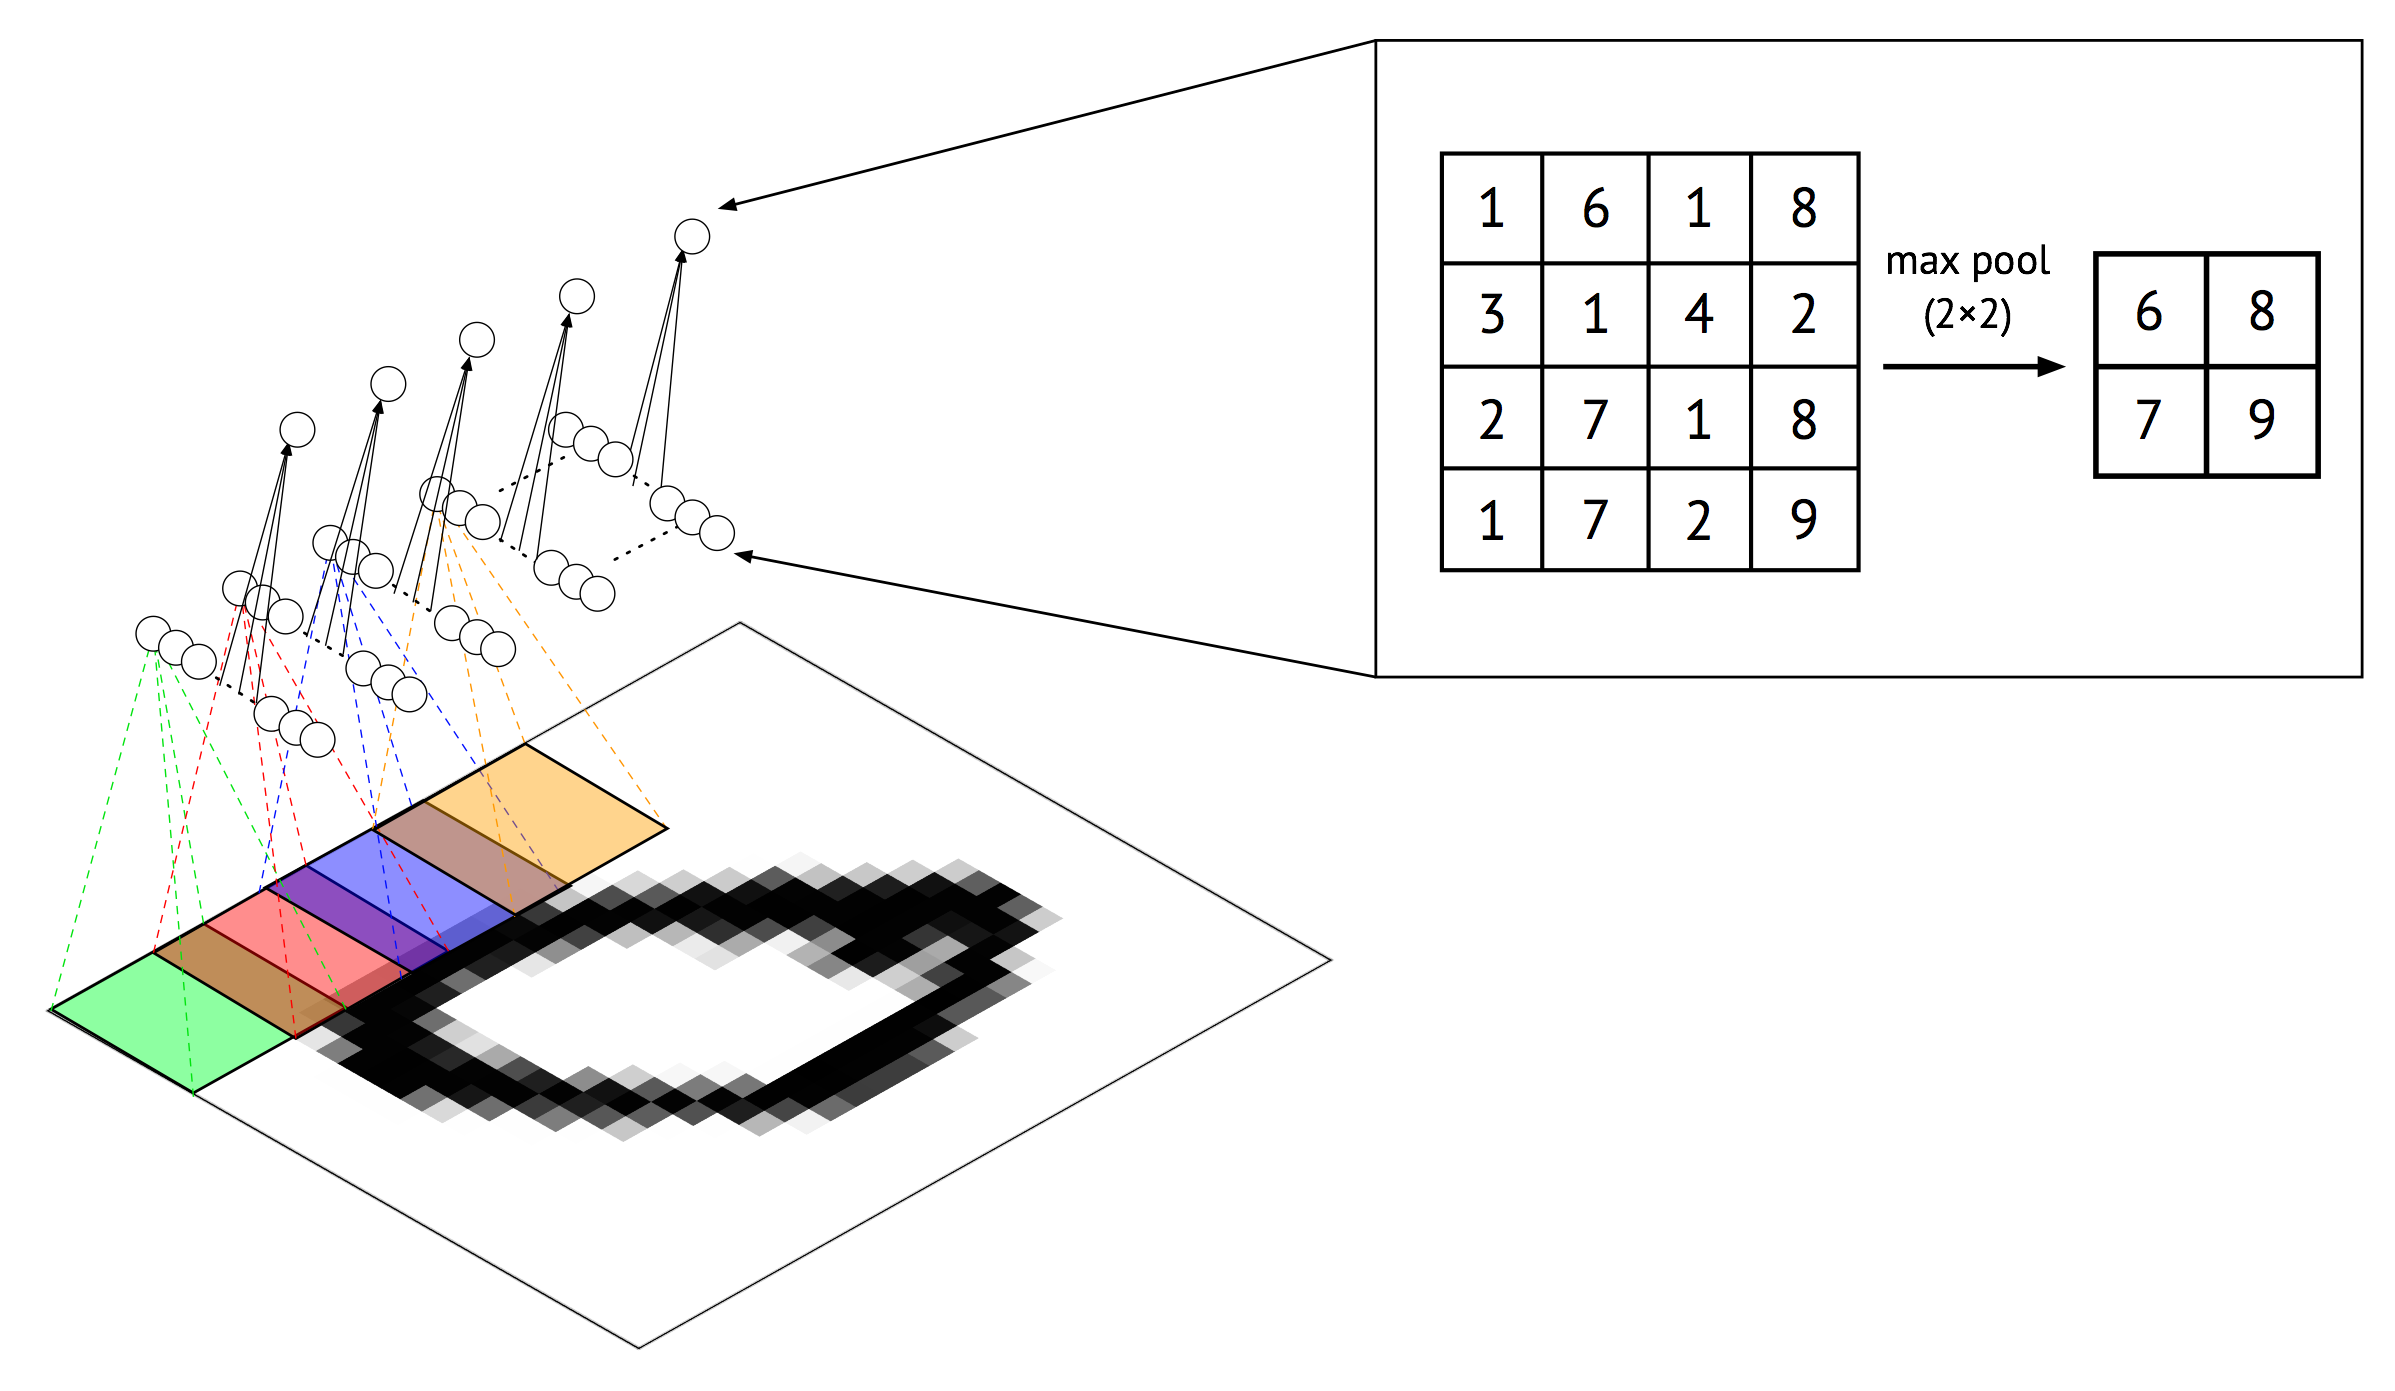
\includegraphics[width=0.8\columnwidth]{figures/convnet}
\caption{An example of a simple convolutional network designed for digit classification of the MNIST dataset. \label{fig:convolutional_mnist}}%
\end{center}
\end{figure}

Following convolution and pooling layers, a dense layer of neurons is implemented to classify the features obtained (Figure~\ref{fig:mnist_full}). Variations of these networks are currently considered state-of-the-art in nearly all image classification tasks \citep{Koushik2016UnderstandingCN}.

\begin{figure}[H]
\begin{center}
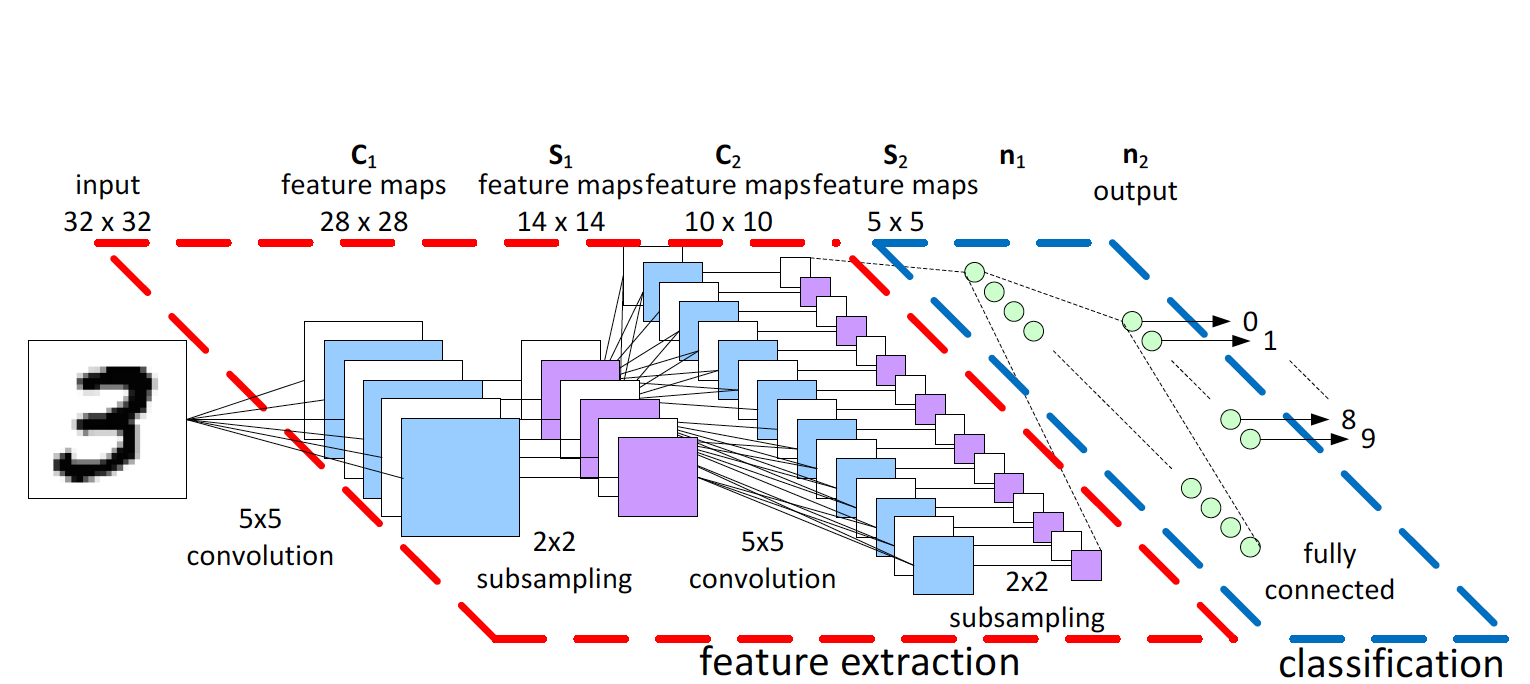
\includegraphics[width=0.8\columnwidth]{figures/CNN/CNN}
\caption{An example of a multi-layer CNN for classifying handwritten digits from the MNIST dataset. The feature extraction section repeatedly convolves the input image to higher level features, which are fed as inputs to the classification stage. In this case, the classification stage is composed of two fully connected layers, with the final layer outputting the predicted digit classification \citep{peemen_mesman_corporaal_2011}. \label{fig:mnist_full}%
}
\end{center}
\end{figure}

\subsection{Unsupervised learning}

Machine learning can be divided into the two subfields of unsupervised and supervised learning. The primary difference between the two is in the training of the model: supervised learning trains the model using a predefined set of classifications, or \textit{labels}, unsupervised learning trains the model without such guidance. Figure~\ref{fig:super} gives a basic illustration of the difference between the two:
in the left diagram, the datapoints are labeled as being red hexagons or blue triangles. With these labels, one could train supervised programs such as classifiers that predict the label of a data point given its x-y position. On the figure on the right, however, none of the datapoints are labeled (all of them are red hexagons). For these data, one could apply an unsupervised method such as a clustering analysis program to group datapoints by how similar they are to each other. This allows researchers to make inferences regarding patterns and structures in the data.

\begin{figure}[H]
\begin{center}
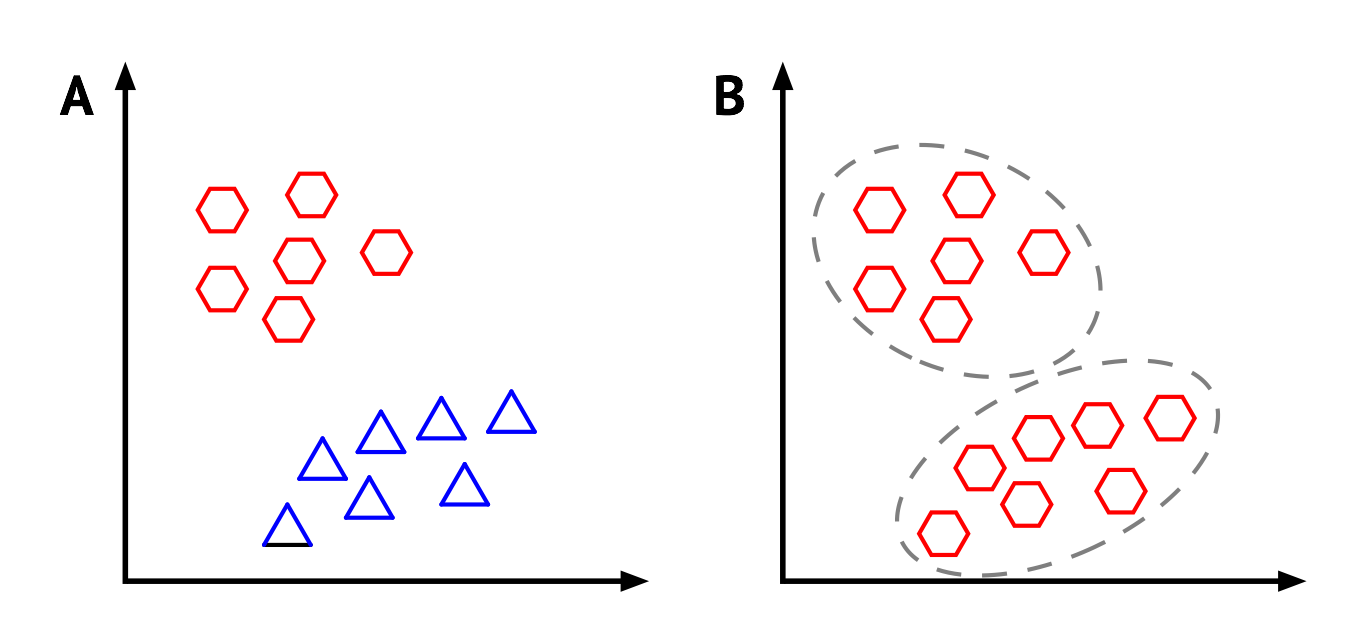
\includegraphics[width=0.8\columnwidth]{figures/learningtypes}
\caption{An illustration of the primary difference between supervised (\textbf{A}) and unsupervised (\textbf{B}) learning.\label{fig:super}
}
\end{center}
\end{figure}

Clustering is an essential method of unsupervised learning. Clustering analysis is often performed following dimensionality reduction methods that allow the data to be reduced to a simple two or three-dimensional representation while maintaining the original variance and structure in the data. Algorithms such as K-means, DBSCAN, and complete linkage clustering may then be employed to calculate clusters. In image classification tasks, classification and dimensionality reduction allow the learned results of a neural network to be visualized (Figure~\ref{fig:clusters}). Furthermore, a convolutional neural network may be directly coupled with a clustering algorithm as a loss function in order to gradually produce high quality clusters as the network is trained \citep{yangCVPR2016joint}.

\begin{figure}[H]
\begin{center}
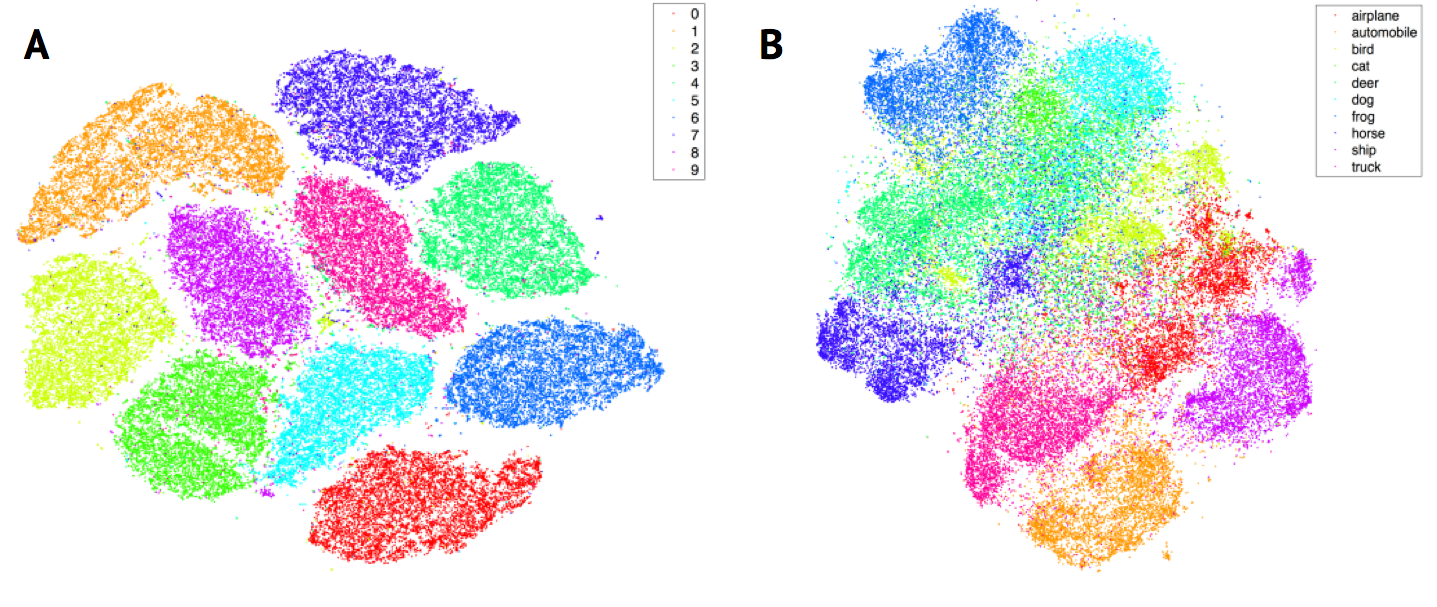
\includegraphics[width=0.8\columnwidth]{figures/tsne}
\caption{The results of a t-Distributed Stochastic Neighbor Embedding (t-SNE) dimensionality reduction on a clustering of the MNIST (\textbf{A}) and CIFAR-10 (\textbf{B}) datasets \citep{laurensvandermaaten2014}. \label{fig:clusters}%
}
\end{center}
\end{figure}

\section{Research plan}


\subsection{Researchable question}
Are there significant differences between patterns of gene expression in developing mouse and human central nervous systems?

\subsection{Hypothesis}

It was hypothesized that significant differences exist between the gene expression profiles of developing mouse and human central nervous systems.

\subsection{Procedure}
This project was entirely performed on a computer. Gene expression profiles for developing mouse and human brains were first downloaded from the Allen Brain Atlas. Next, the data were formatted and transformed into sets of region versus time expression matrices into two datasets, a developing human dataset and a developing mouse dataset. 

For each dataset, a convolutional neural network algorithm was applied in order to automatically classify genes into discrete clusters based on patterns of expression. The relative positions of genes in the human and mouse clusterings were examined. Different clusterings would suggest that the transcriptomic landscapes are different. The gene expression clusterings may be applied to highlight discrete drug-gene interactions in human versus mouse brains. Potential differing expressions may account for anatomical differences in mouse and human brains. As an extension, the similarity of expression patterns in cerebral organoids will also be considered. The insights from this project may also be applied to single-cell cancer sequencing, where clustering analysis may be used for the characterization and identification of stages of cancer cell development.

\section{Methodology}

\subsection{Overall workflow}

The overall process consisted of the retrieval, formatting, dimensionality reduction, and comparison of neural gene expression data. Gene expression profiles for both mouse and human donor brains were obtained from the Allen Brain Atlas website through either direct download (human) or a script (mouse). Expression values were log2-transformed and normalized to a (-1,1) range. A convolutional autoencoder (CAE) was constructed and embedded each 77 (mouse) or 150 (human) -dimensional expression matrix onto a four-dimensional manifold. t-distributed stochastic neighbor embedding (t-SNE) was then applied to further reduce the dimension count to two. This dimensionality reduction method was compared to traditional methods using only principal component analysis (PCA) and t-SNE in published literature. Density-based spatial clustering of applications with noise (DBSCAN) was then used to identify clusters in the two-dimensional space in each mouse and human dataset. These clusterings were compared using the adjusted rand index (ARI) and mutual information score. In addition, this study also compared the CAE-based method with the results obtained by existing correlation-based hierarchical clustering of the raw expression values.

\begin{figure}[H]
\begin{center}
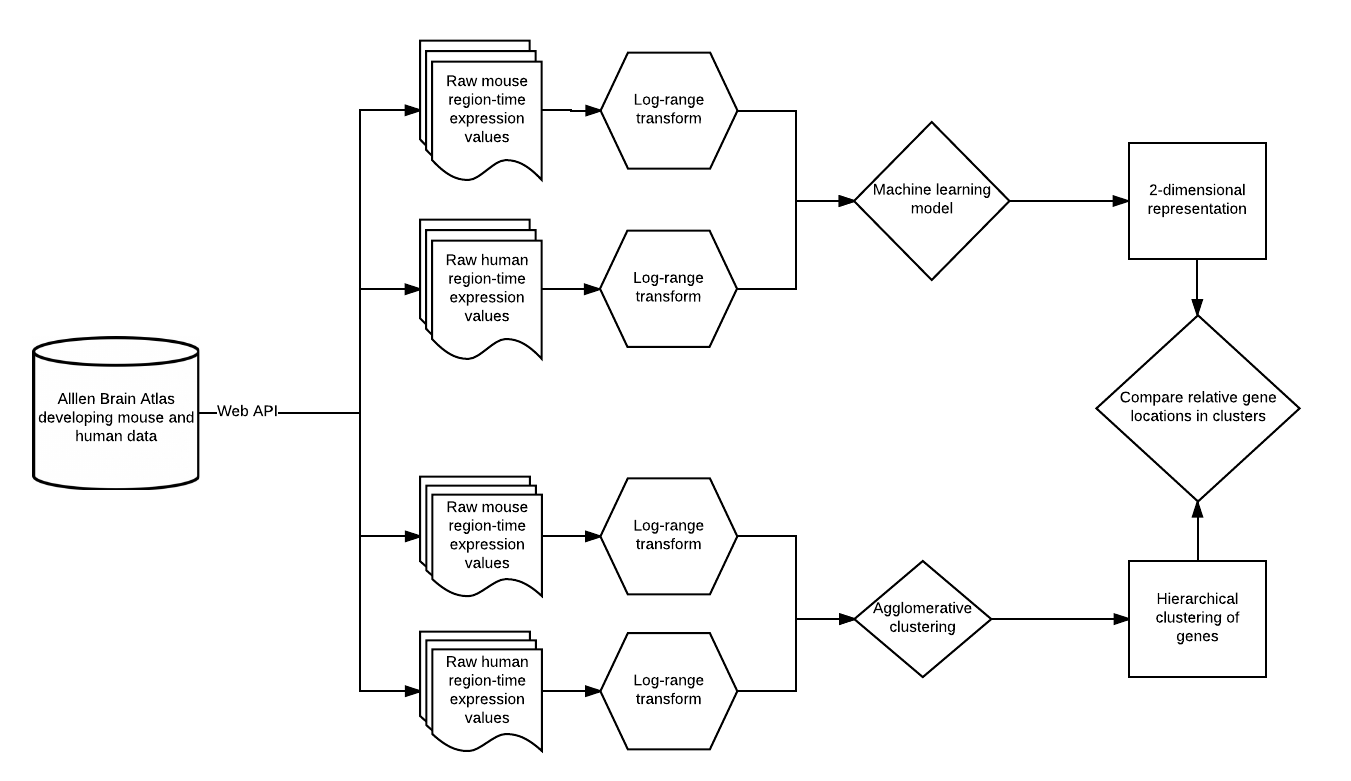
\includegraphics[width=0.9\columnwidth]{figures/workflow}
\caption{The overall process involved in this project. \label{fig:workflow}%
}
\end{center}
\end{figure}

\subsection{Software}

A number of open-source software packages and modules were used in this project. A script written in Ruby 2.0.0 was used to extract the mouse expression matrices from the Allen Brain Atlas API. Python 3.5.1 was used to perform all further analysis. Raw expression values for both the mouse and human datasets were manipulated using the Pandas package. Numpy was used for manipulation of the unlabeled expression matrices. The convolutional autoencoder was constructed with the aid of the Keras and Tensorflow \citep{tensorflow2015-whitepaper} frameworks. The SciPy package was used for hierarchical clustering analysis, dendrogram construction, Pearson and Spearman correlation analyses, and distance matrix construction. The scikit-learn package was used for t-SNE, DBSCAN, PCA, and computation of the adjusted rand indices and mutual information scores. Graphs and other visualizations were constructed using the Matplotlib, Seaborn, and Plotly libraries. Gephi and D3.js were used for visualization of the correlation graphs.

\subsection{Data retrieval}

Mouse raw expression values were obtained using a Ruby script provided by the Allen Brain Institute under the Apache 2.0 License. This script utilized the RESTful Model Access (RMA) service to download approximately 2,100 expression profiles. Each expression profile was produced using image analysis algorithms to summarize ISH stains of tissue sections. A full expression profile of a gene in the mouse dataset contained 77 values describing expression over 11 regions and 7 timepoints. 

Human expression values for approximately 52,000 genes were obtained from downloading the Developmental Transcriptome Dataset located on \url{http://www.brainspan.org/static/download.html}. These expression values were compiled using quantization of RNA-seq results. The raw human data contained over 500 region-timepoint combinations. Of these, 10 common regions and 15 common timepoints were identified using a search algorithm to maximize the number of shared regions and timepoints.

\subsection{Data pre-processing}

Mouse and human datasets were first compared and filtered to 1,912 orthologs (shared genes). Raw expression values were further transformed by taking the base 2 logarithm, resulting in a more symmetrical distribution. This transformation was performed because the raw distribution was found to have high right skew (Figure~\ref{fig:log2}). The data were also normalized to the interval [-1,1] using a proportional transformation. This was done due to the nature of the neural network architecture, which uses a hyperbolic tangent function on the output layer, resulting in a possible output interval of (-1,1).

\begin{figure}[H]
\begin{center}
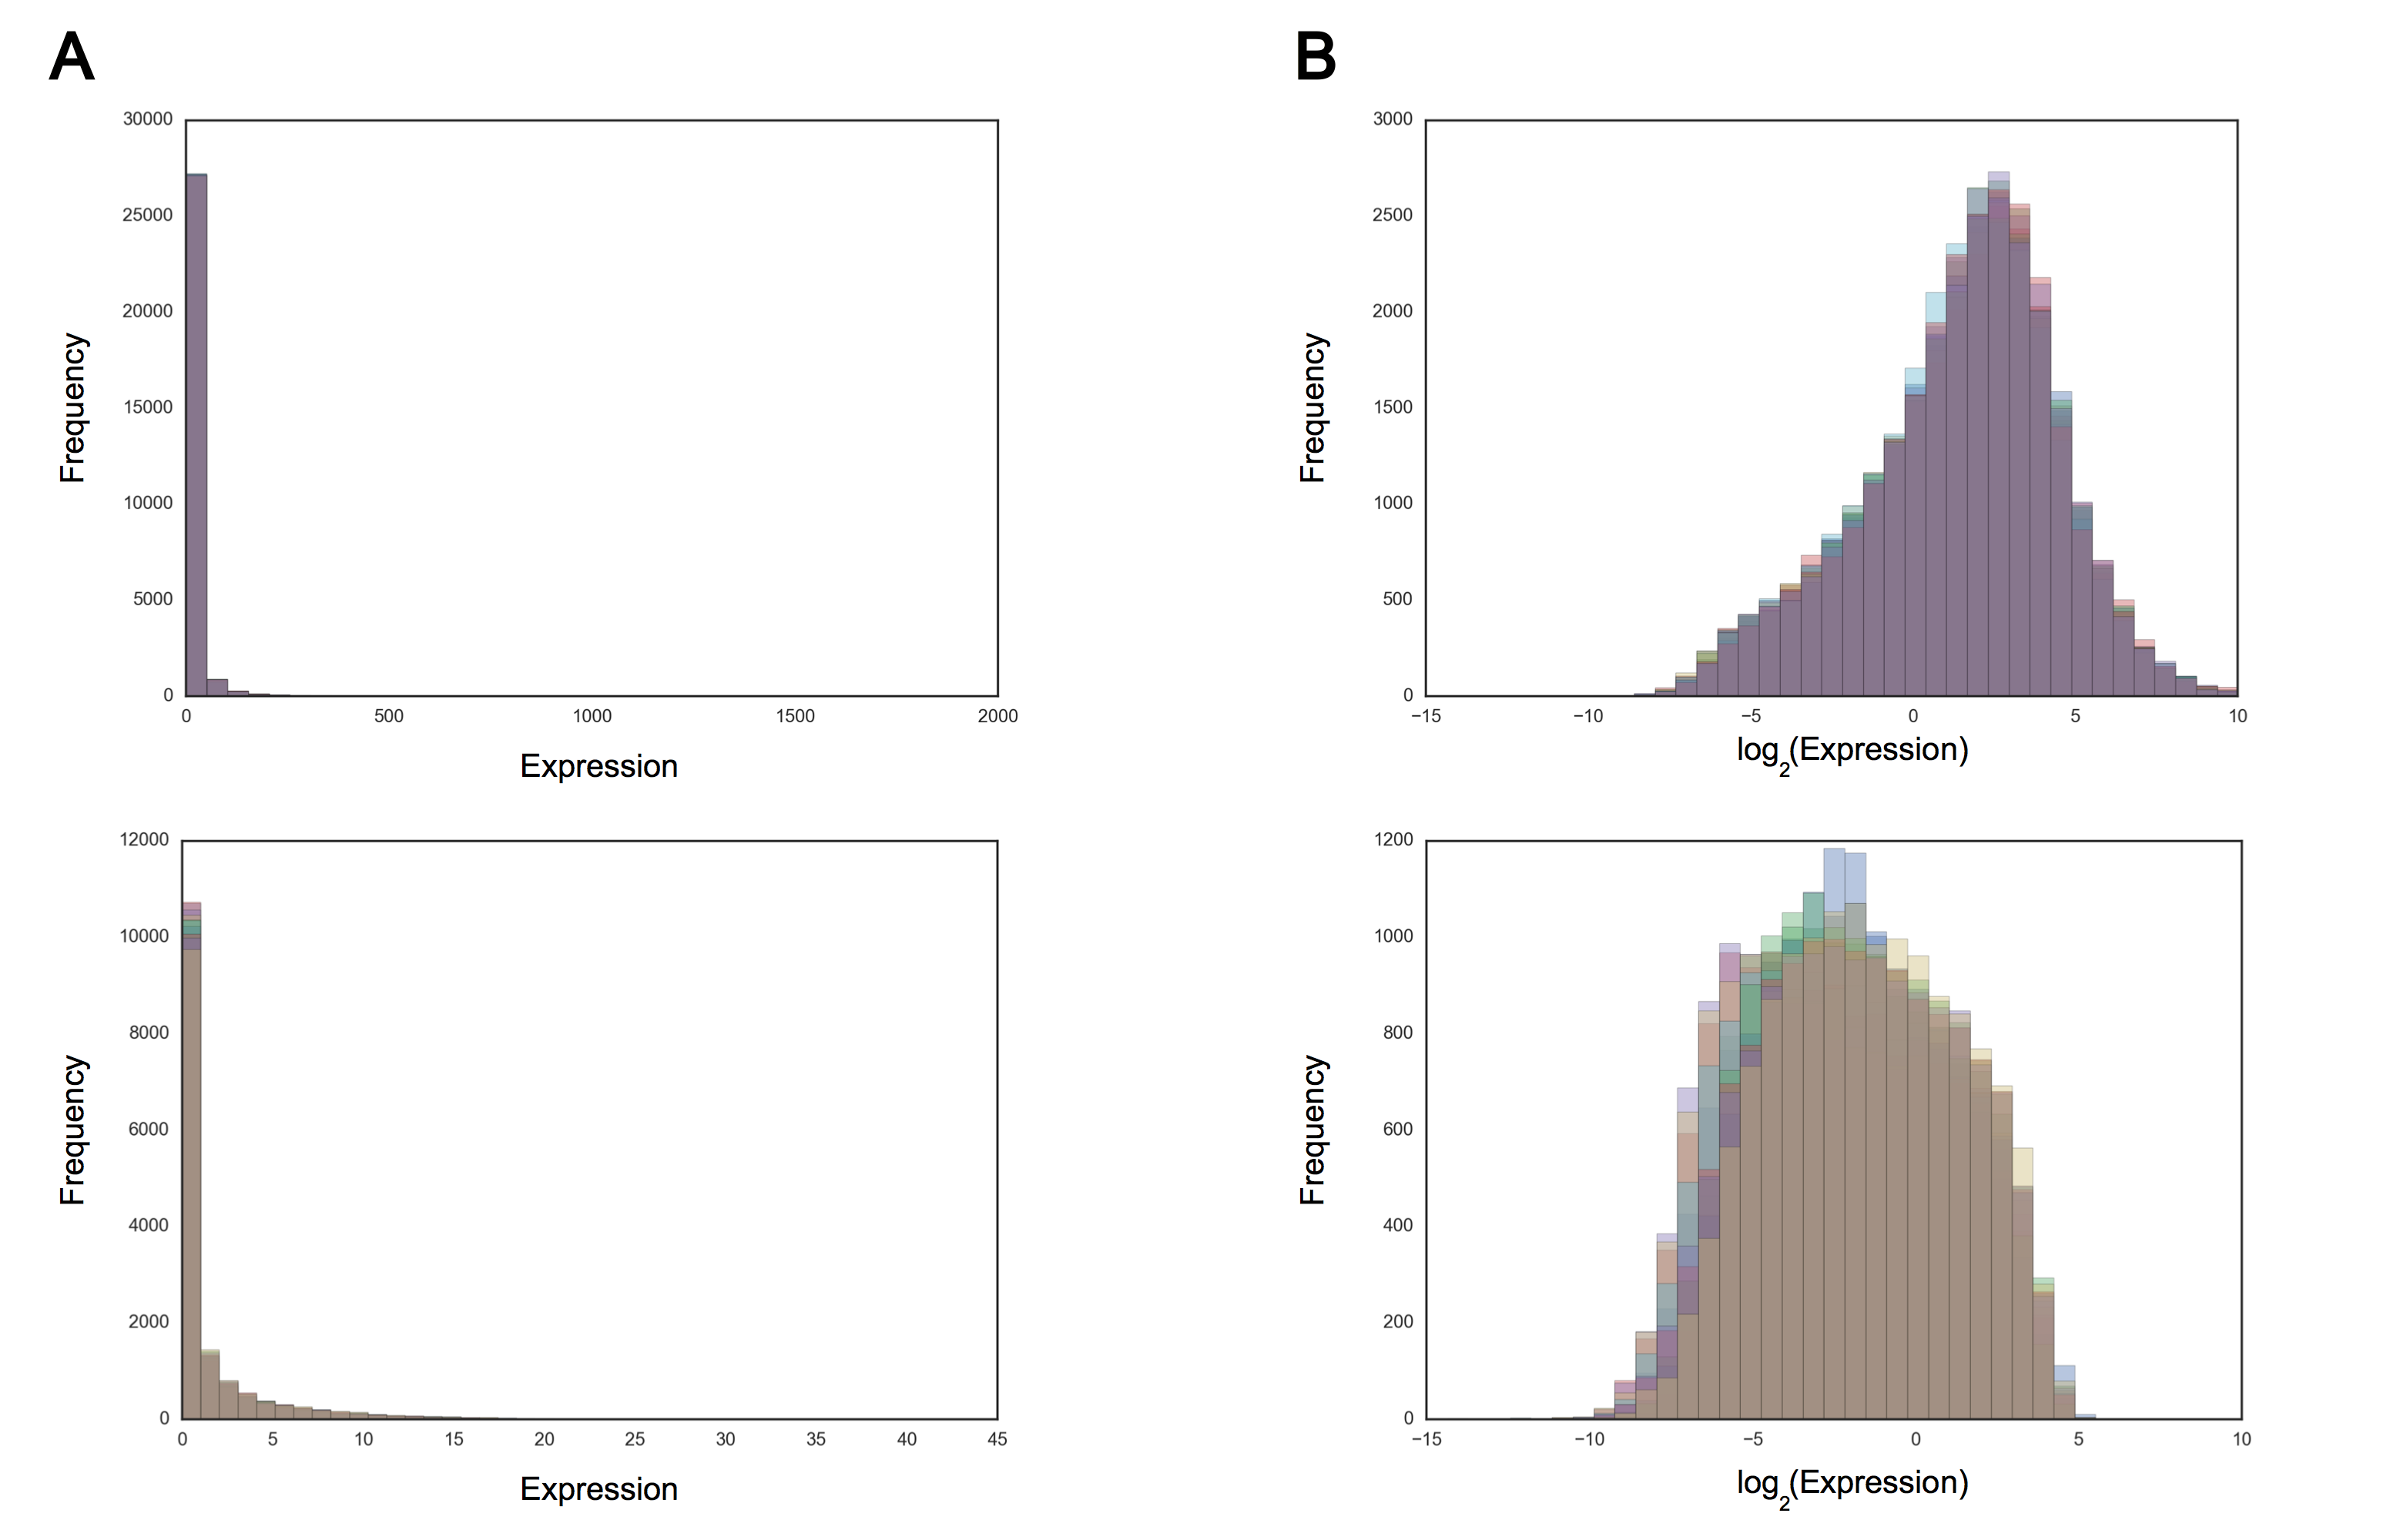
\includegraphics[width=0.9\columnwidth]{figures/log2}
\caption{Comparison between (\textbf{A}) raw expression values and (\textbf{B}) log2-transformed expression values for each region between the human (top) and mouse (bottom) datasets. \label{fig:log2}%
}
\end{center}
\end{figure}

\subsection{Machine learning model}


A machine learning model was then constructed to reduce the dimensionality of each dataset to two dimensions. This program consisted of two main methods, a convolutional autoencoder (CAE) and a t-distributed stochastic neighbor embedding (t-SNE) that functioned sequentially. 

The CAE was composed mainly of convolutional encoding, dense hidden, and convolutional decoding layers (Figure~\ref{fig:CAE}). Because 2 by 2 max pooling layers require even dimensions to function correctly, the mouse expression profiles were first mapped using a dense network to a single 8 by 8 representation from the original 7 by 11 layer. Similarly, human expression profiles were mapped to a 16 by 8 representation from the original 15 by 10. The convolutional encoding layers then reduced each expression profile to four 2 by 2 (mouse) or 4 by 2 (human) filtered representations, which were transformed into a 16- or 32-dimensional representation as the input to the dense hidden network. This representation was then mapped to a four-dimensional representation in the center of the neural network. The convolutional decoding layers functioned in the opposite manner of the convolutional encoding layers. For example, max pooling layers in the encoder were replaced with upsampling (interpolation) layers in the decoder. 

The CAE was then trained on each dataset individually with the cost function being the root mean squared error (RMSE) between the two groups given by

$$\sqrt{\frac{\sum_{i}^n (\hat{y}_i-y_i)^2}{n}}$$

\noindent 
where $n$ is the number of individuals, $y_{i}$ is the dependent variable in a regression, and $\hat{y}_{i}$ is the prediction output of the model.


\begin{figure}[H]
\begin{center}
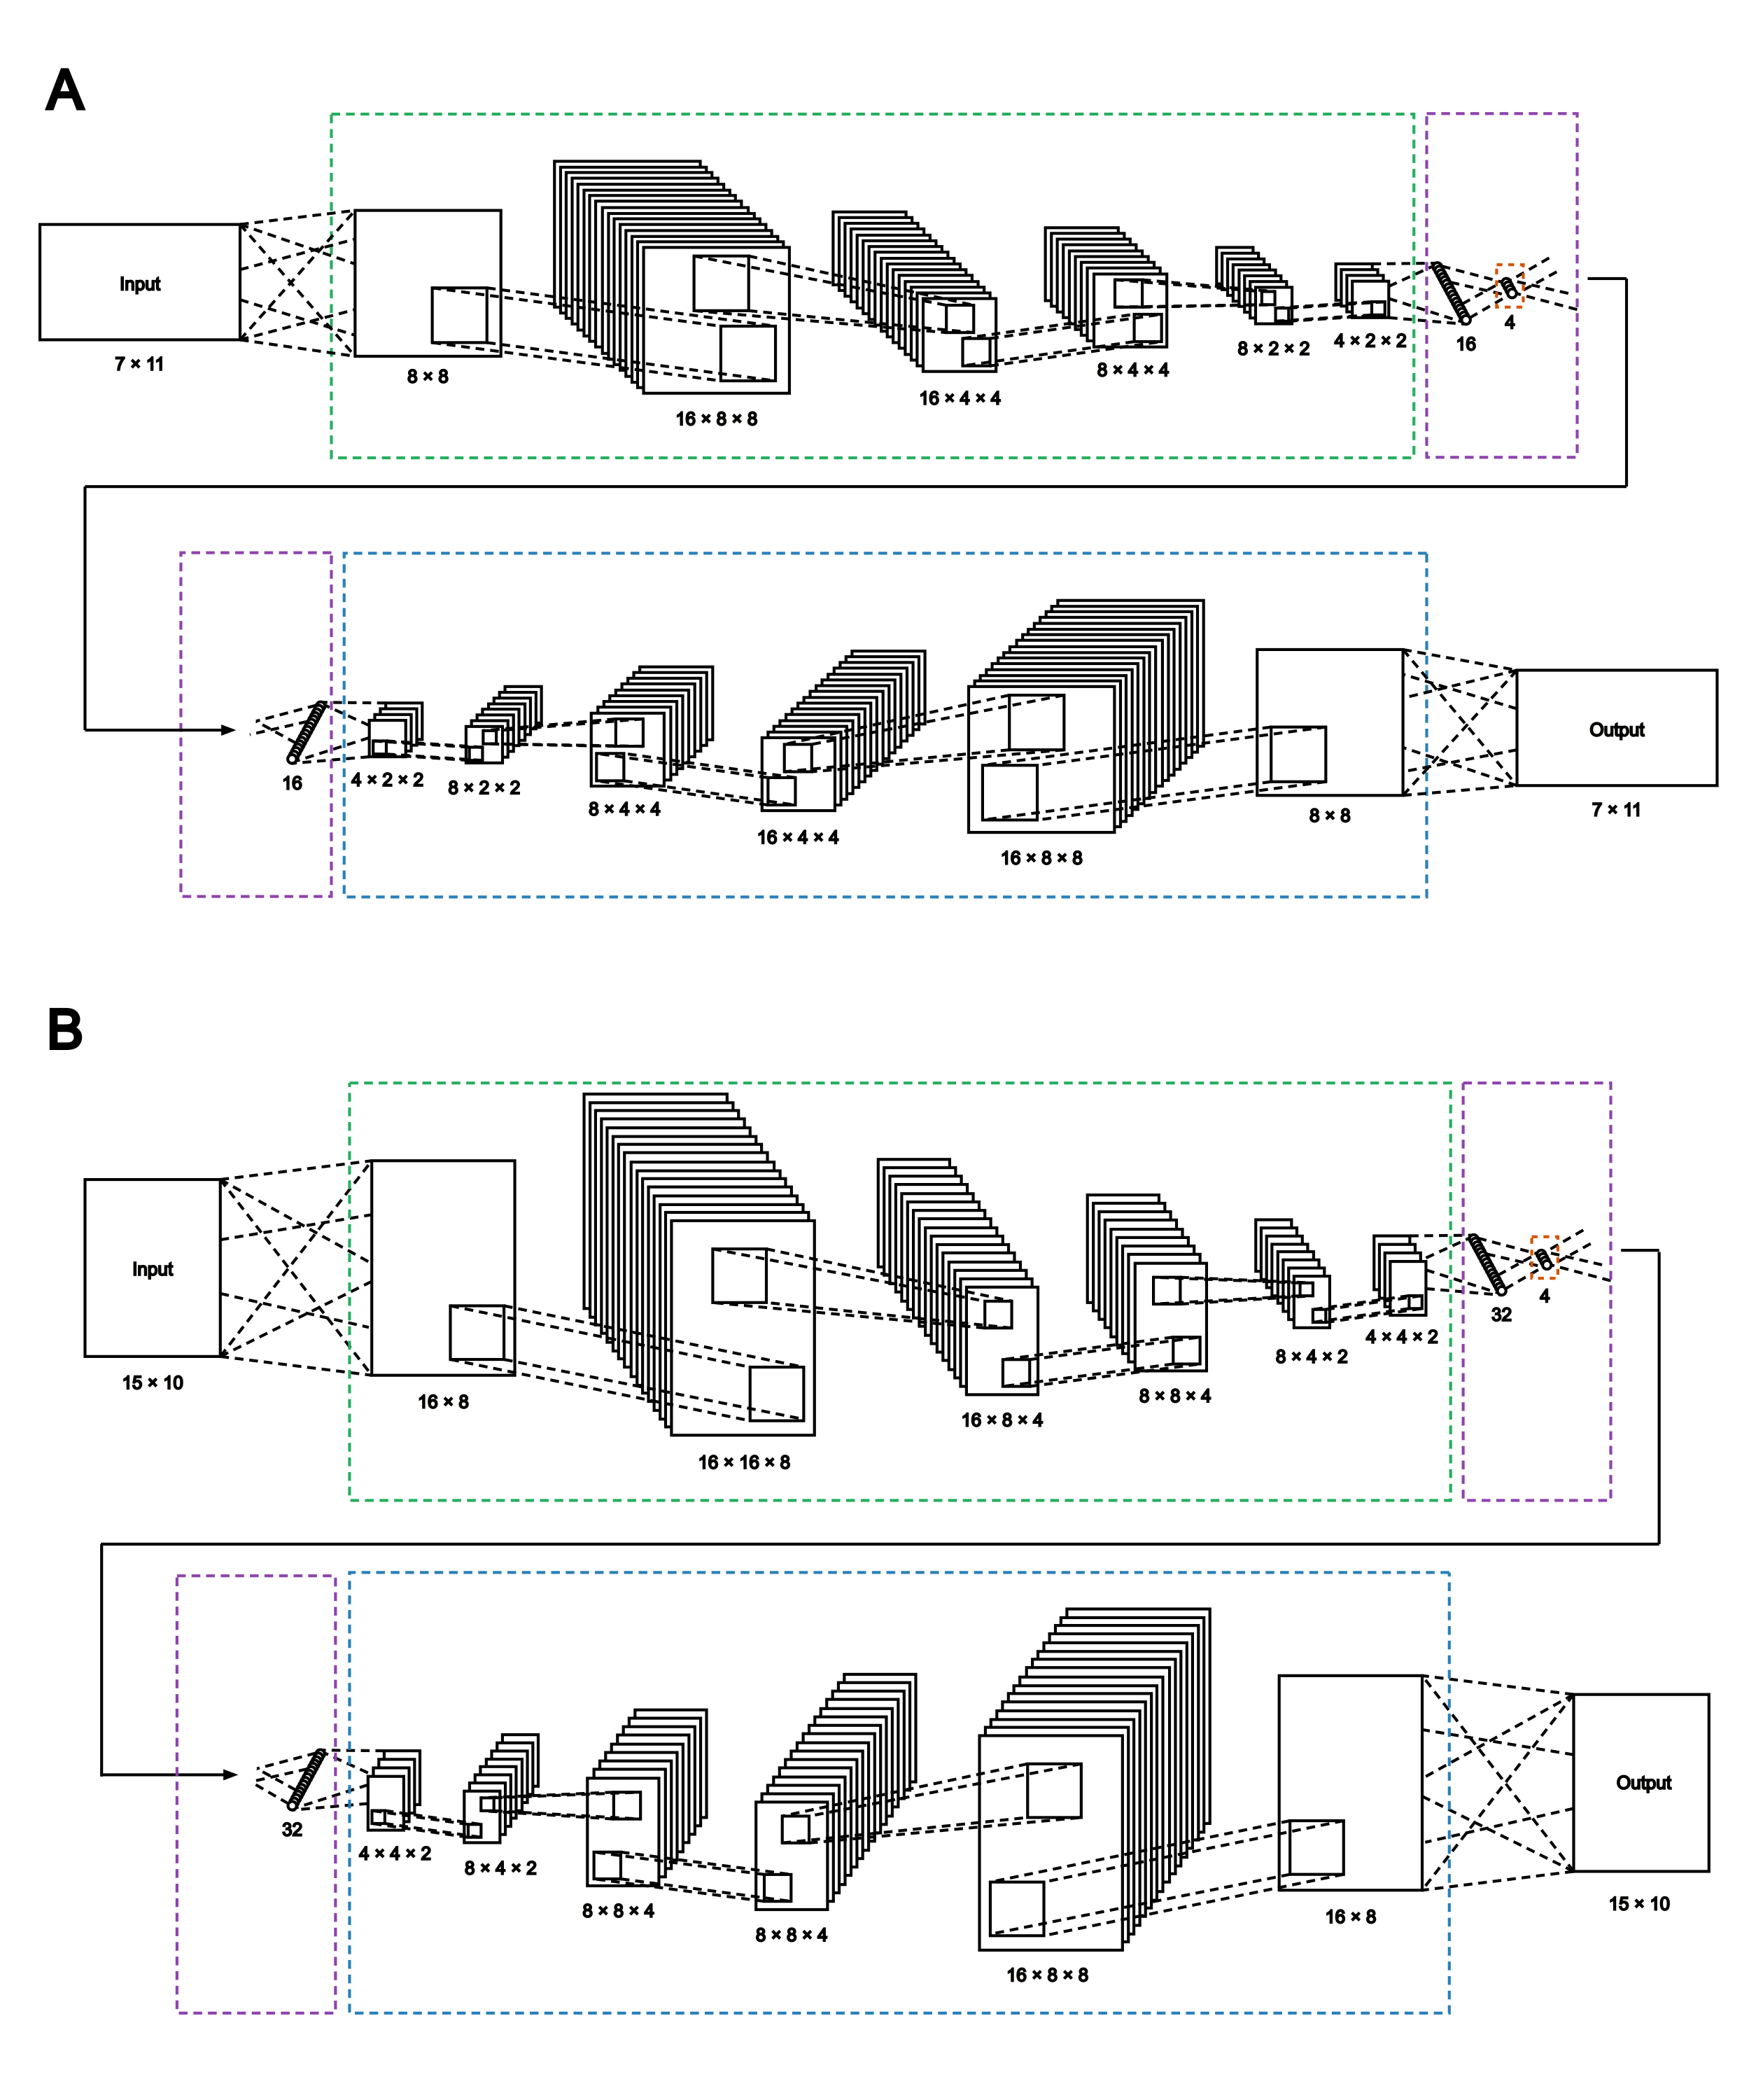
\includegraphics[width=0.9\columnwidth]{figures/CAE}
\caption{CAE architectures used for dimensionality reduction of the mouse (\textbf{A}) and human (\textbf{B}) datasets. Green sections indicate convolutional layers involved in the encoding process, and purple sections indicate the encoded dense (fully connected) network. Blue sections indicate layers involved in the decoding process. The layer indicated in orange is the four-dimensional layer that is extracted upon training. The dimensions of each layer are shown below the respective layer. \label{fig:CAE}%
}
\end{center}
\end{figure}

The four-dimensional encodings obtained from the CAE were then reduced to two dimensions using t-SNE, which attempts to retain high-dimensional features in a lower dimensions using probabilistic methods. According to  \cite{Maaten2008VisualizingDU}, t-SNE first computes the distance between points in a high-dimensional space by computing a conditional probability $p_{j|i}$ such that close points have a high probability whereas highly separated points have a near-zero probability. This probability is given by

$$p_{j|i}=\frac{exp(-||x_i-x_j||^2/2\sigma_i^2)}{\sum_{k\neq i}exp(-||x_i-x_k||^2/2\sigma_i^2)}.$$

\noindent
with $\sigma_{i}$ equal to the variance of an $x_{i}$-centered normal distribution. $||x||$ represents the second norm of vector $x$, or the Euclidean distance from the origin. The similarity $q_{j|i}$ between lower-dimensional points $y_i$ and $y_j$ obtained from applying a transformation to the original $x_i$ and $x_{j}$ is given instead by a Student's t distribution with a single degree of freedom such that

$$q_{j|i} = \frac{exp(1+||y_i-y_j||^2)^{-1}}{\sum_{k\neq i}exp(1+||y_k-y_i||^2)^{-1}}.$$

Similar to the objective function of a neural network, t-SNE seeks to iteratively minimize a cost function given by the difference between the original $p_{j|i}$ and the computed $q_{j|i}$. This is computed using the Kullback-Leibler divergence, which gives the difference between two probability distributions $P_{i}$ and $Q_{i}$ by computing the integral

$$\int_{-\infty}^{\infty}p_i(x) \log \frac{p_i(x)}{q_i(x)} dx$$

\noindent
for continuous probability distributions \citep{Bishoplearning}. In t-SNE, the objective function is computed by taking the sum of all Kullback-Leibler divergences over all points $i$ given by 

$$C=\sum_{i}\sum_{j}p_{i|j}\log \frac{p_{i|j}}{q_{i|j}}.$$

\noindent
Minimization of this cost function is also performed similar to the minimization of that of a neural network, using gradient descent. This gradient is given by

$$\frac{\partial C}{\partial y_i}=4\sum_{j}(p_{i|j}-q_{i|j})(y_i-y_j)(1+||y_i-y_j||^2)^{-1}$$

\noindent
and is updated with

$$\gamma^{(t)}=\gamma^{(t-1)}+\eta\frac{\partial C}{\partial \gamma}+\alpha(t)\left(\gamma^{(t-1)}-\gamma^{(t-2)}\right)$$

\noindent
where $\gamma^{(t)}$ is the solution at time $t$, $\eta$ is the learning rate, and $\alpha(t)$ is the momentum at $t$. 
\subsection{Cluster identification}

Once each dataset was reduced to two dimensions, the density-based spatial clustering of applications with noise (DBSCAN) algorithm was applied to label clusters of similar gene expression. Unlike partitioning-based clustering, which attempts to find a function that best separates classes of points, or hierarchical clustering, which iteratively builds larger and larger clusters, DBSCAN is instead based on detecting dense collections of points. DBSCAN has many benefits, the most notable of which are high outlier robustness and noise detection ability. In addition, unlike many other algorithms, there is no need to manually input $k$, the hyperparameter that denotes the number of desired clusters \citep{Ester1996ADA}.

\subsection{Clustering comparison}

Clusters were compared by computing the adjusted rand index (ARI) which provides an indication of the similarity between two clusterings while taking into account results explained by random variance. The ARI returns a value between 0 and 1, with 0 indicating a clustering that may be the result of pure chance and 1 indicating that the two clusterings are completely identical. The ARI is a symmetric measure, meaning that the order of the two clusters does not matter in calculation. The ARI is computed by constructing a contingency matrix between two clusterings $k$ and $h$ with $C$ and $R$ elements,respectively, such that each entry $n_{ij}$ denotes the intersection between cluster $i$ of $k$ and cluster $j$ of $h$ (Table~\ref{table:2}). 

\begin{table}[H]
\begin{center}
\caption{The contingency matrix used in computing the ARI between two clusterings $k$ and $h$. \citep{Zhang2010ARImpAG}}
\begin{tabular}{ l | l l l l l | l } 
Cluster	& $k_1$ & $k_2$ & $k_3$ & $\cdots$ & $k_C$ & $\sum$ \\ 
\hline
$h_1$ & $n_{11}$ & $n_{12}$ & $n_{13}$ & $\cdots$ & $n_{1C}$ & $N_{1.}$\\ 
$h_{2}$ & $n_{21}$ & $n_{22}$ & $n_{23}$ & $\cdots$ & $n_{2C}$ & $N_{2.}$\\ 
$h_{3}$ & $n_{31}$ & $n_{32}$ & $n_{33}$ & $\cdots$ & $n_{3C}$ & $N_{3.}$\\ 
$\vdots$ & $\vdots$ & $\vdots$ & $\vdots$ & $\ddots$ & $\vdots$ & $\vdots$\\ 
$h_{R}$ & $n_{R1}$ & $n_{R2}$ & $n_{R3}$ & $\cdots$ & $n_{RC}$ & $N_{R.}$\\ 
\hline
$\sum$ & $N_{.1}$ & $N_{.2}$ & $N_{.3}$ & $\cdots$ & $N_{.C}$ & $N$\\ 
\end{tabular}
\label{table:2}
\end{center}
\end{table}

\noindent
The ARI may be computed \citep{Yeung2001DetailsOT} through the sums

$$\frac{\sum_{i,j}{{n_{ij}}\choose{2}}-\frac{\left[\sum_{i}{{n_{i.}}\choose{2}}\sum_{j}{{n_{.j}}\choose{2}}\right]}{{n\choose{2}}}}{\frac{1}{2}\left[\sum_{i}{{n_{i.}}\choose{2}}+\sum_{j}{{n_{.j}}\choose{2}}\right]-\frac{\left[\sum_{i}{{n_{i.}}\choose{2}}\sum_{j}{{n_{.j}}\choose{2}}\right]}{{n\choose{2}}}}$$

\noindent
which are derived using the general hypergeometric distribution for significance.

\section{Results}

\subsection{Correlation clustering}

\begin{figure}[H]
\begin{center}
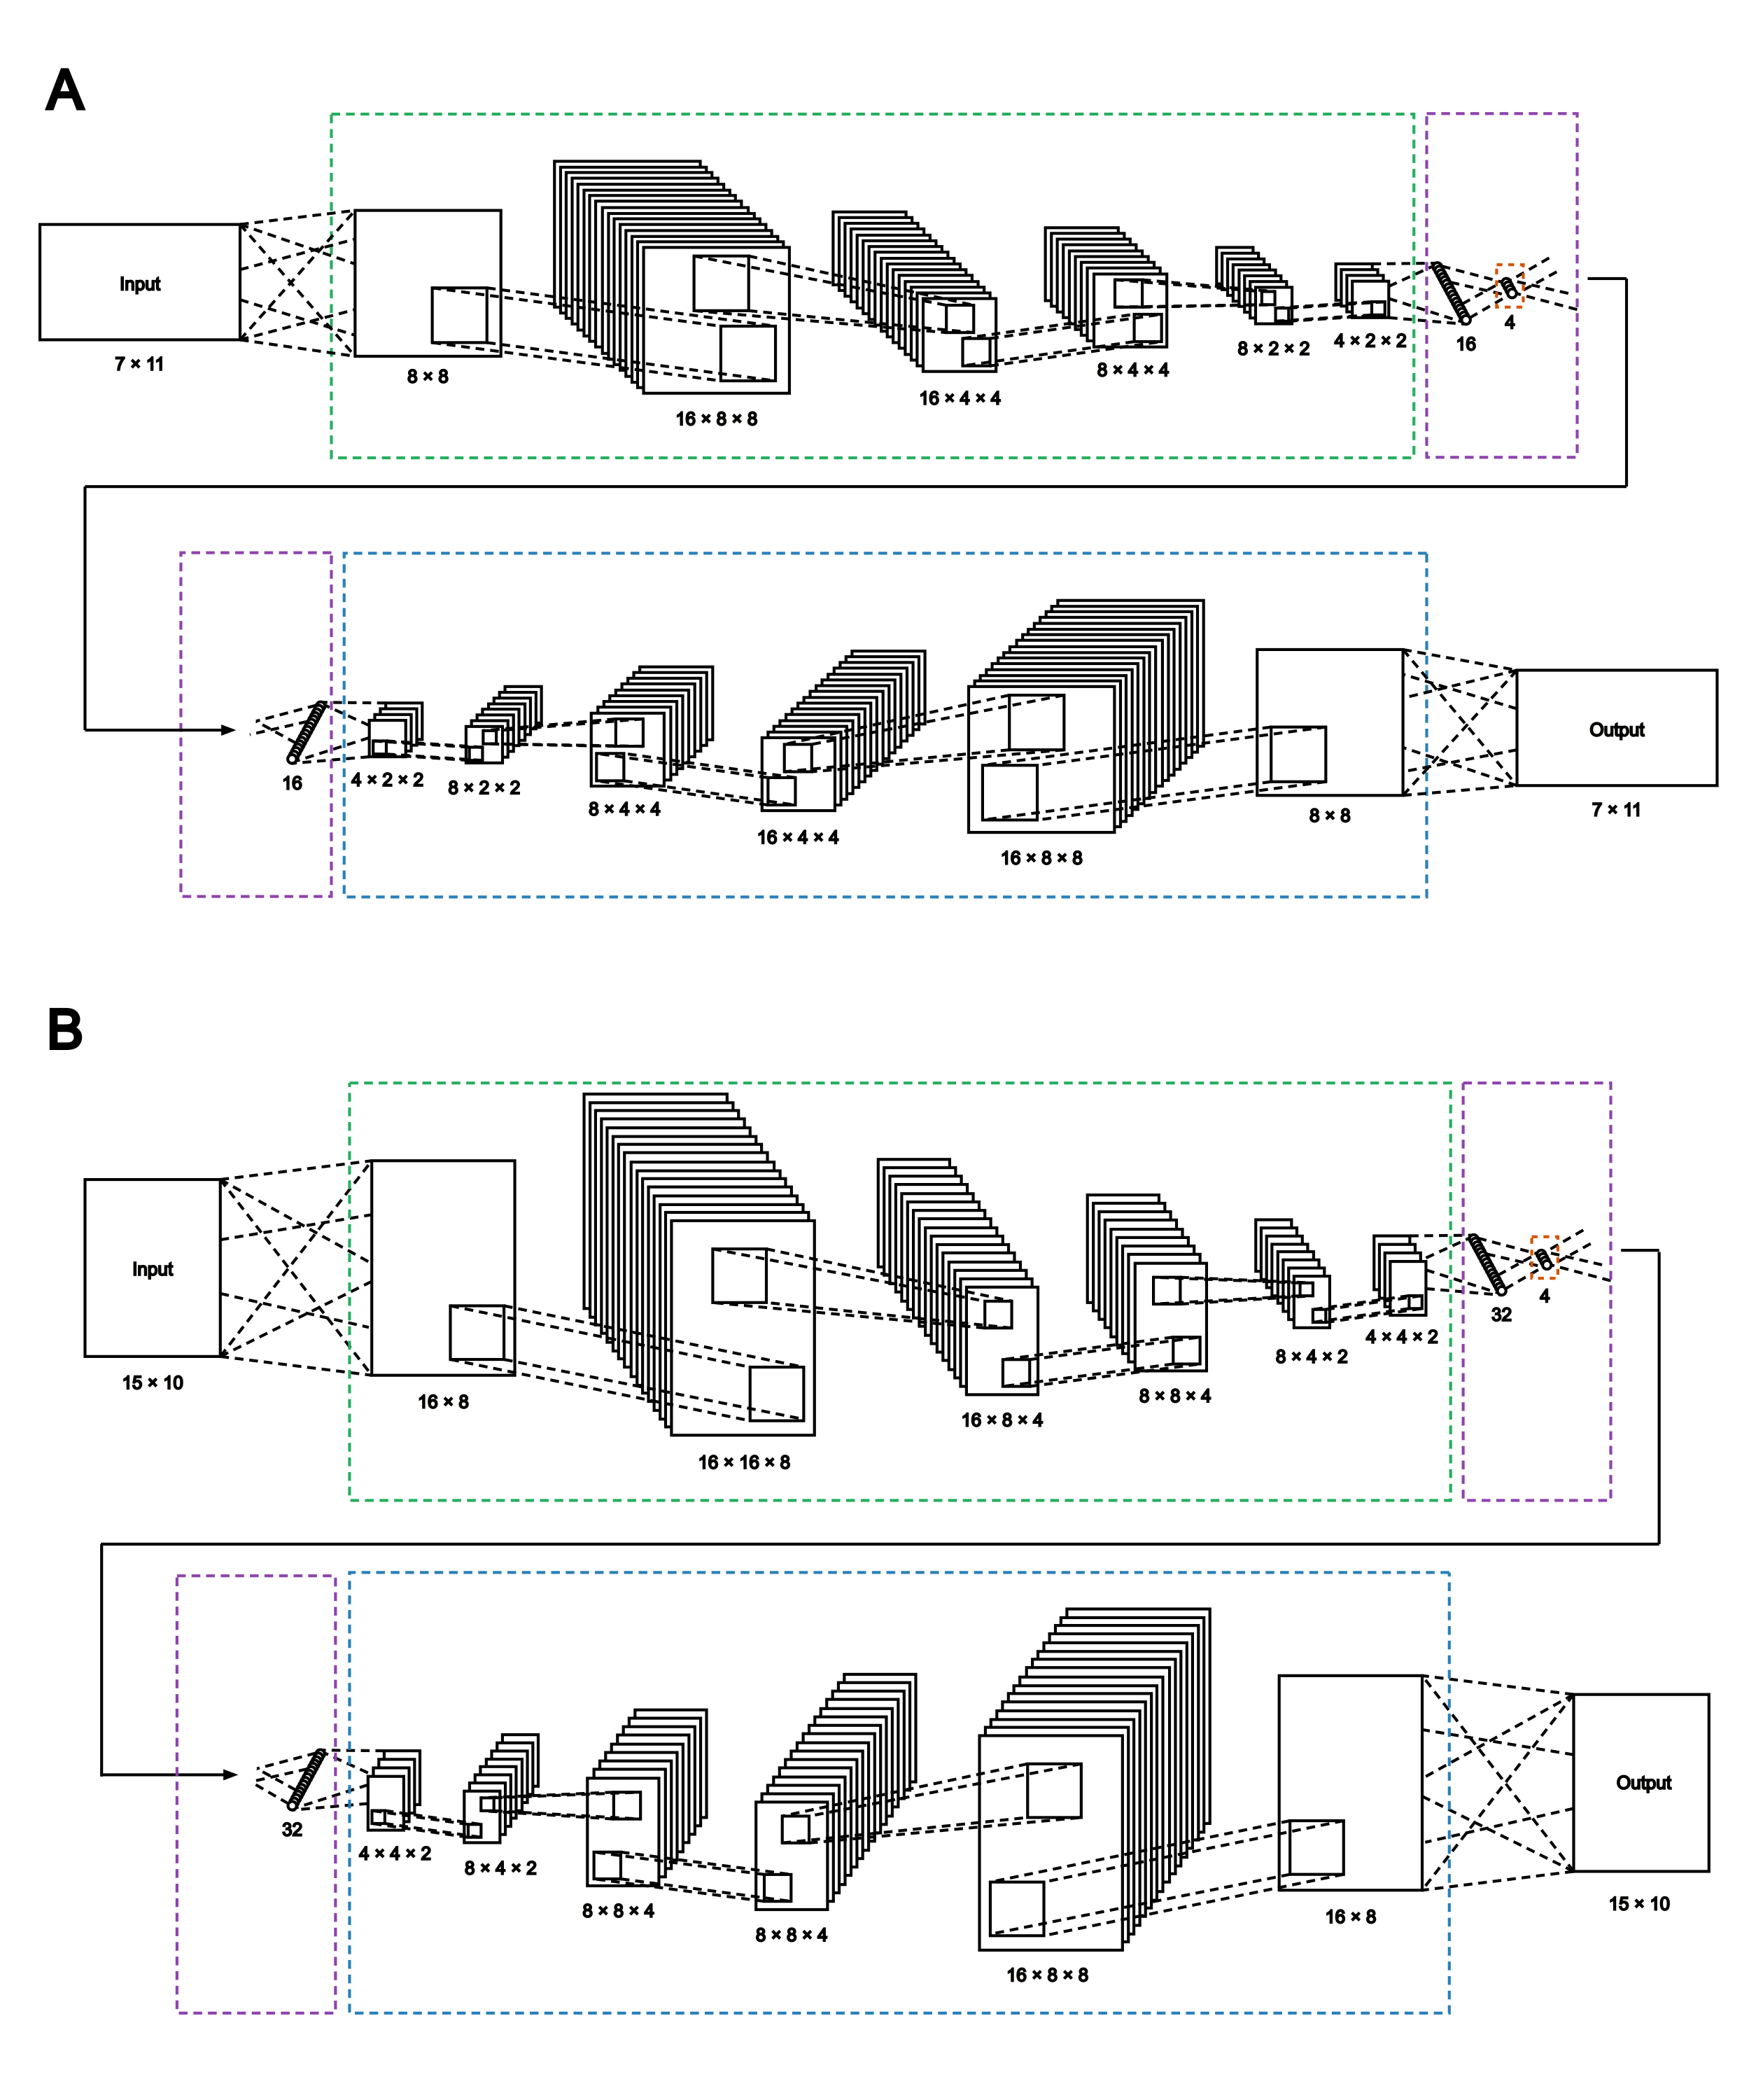
\includegraphics[width=0.9\columnwidth]{figures/CAE}
\caption{Correlation matrices produced using the Pearson's $r$ and Spearman $\rho$ measures. \label{fig:correlations}%
}
\end{center}
\end{figure}

\begin{figure}[H]
\begin{center}
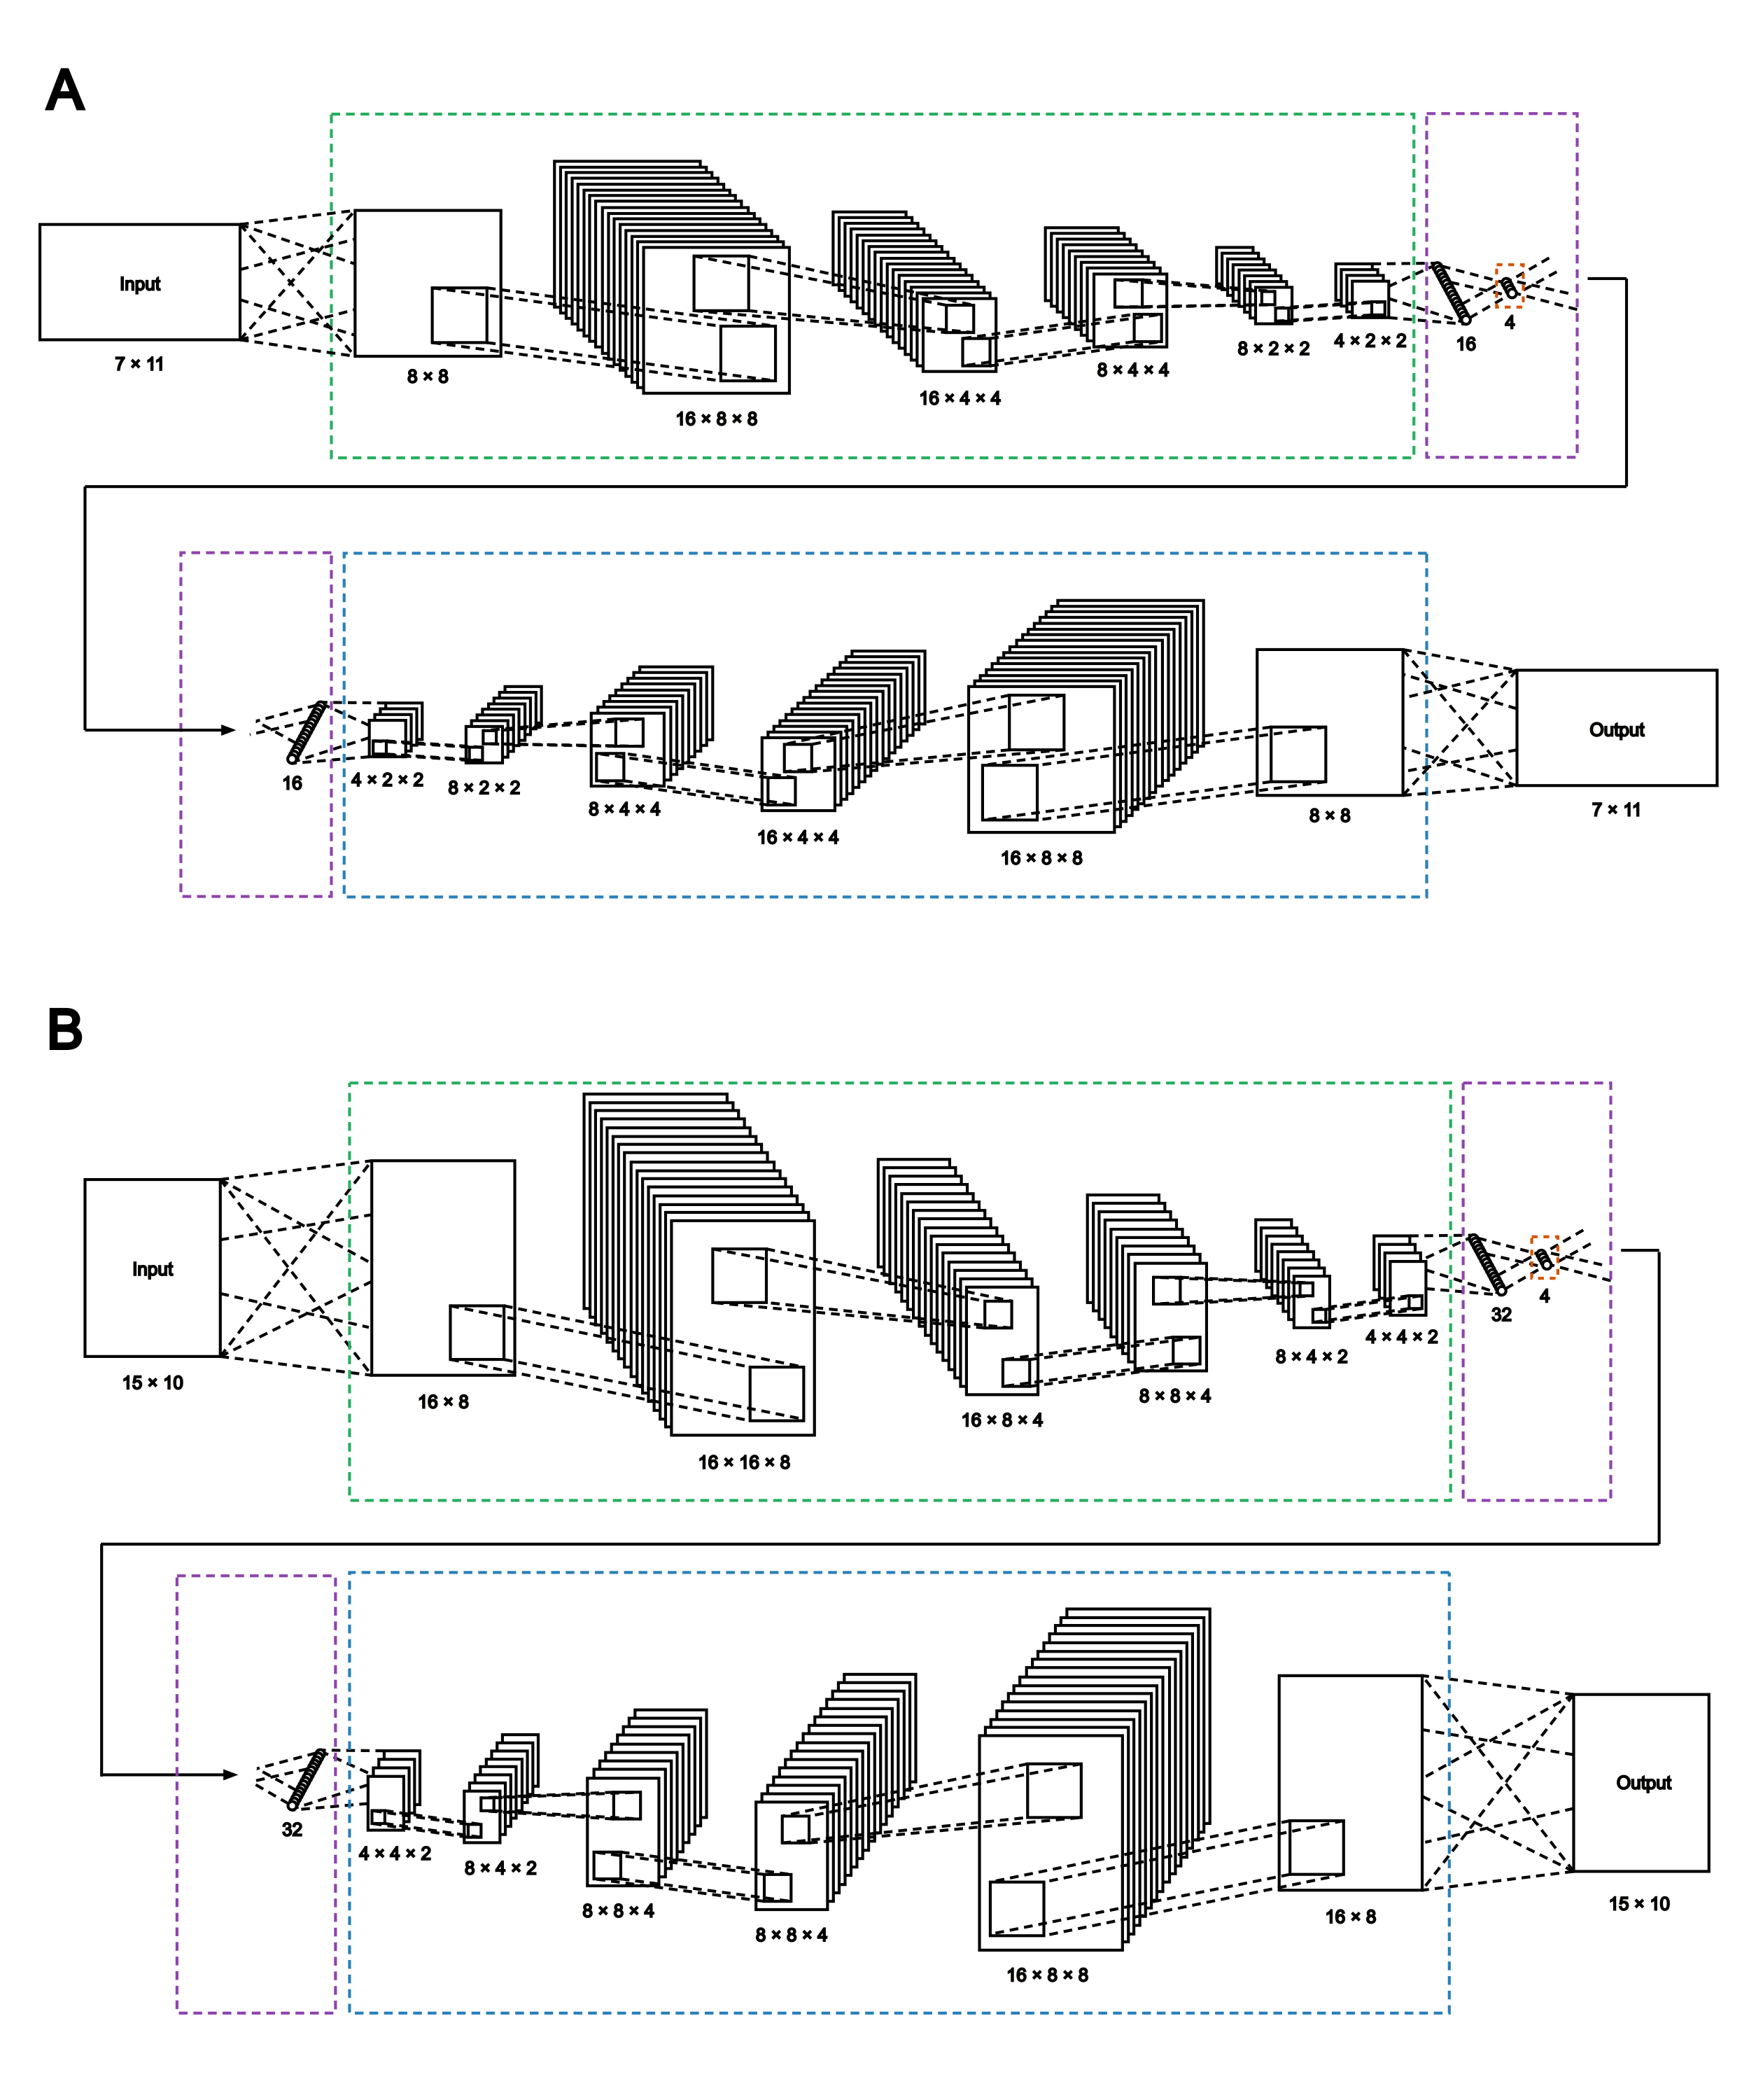
\includegraphics[width=0.9\columnwidth]{figures/CAE}
\caption{A force-based layout of the correlation relationships between genes computed using the ForceAtlas2 algorithm developed by \cite{Jacomy2014ForceAtlas2AC}. \label{fig:network}%
}
\end{center}
\end{figure}

\subsection{CAE-based encoding}

\begin{figure}[H]
\begin{center}
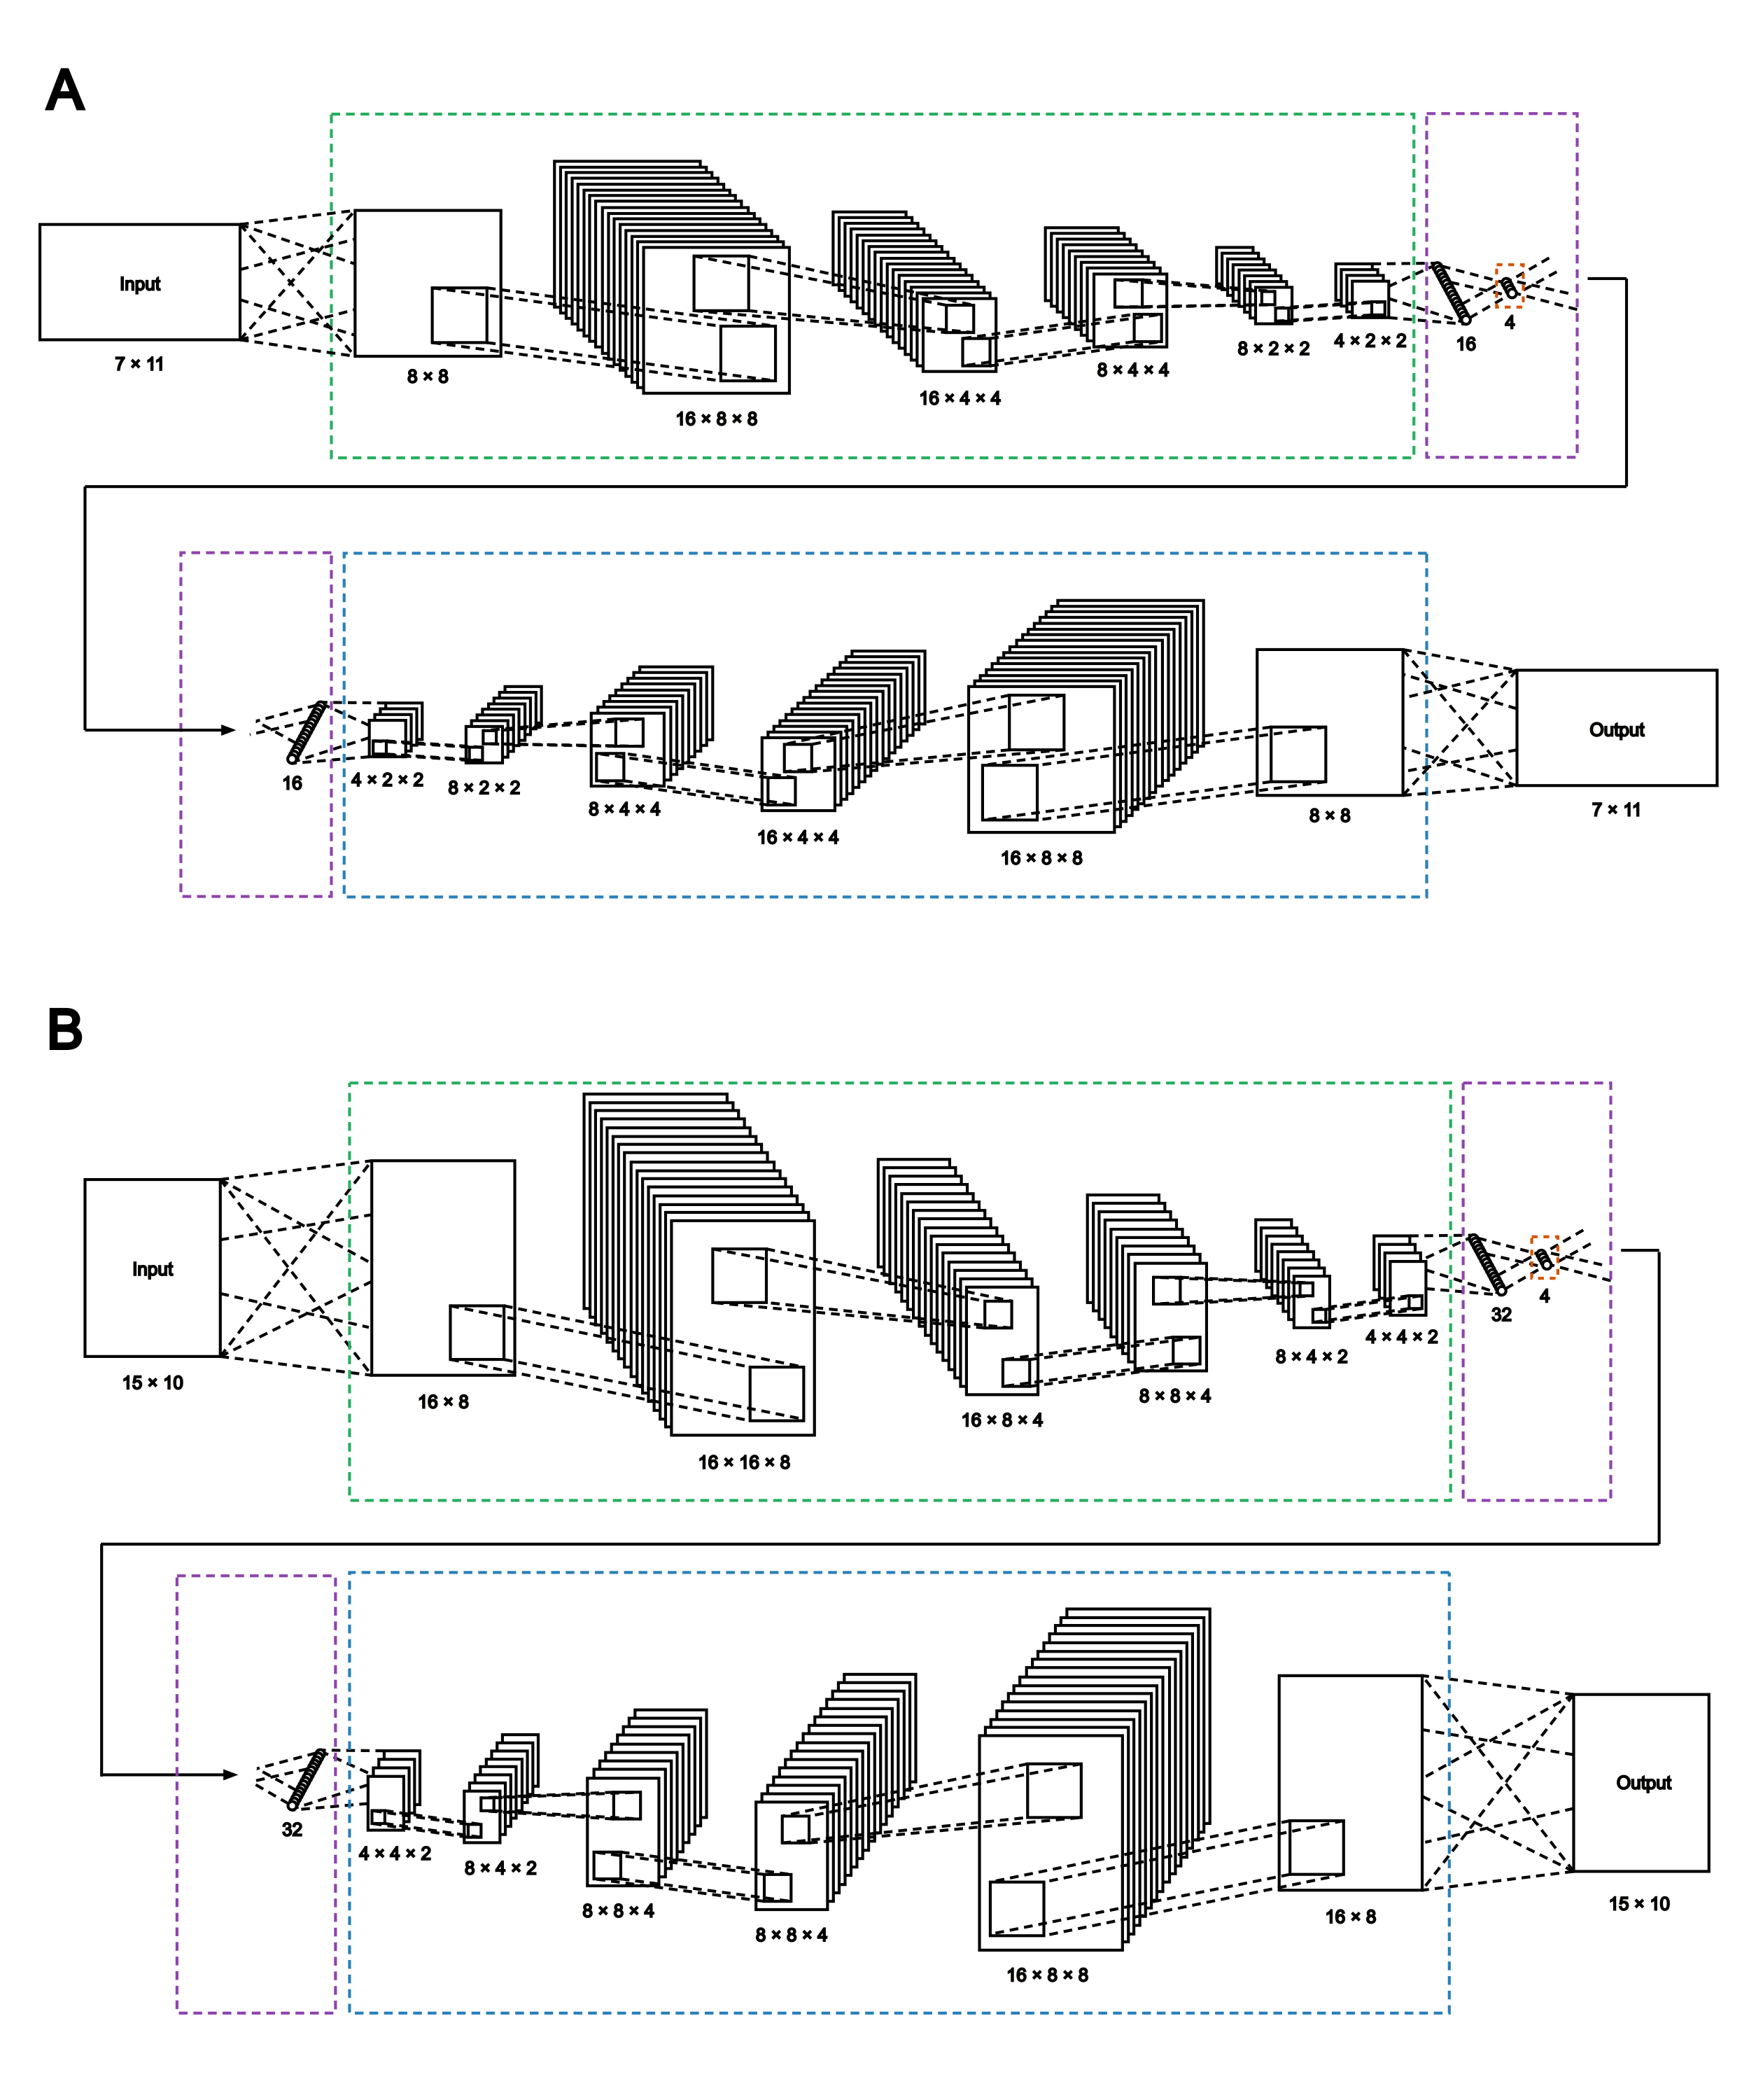
\includegraphics[width=0.9\columnwidth]{figures/CAE}
\caption{The loss curve with respect to time. \label{fig:rmse}%
}
\end{center}
\end{figure}

\begin{figure}[H]
\begin{center}
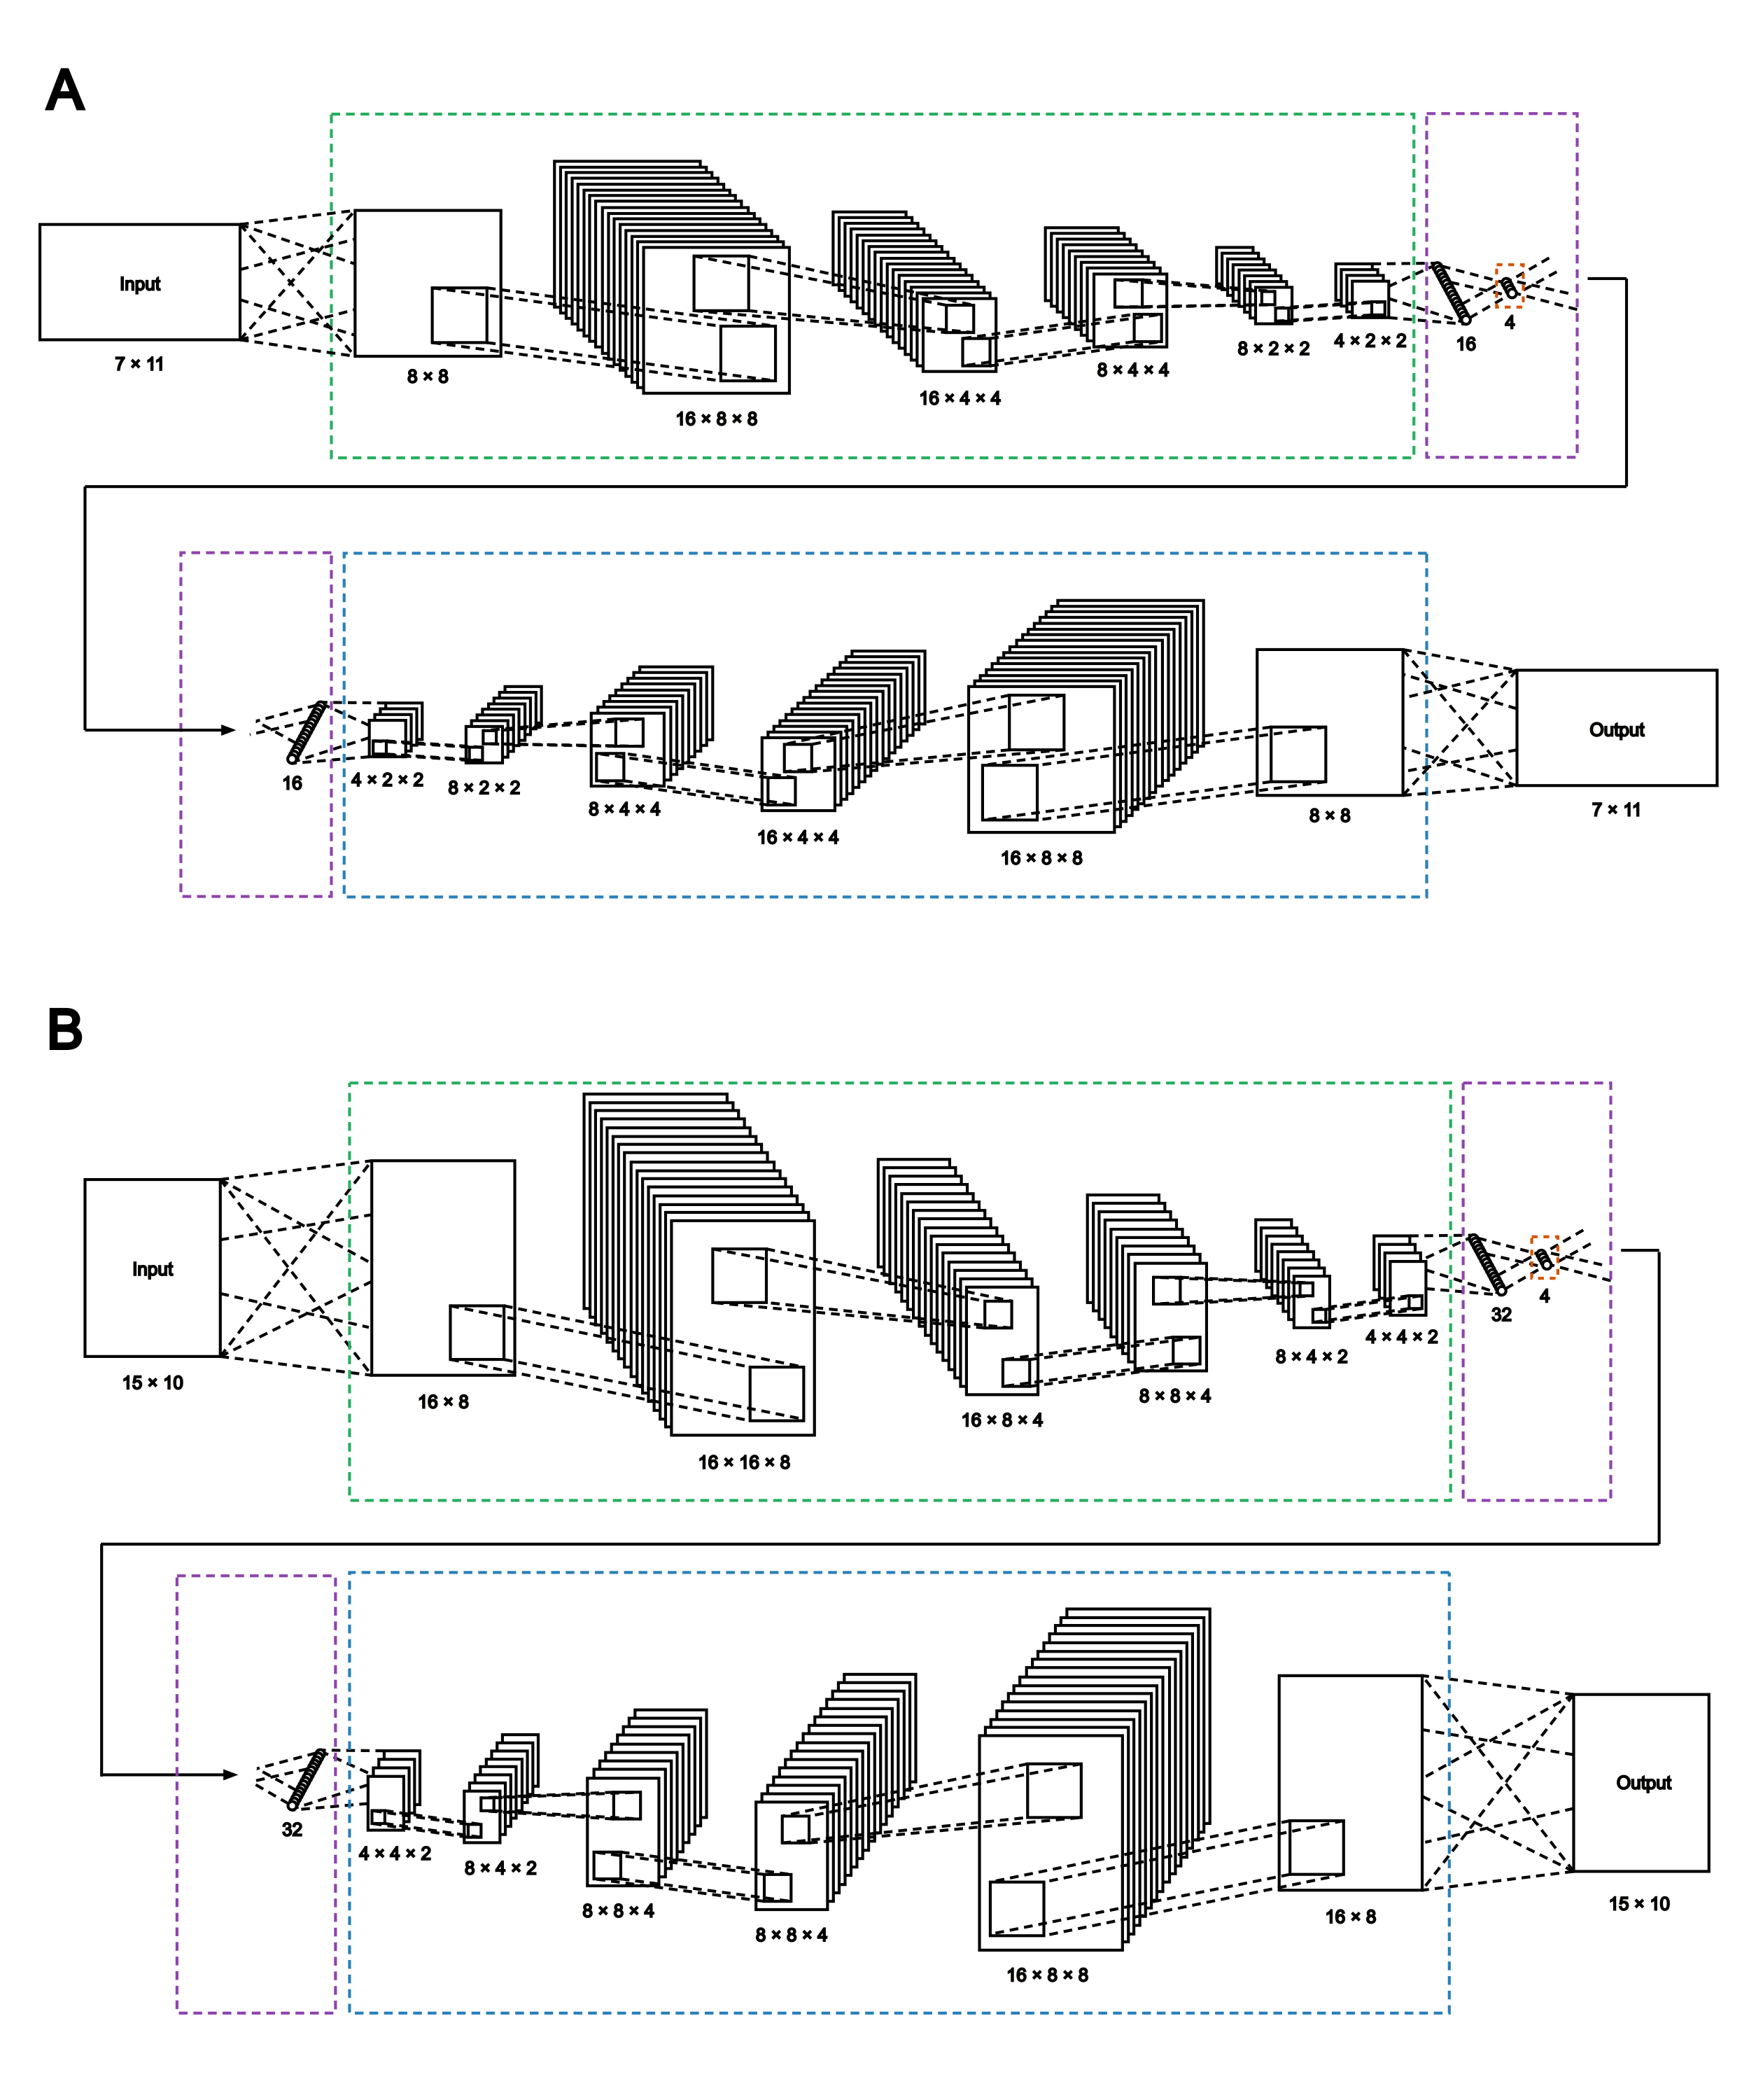
\includegraphics[width=0.9\columnwidth]{figures/CAE}
\caption{Comparison of CAE inputs and output expression profiles. \label{fig:input_output}%
}
\end{center}
\end{figure}

\subsection{t-SNE}

\begin{figure}[H]
\begin{center}
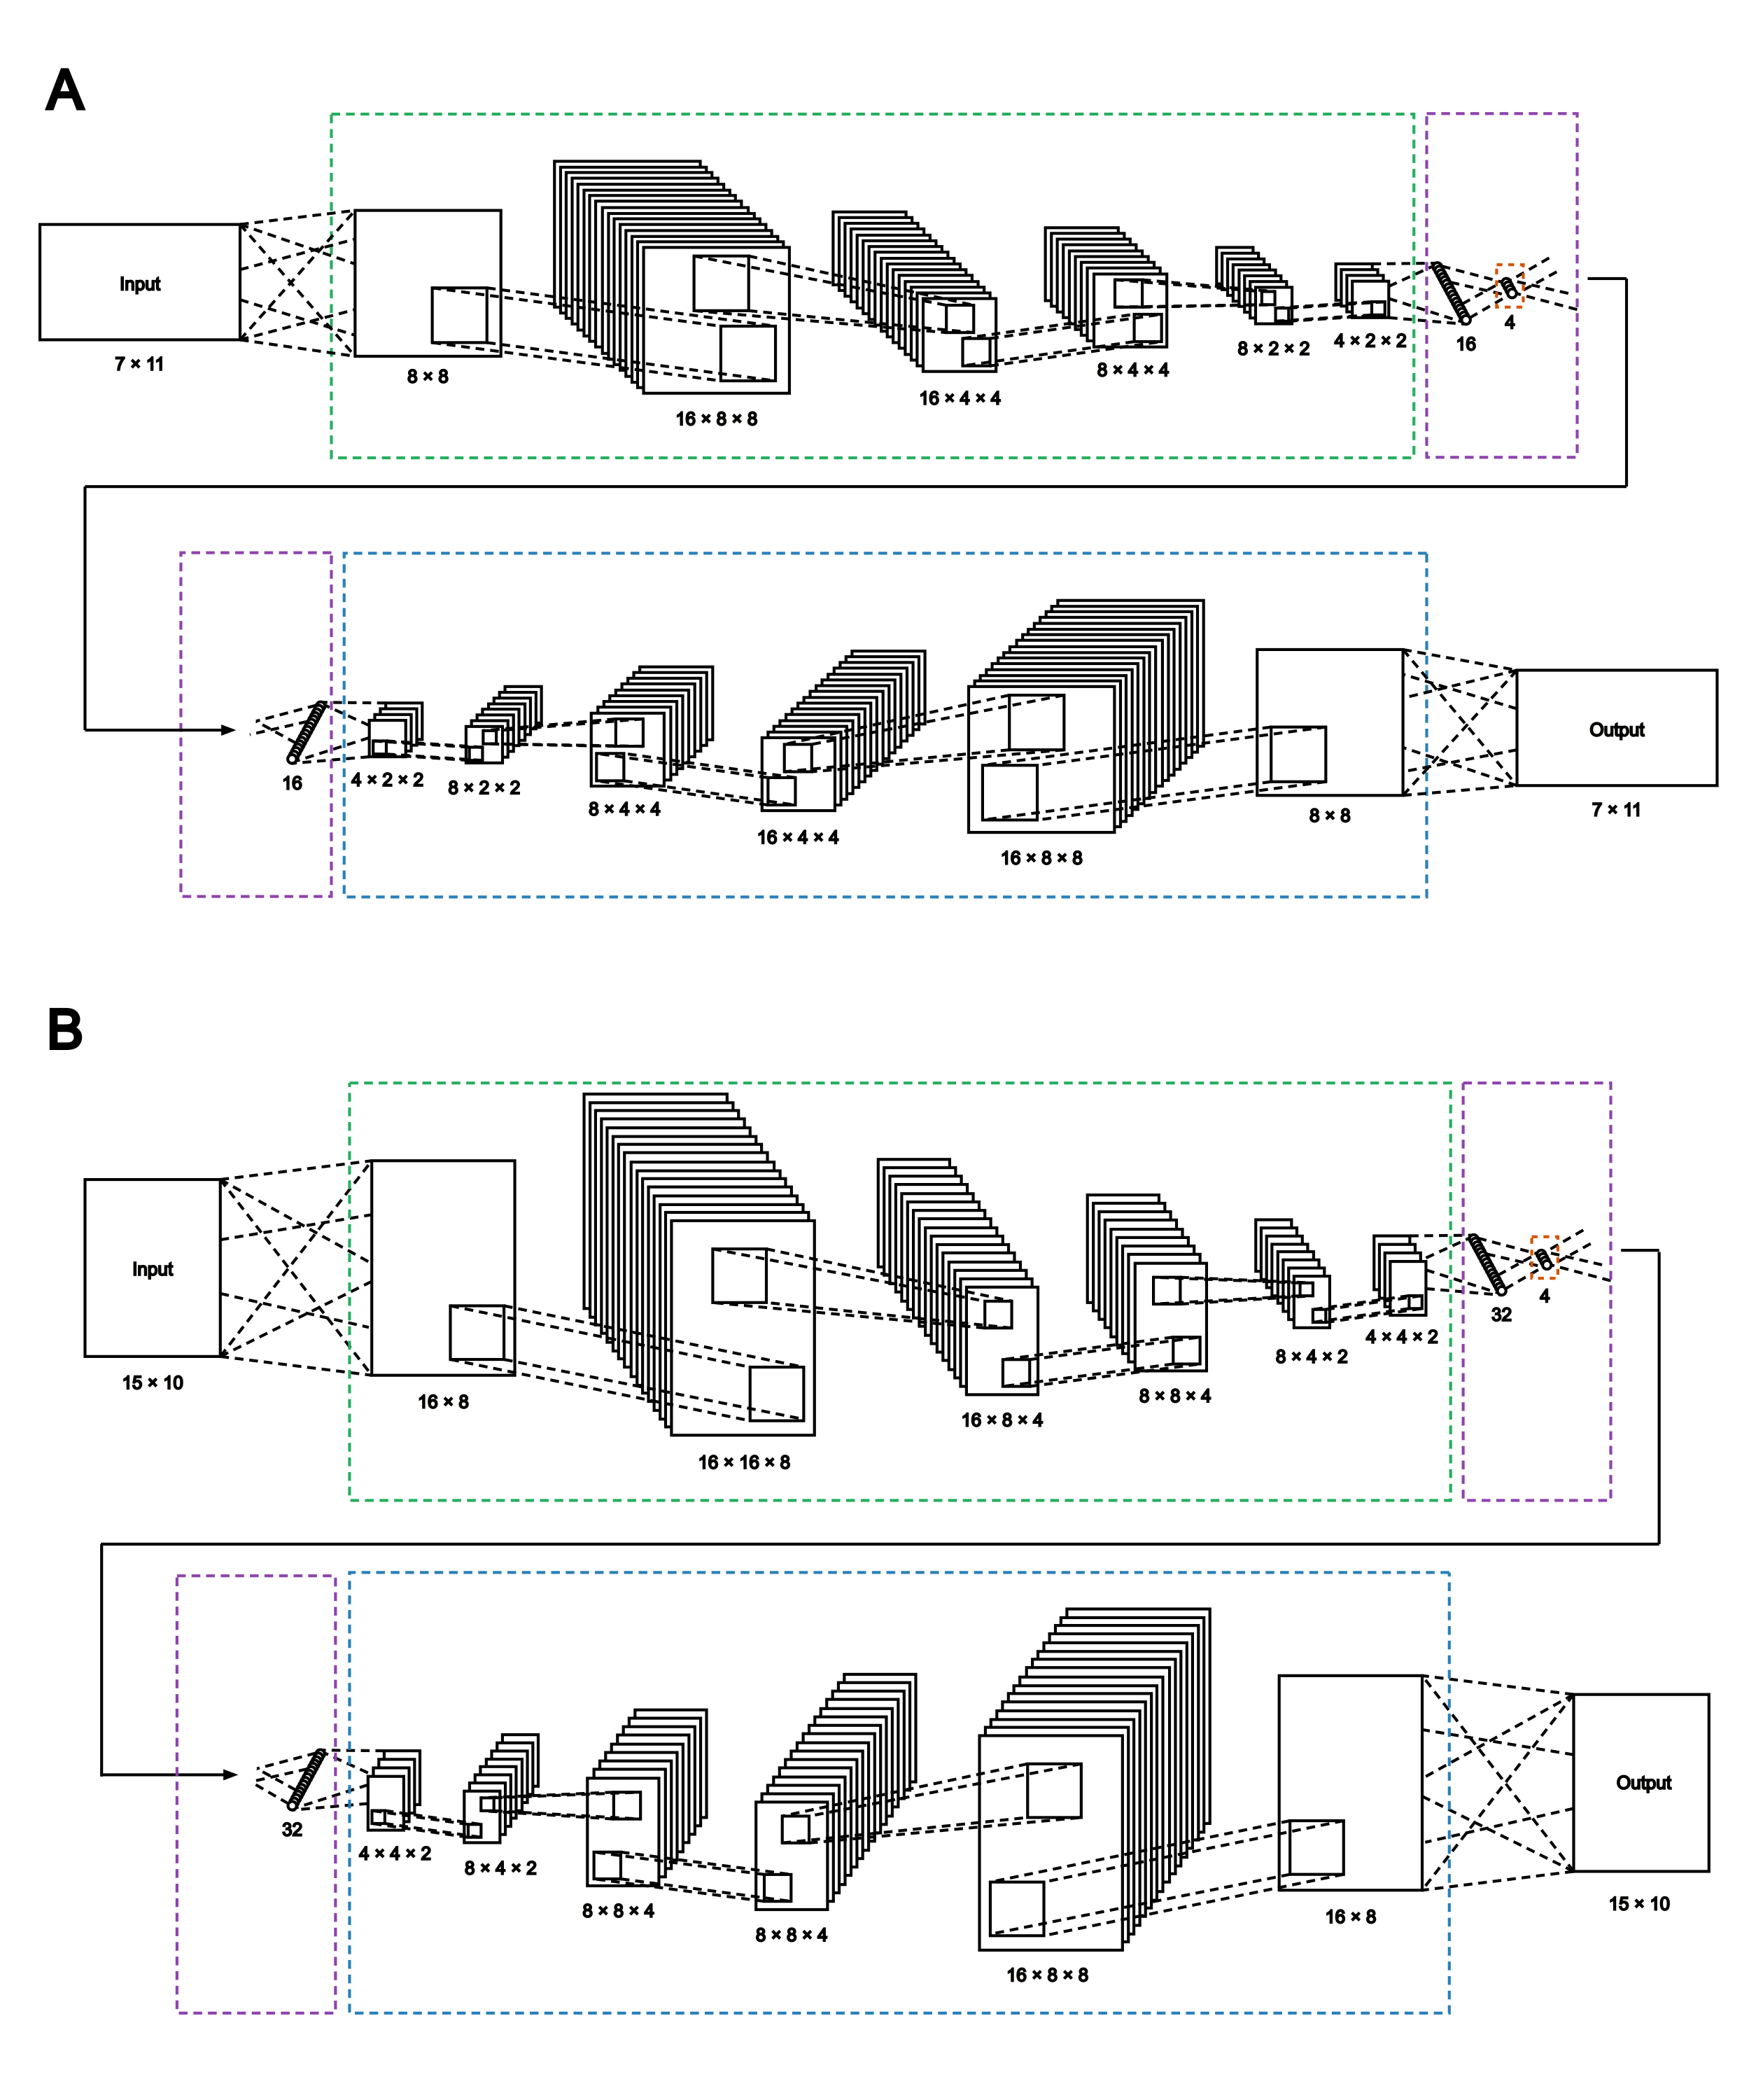
\includegraphics[width=0.9\columnwidth]{figures/CAE}
\caption{The two-dimensional representation returned by t-SNE. \label{fig:tsne_scatter}%
}
\end{center}
\end{figure}

\begin{figure}[H]
\begin{center}
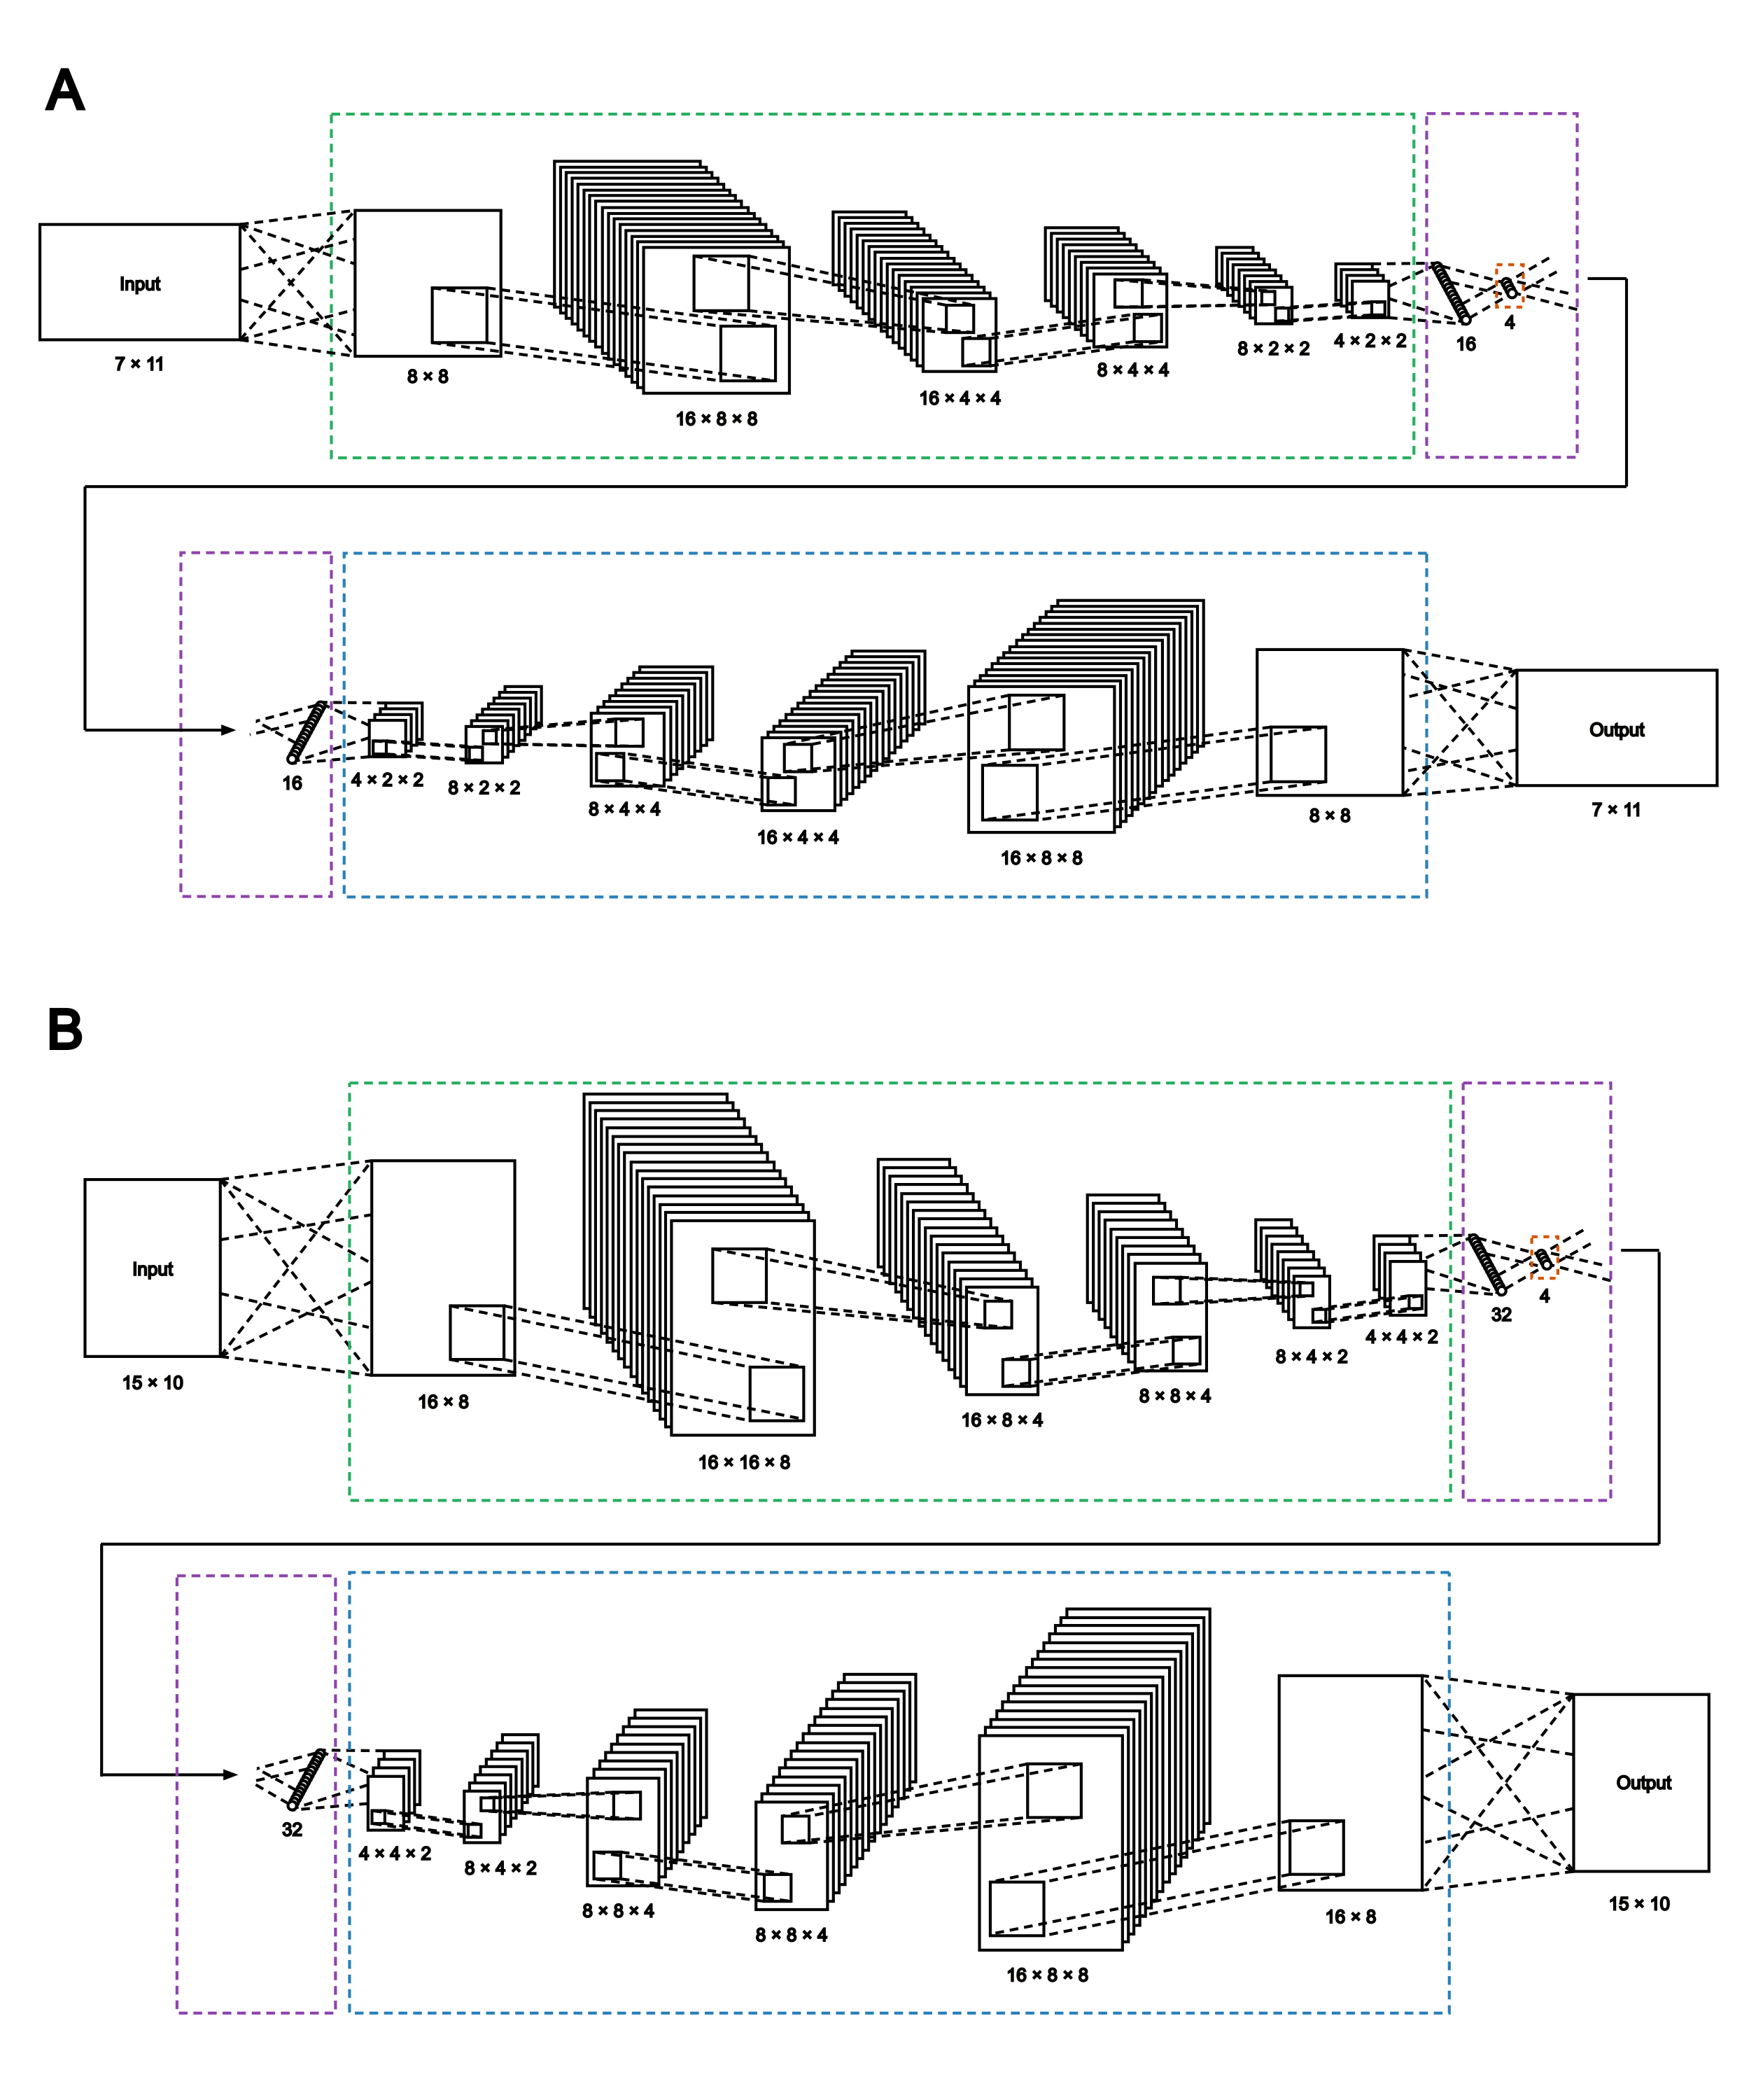
\includegraphics[width=0.9\columnwidth]{figures/CAE}
\caption{Representation of each point in the t-SNE output as the original image. \label{fig:image_scatter}%
}
\end{center}
\end{figure}

\begin{figure}[H]
\begin{center}
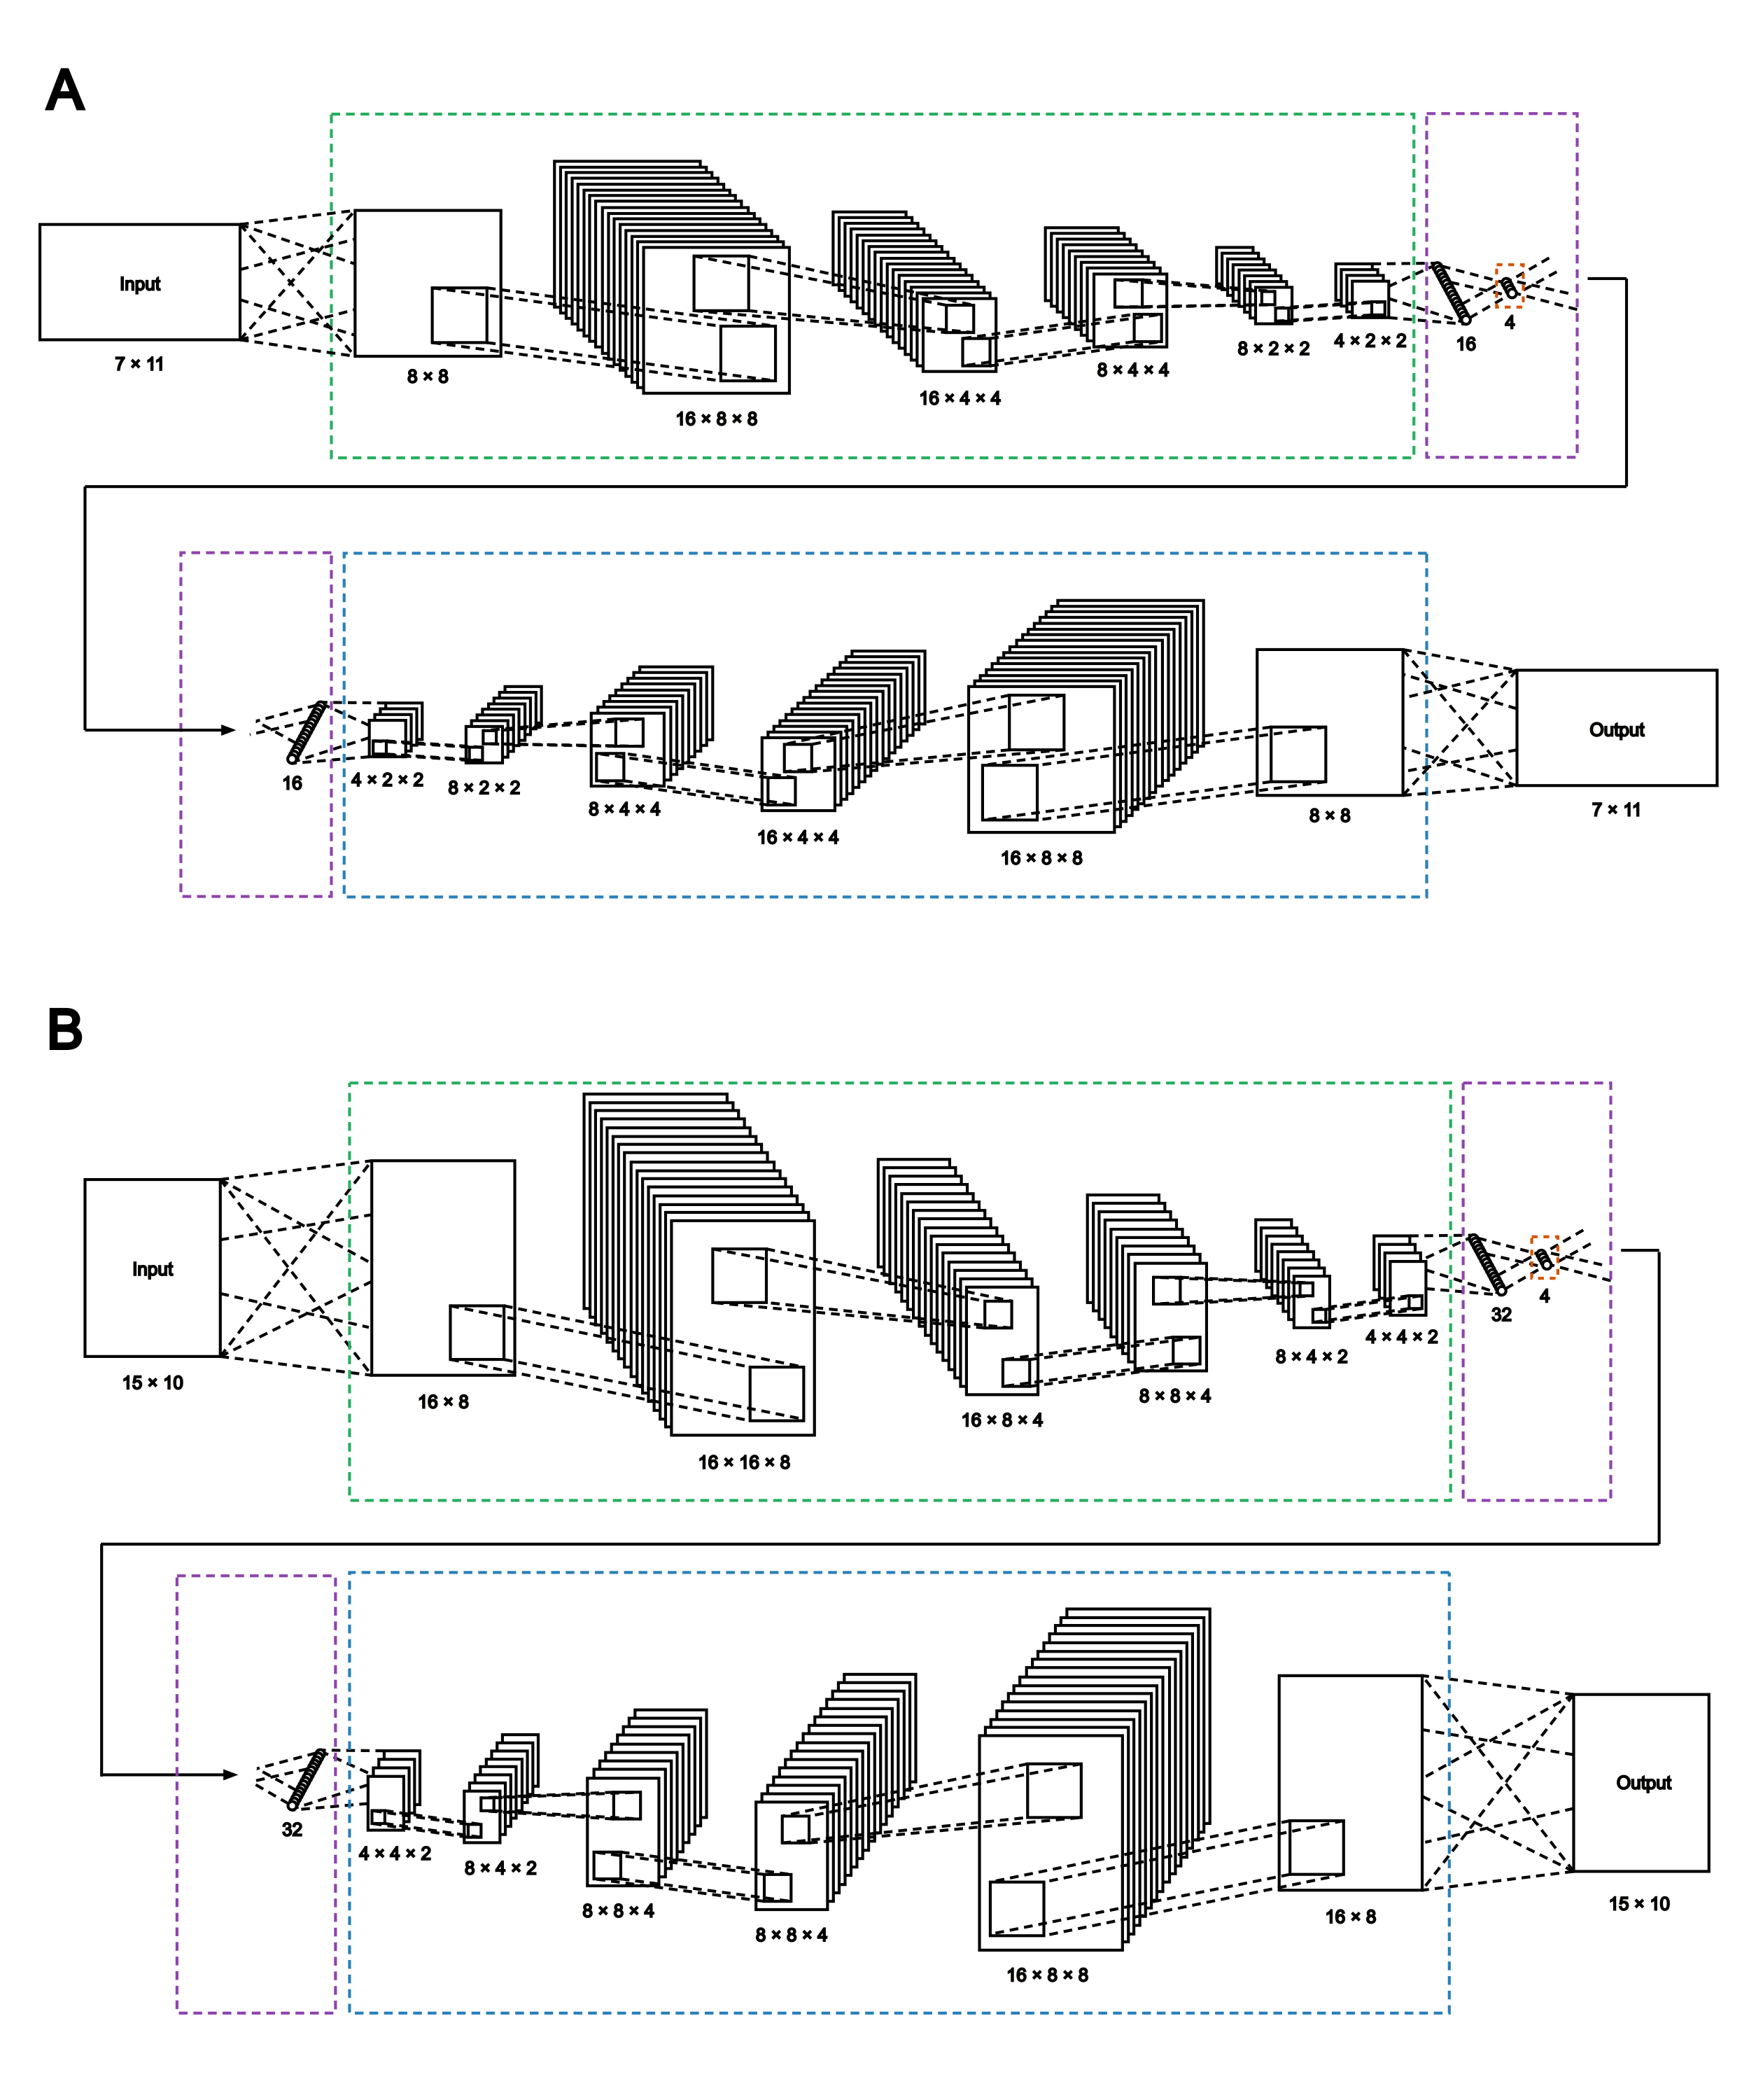
\includegraphics[width=0.9\columnwidth]{figures/CAE}
\caption{Comparison of raw correlation matrix and Euclidean distance matrix. \label{fig:new_matrix}%
}
\end{center}
\end{figure}

\subsection{Clustering}

\begin{figure}[H]
\begin{center}
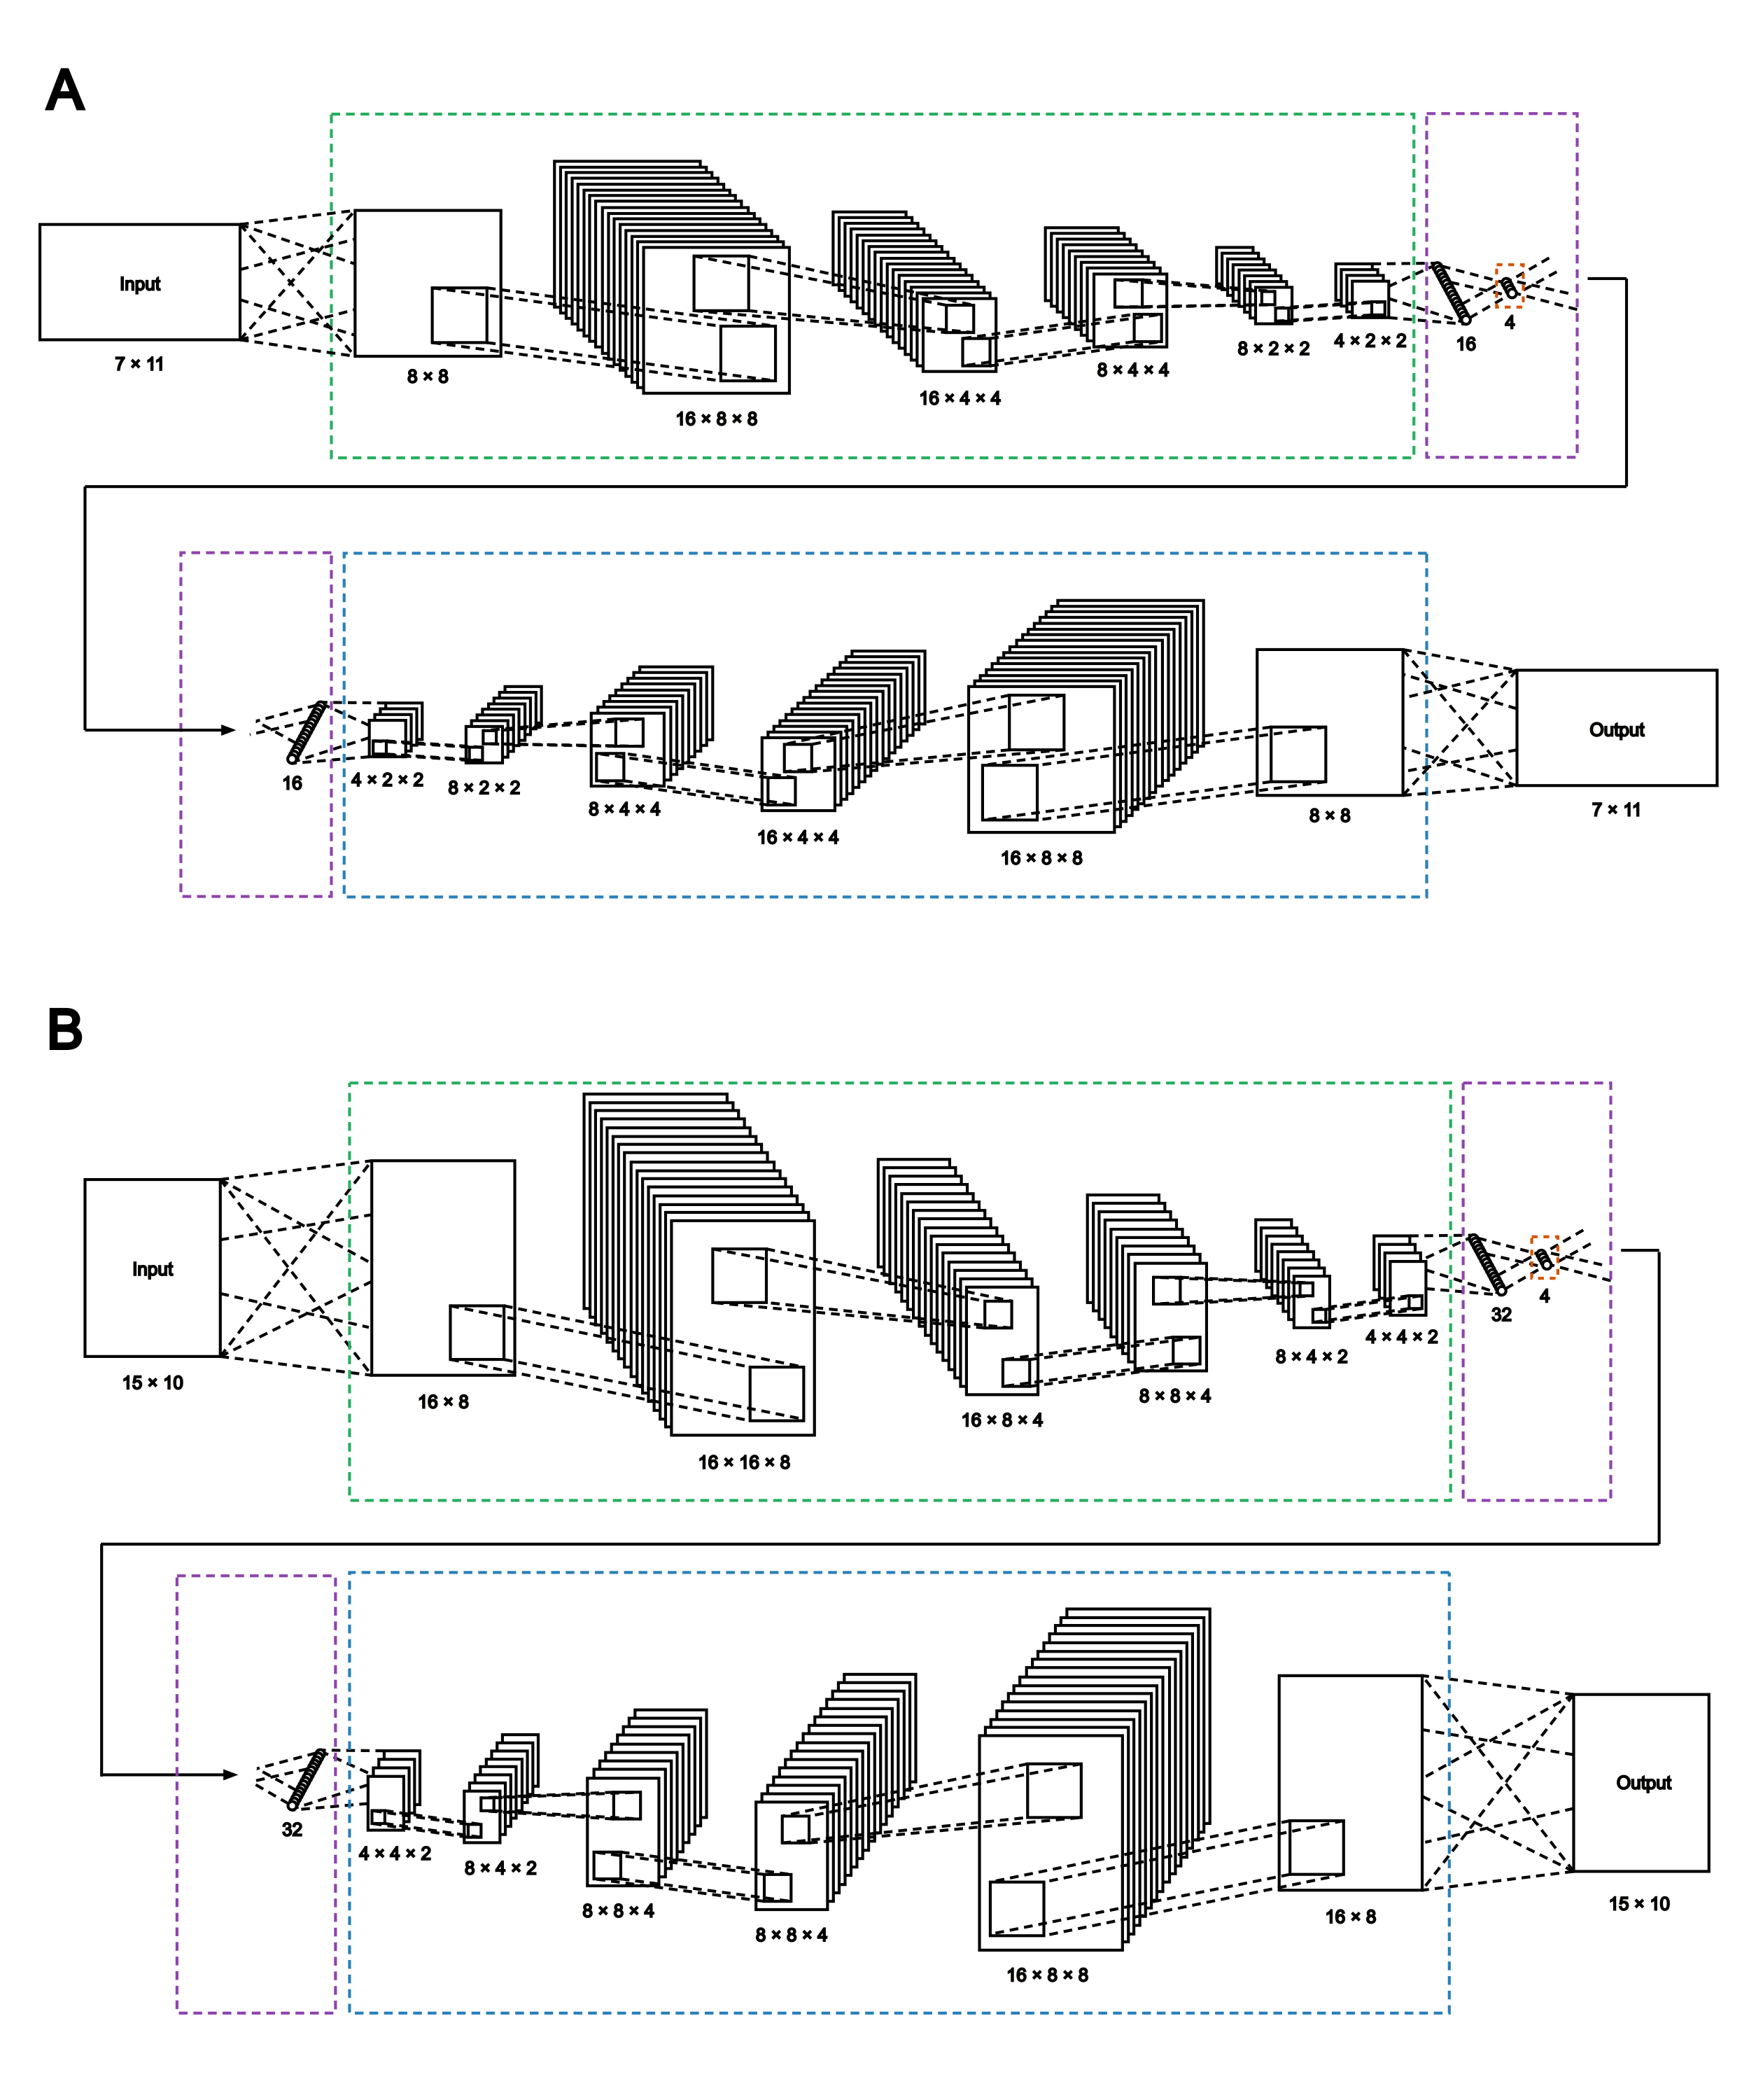
\includegraphics[width=0.9\columnwidth]{figures/CAE}
\caption{Coloring of clusters using DBSCAN. \label{fig:DBSCAN}%
}
\end{center}
\end{figure}

\subsection{Comparison}

% SHOULD ACTUALLY BE A TABLE
\begin{figure}[H]
\begin{center}
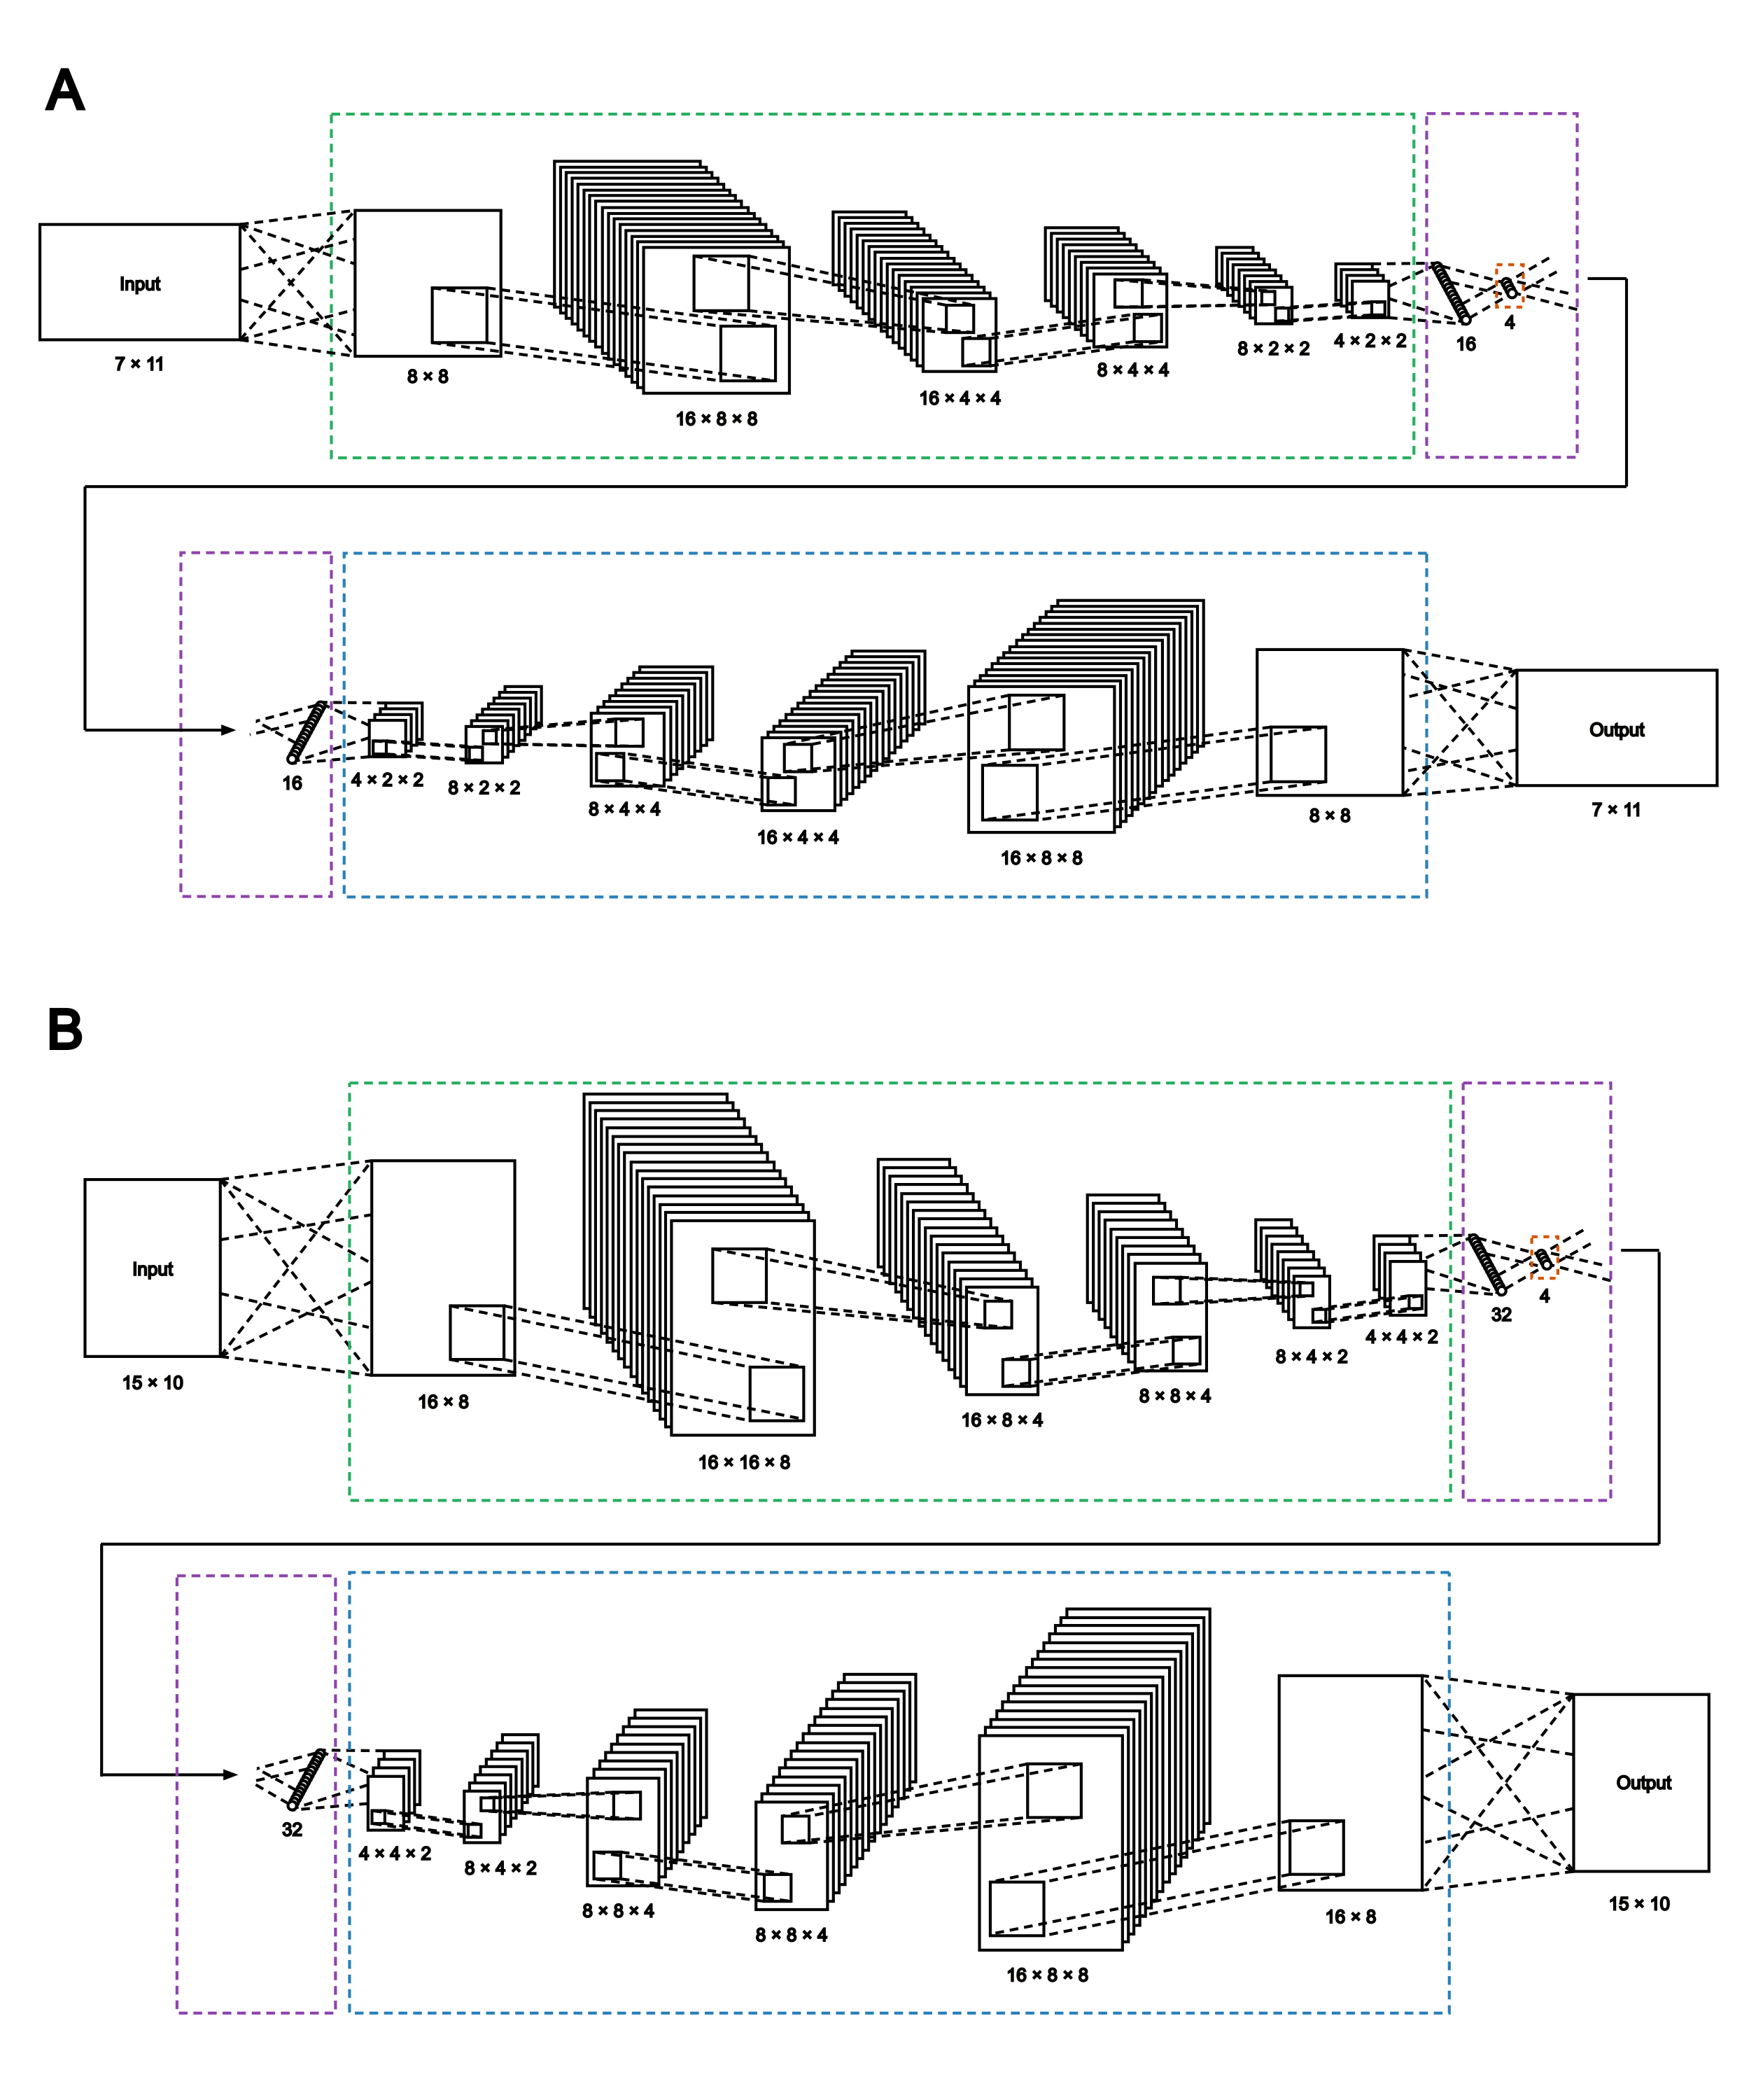
\includegraphics[width=0.9\columnwidth]{figures/CAE}
\caption{A table of various ARI values. \label{fig:ARI_table}%
}
\end{center}
\end{figure}

% SHOULD ACTUALLY BE A TABLE
\begin{figure}[H]
\begin{center}
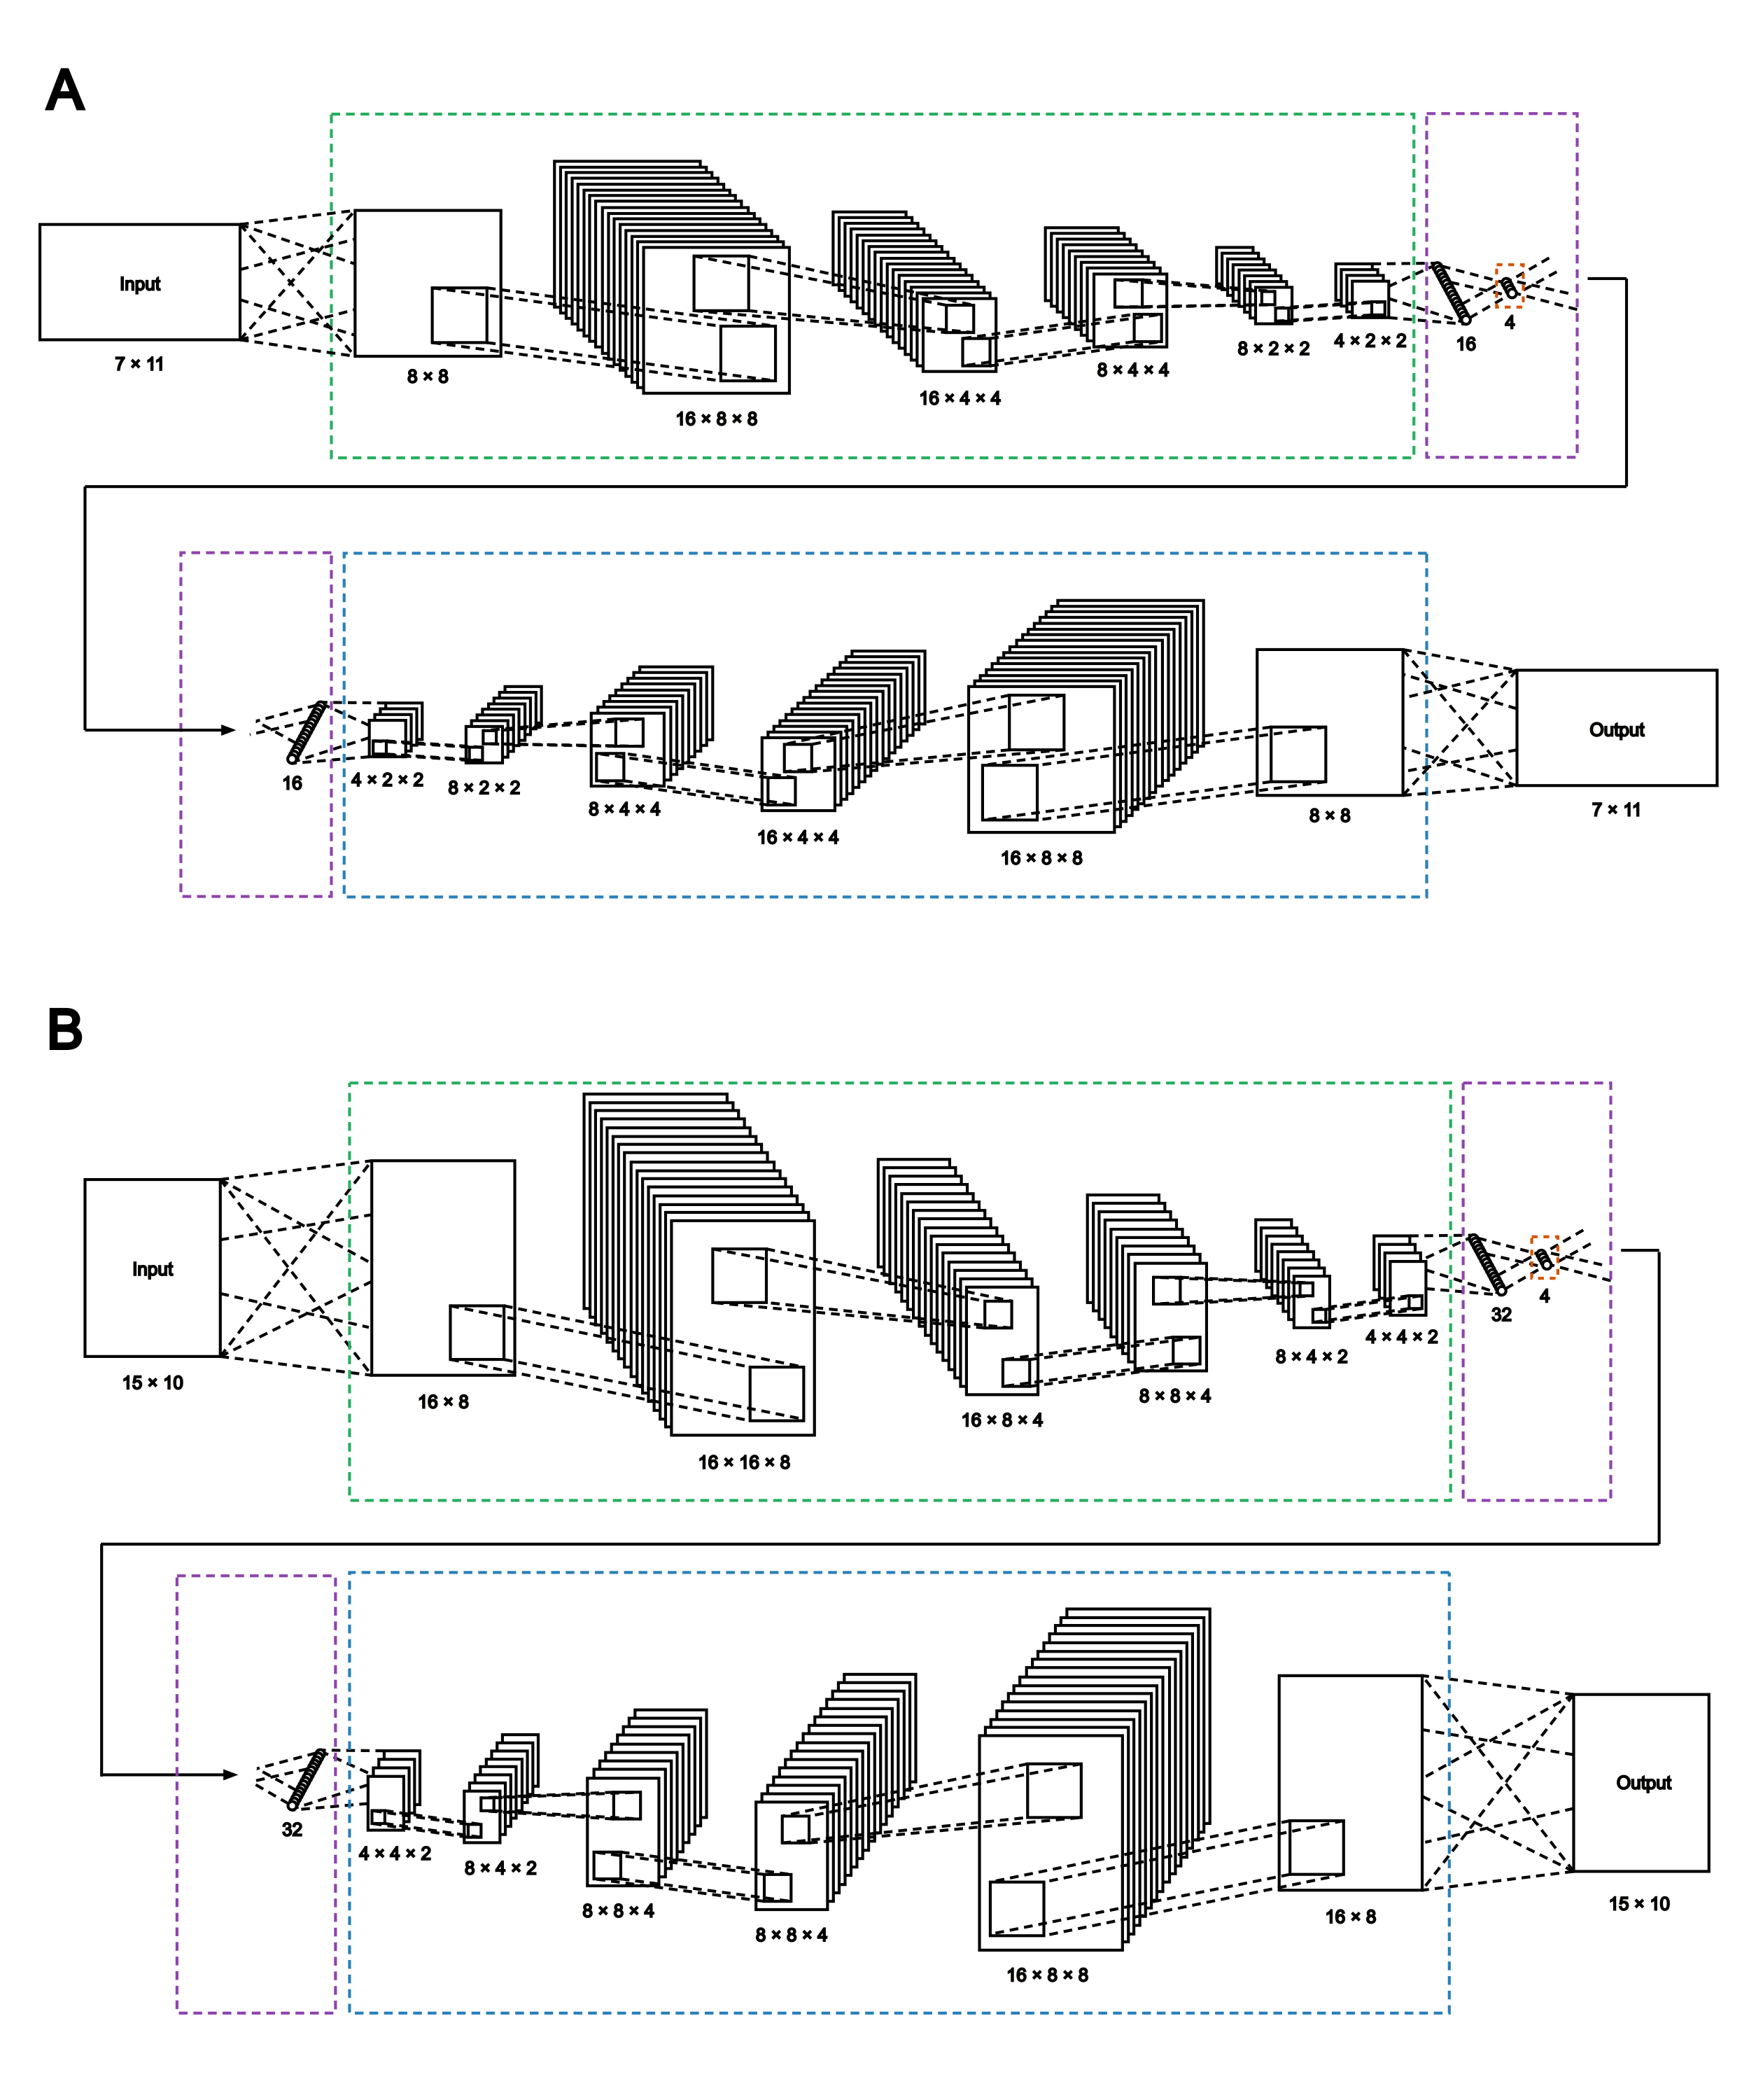
\includegraphics[width=0.9\columnwidth]{figures/CAE}
\caption{The homogeneity table between the two clusterings. \label{fig:homogeneity_table}%
}
\end{center}
\end{figure}

\begin{figure}[H]
\begin{center}
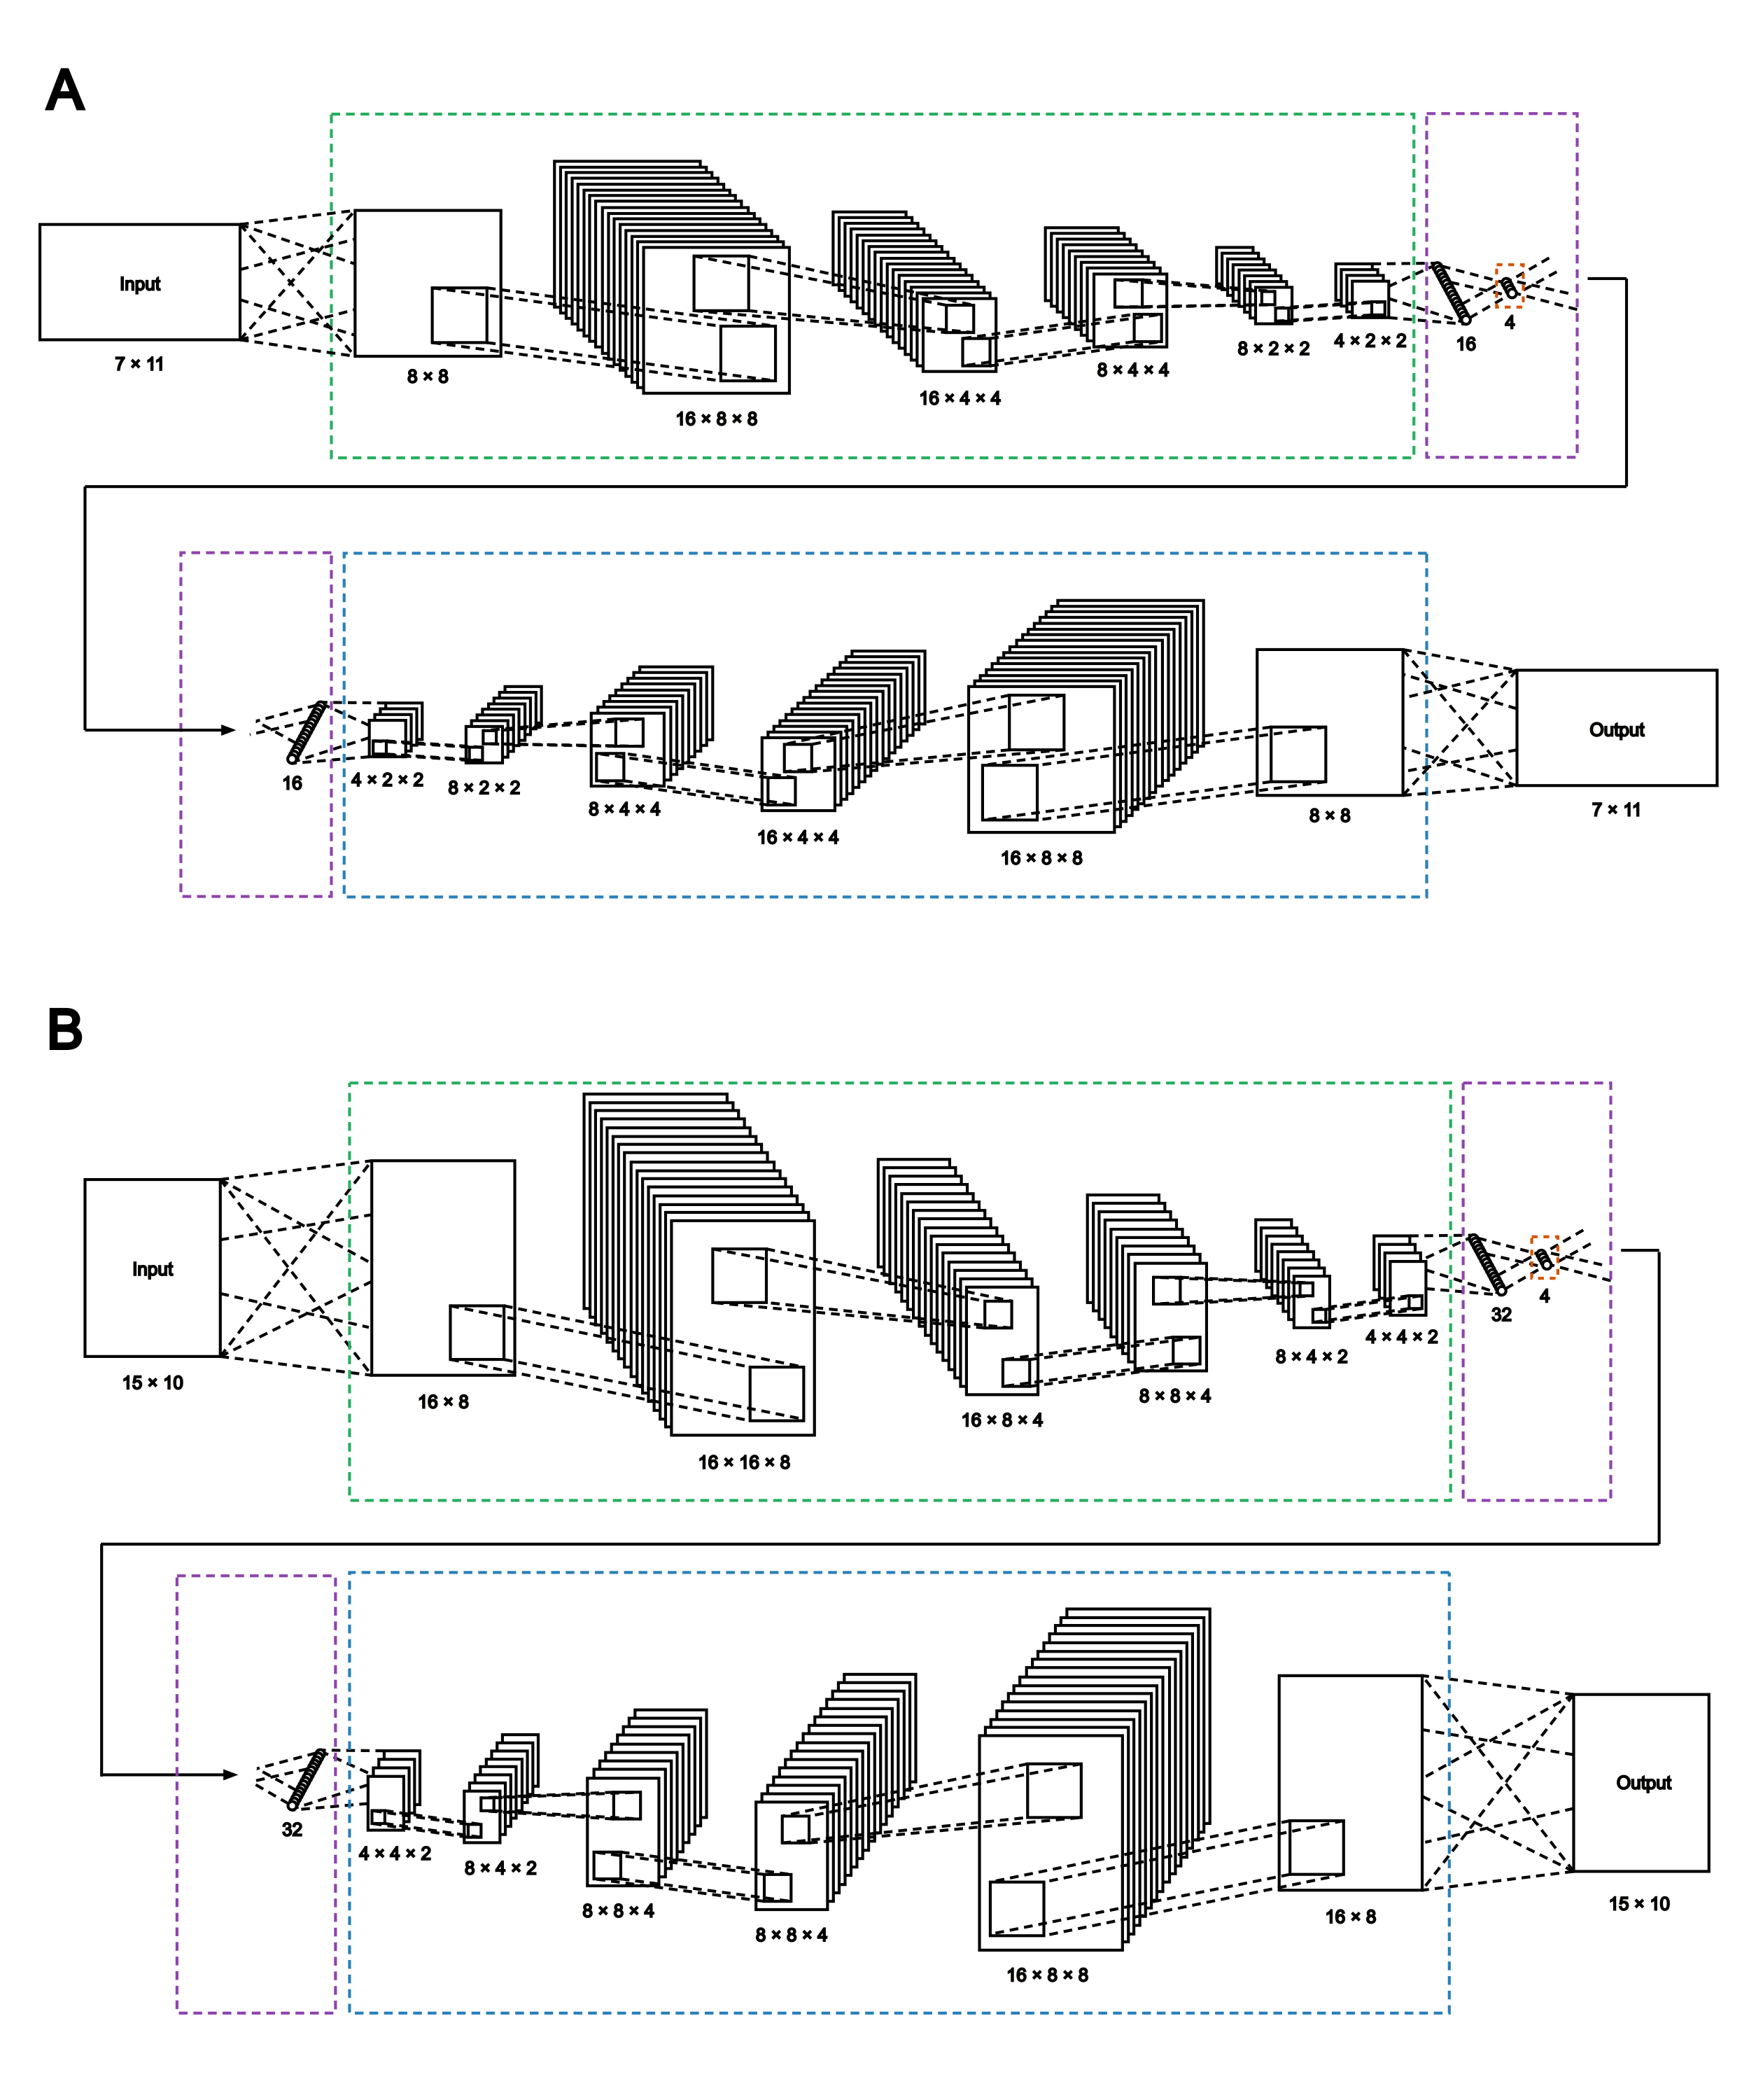
\includegraphics[width=0.9\columnwidth]{figures/CAE}
\caption{Cross-colored scatterplots reveal significant differences. \label{fig:cross_scatter}%
}
\end{center}
\end{figure}

\begin{figure}[H]
\begin{center}
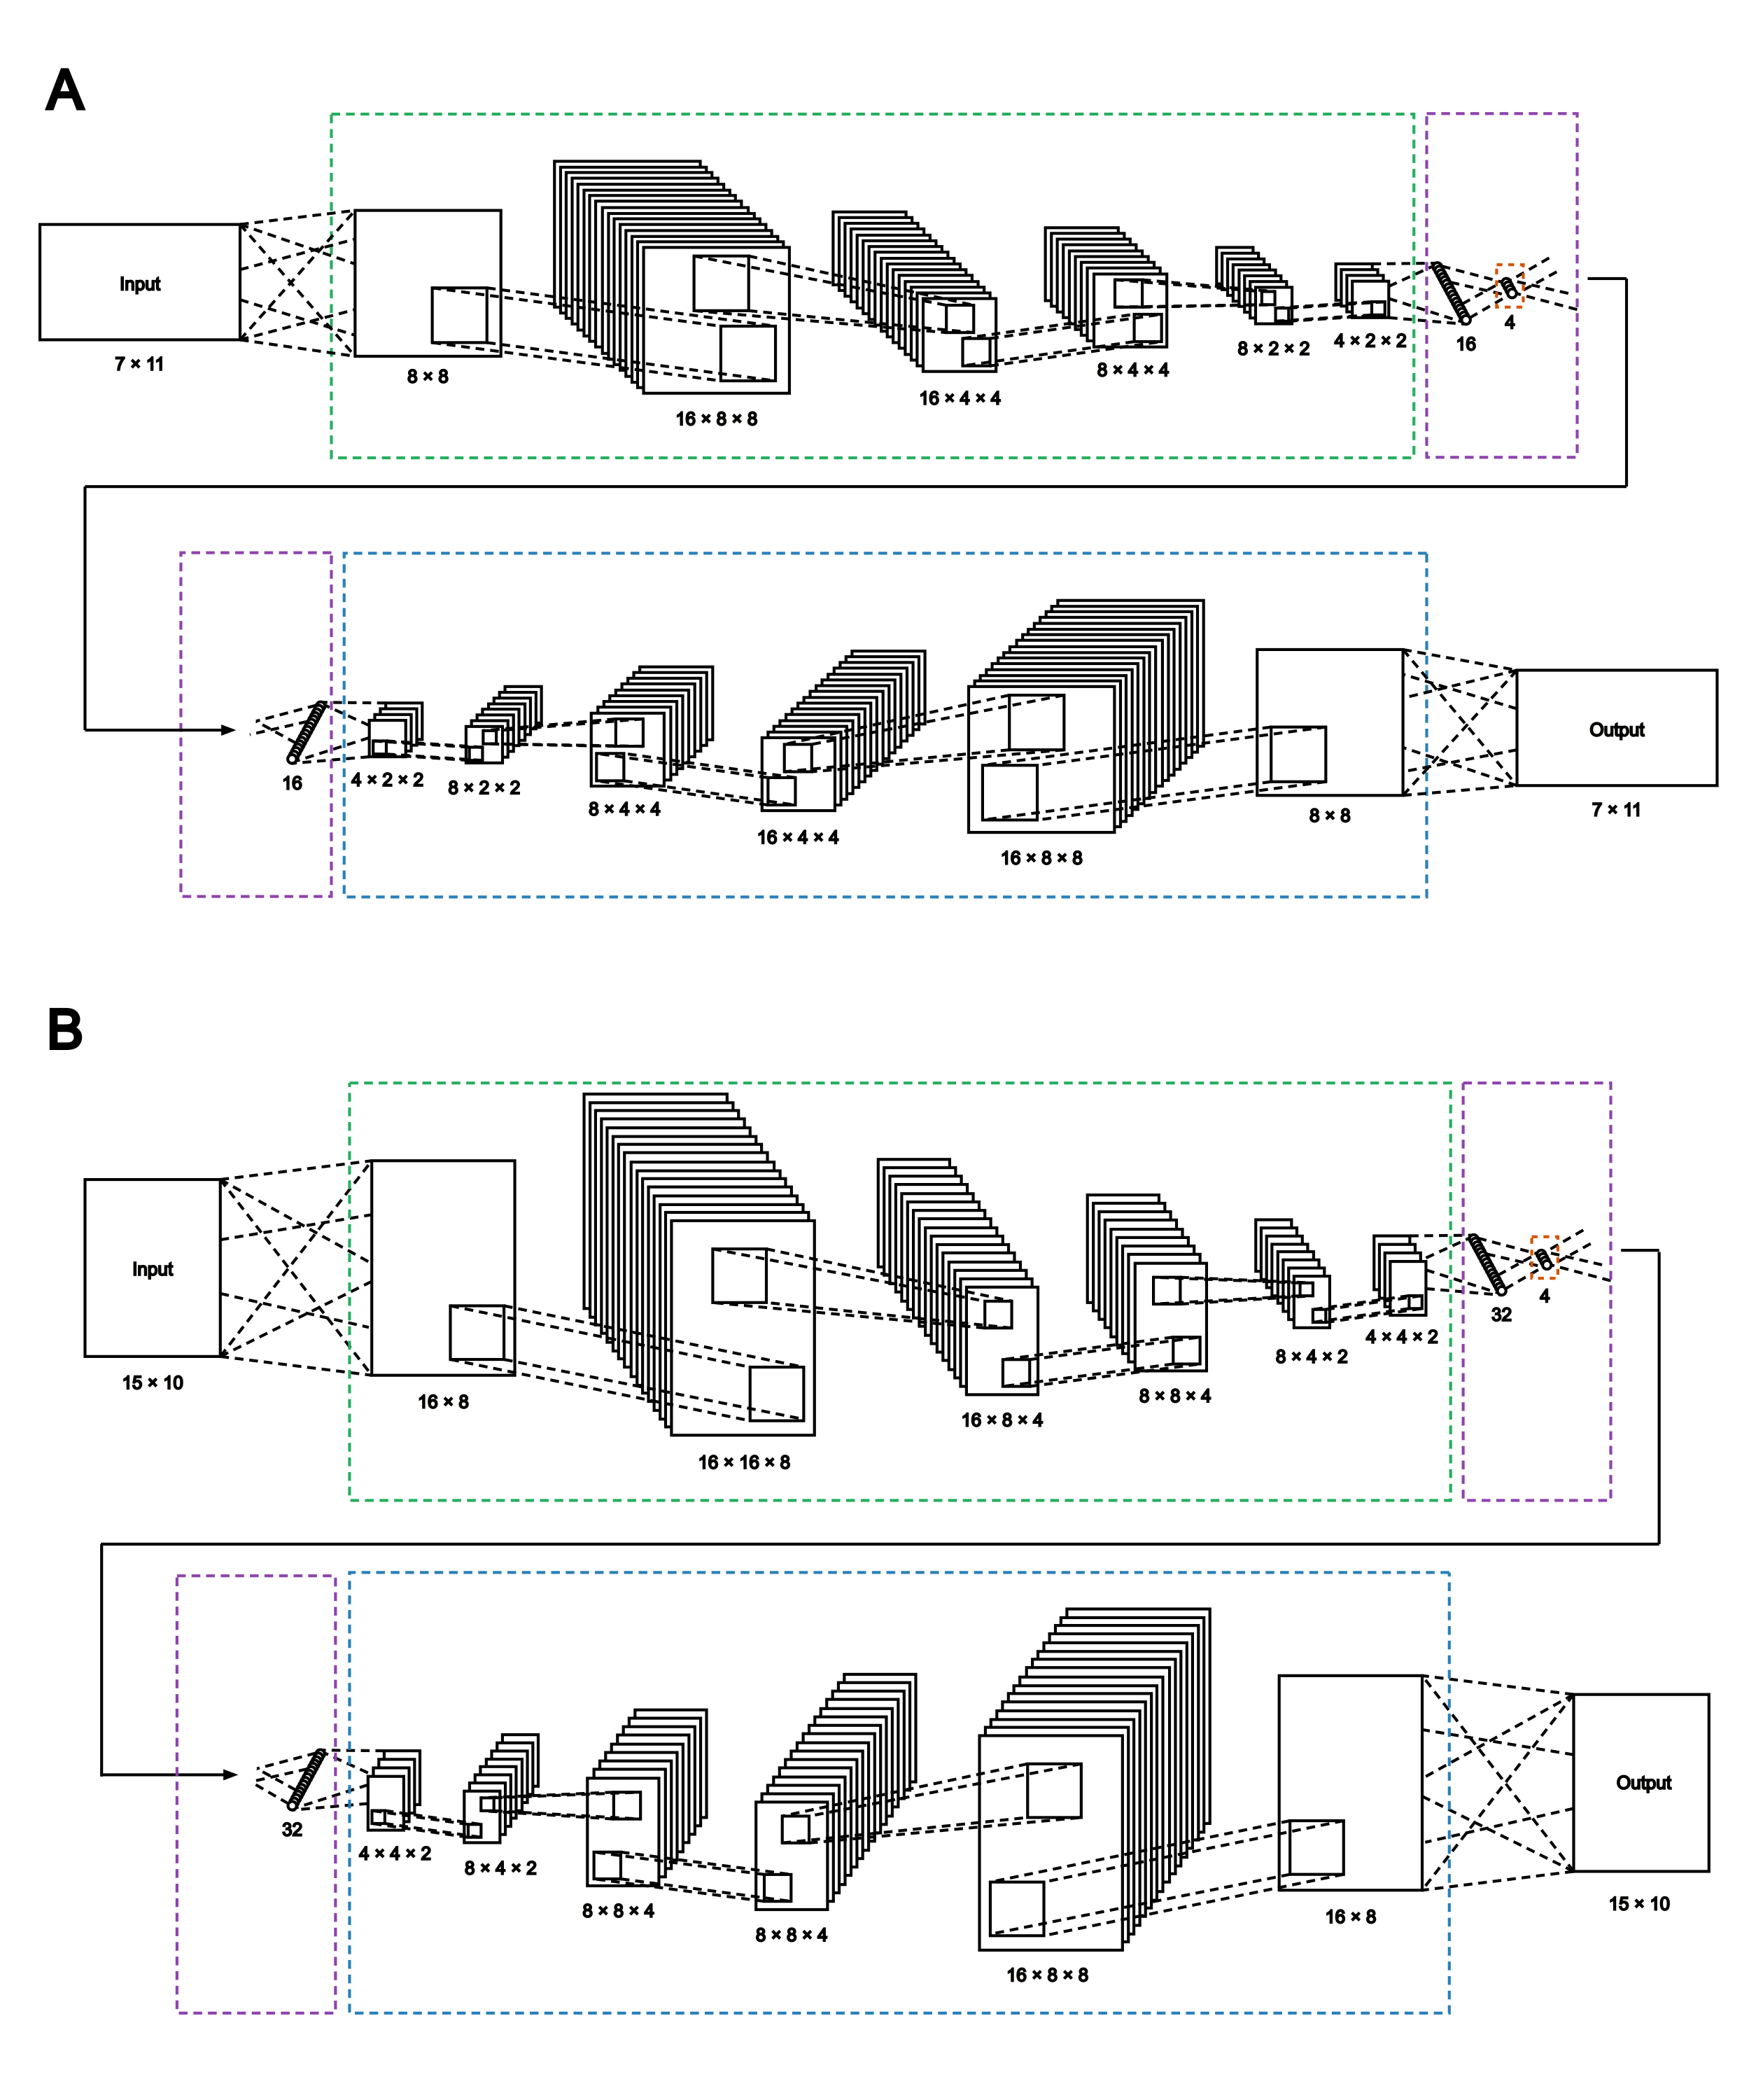
\includegraphics[width=0.9\columnwidth]{figures/CAE}
\caption{Cross- scatterplots can also be replaced with images. \label{fig:cross_image_scatter}%
}
\end{center}
\end{figure}

\section{Discussion}

\section{Conclusions}

\section{Limitations}

\section{Extensions}

\bibliographystyle{apa}
\bibliography{bibliography/biblio.bib%
}

\appendix

\section{Limitations and Assumptions}

This project was limited by the number of genes that were analyzed as well as the amount of expression data per gene. A central assumption, therefore, was that there was a sufficient number of genes and expression data for the results of the clustering to be determined by intrinsic differences and not variability. This assumption is supported by the relatively large number of genes (1,912) and expression data per gene (77 dimensions for mouse data, 150 for human data). Furthermore, the mouse and human donors used in this project were assumed to be representative of their respective populations. The regions of expression matrices were also assumed to be constant throughout development, which is supported by the high-accuracy computational methods used by the Allen Brain Atlas to quantize expression values.

\end{document}

